\documentclass[12pt,]{article}
%\usepackage{lmodern}  Melissa removed to deal with font rendering issue
\usepackage{amssymb,amsmath}
\usepackage{ifxetex,ifluatex}
\usepackage{fixltx2e} % provides \textsubscript

%Melissa removed the following section to deal with font rendering issue
%\ifnum 0\ifxetex 1\fi\ifluatex 1\fi=0 % if pdftex
%  \usepackage[T1]{fontenc}
%  \usepackage[utf8]{inputenc}
%%\else % if luatex or xelatex
%  \ifxetex
%    \usepackage{mathspec}
%  \else
%    \usepackage{fontspec}
%  \fi
%  \defaultfontfeatures{Ligatures=TeX,Scale=MatchLowercase}
%  \newcommand{\euro}{€}
%%%%%%\fi

% use upquote if available, for straight quotes in verbatim environments
\IfFileExists{upquote.sty}{\usepackage{upquote}}{}
% use microtype if available
\IfFileExists{microtype.sty}{%
\usepackage{microtype}
\UseMicrotypeSet[protrusion]{basicmath} % disable protrusion for tt fonts
}{}
\usepackage[margin=1in]{geometry}
\usepackage{hyperref}
\PassOptionsToPackage{usenames,dvipsnames}{color} % color is loaded by hyperref
\hypersetup{unicode=true,
            pdftitle={Status of Big Skate (Beringraja binoculata) Off the U.S. Pacific Coast in 2019},
            pdfborder={0 0 0},
            breaklinks=true}
\urlstyle{same}  % don't use monospace font for urls
\usepackage{graphicx,grffile}
\makeatletter
\def\maxwidth{\ifdim\Gin@nat@width>\linewidth\linewidth\else\Gin@nat@width\fi}
\def\maxheight{\ifdim\Gin@nat@height>\textheight\textheight\else\Gin@nat@height\fi}
\makeatother
% Scale images if necessary, so that they will not overflow the page
% margins by default, and it is still possible to overwrite the defaults
% using explicit options in \includegraphics[width, height, ...]{}
\setkeys{Gin}{width=\maxwidth,height=\maxheight,keepaspectratio}
\setlength{\parindent}{0pt}
\setlength{\parskip}{6pt plus 2pt minus 1pt}
\setlength{\emergencystretch}{3em}  % prevent overfull lines
\providecommand{\tightlist}{%
  \setlength{\itemsep}{0pt}\setlength{\parskip}{0pt}}
\setcounter{secnumdepth}{5}

%%% Use protect on footnotes to avoid problems with footnotes in titles
\let\rmarkdownfootnote\footnote%
\def\footnote{\protect\rmarkdownfootnote}

%%% Change title format to be more compact
\usepackage{titling}

% Create subtitle command for use in maketitle
\newcommand{\subtitle}[1]{
  \posttitle{
    \begin{center}\large#1\end{center}
    }
}

\setlength{\droptitle}{-2em}
  \title{Status of Big Skate (\emph{Beringraja binoculata}) Off the U.S. Pacific
Coast in 2019}
  \pretitle{\vspace{\droptitle}\centering\huge}
  \posttitle{\par}
  \author{}
  \preauthor{}\postauthor{}
  \date{}
  \predate{}\postdate{}


% This file contains all of the LaTeX packages you may need to compile the document
% Documentation for each package can be found onlines
\usepackage{tabularx}                                             % table environment providing flexibility
\usepackage{caption}                                              % for creating captions  
\usepackage{longtable}                                            % allows tables to span multiple pages
\usepackage{rotating}                                             % allows for sideways tables
\usepackage{float}                                                % floating environments; may not need in rmarkdown
\usepackage{placeins}                                             % keeps floats from moving
\usepackage{indentfirst}                                          % indents first paragraph of a section
\usepackage{mdwtab}                                               % continued float multi-page figure
\usepackage{enumerate}                                            % create lists
\usepackage{hyperref}                                             % highlight cross references
\hypersetup{colorlinks=true, urlcolor=blue, linktoc=page, linkcolor=blue, citecolor=blue} %define referencing colors
%\usepackage{makebox}                                             % make boxes around text
\usepackage[usenames,dvipsnames]{xcolor}                          % color name options
%\usepackage[space]{grffile}                                      % spaces in file name path
\usepackage{soul}                                                 % highlight text
\usepackage{enumitem}                                             % numbered lists
\usepackage{lineno}                                               % Line numbers; comment out for final
\usepackage{upquote}                                              % produce grave accent in latex
\usepackage{verbatim}                                             % produces verbatim results
\usepackage{fancyvrb}                                             % verbatim in a box
%\usepackage{draftwatermark}                                      % places Draft watermark in background; comment out for final
\usepackage{textcomp}                                             % fixes error with packages interfering
\usepackage{lscape}                                               % rotate pages - to allow for landscape longtables
%\pdfinterwordspaceon                                             % fix loss of inter word spacing
\usepackage{cmap}                                                 % fix mapping characters to unicode
\RequirePackage[linewidth = 1]{pdfcomment}                        % pdf comments
\RequirePackage[l2tabu, orthodox]{nag}                            % checks packages related to the accessibility?
\usepackage[inline]{showlabels}                                   % show table and figure labels; comment out for final
%\RequirePackage[tagged]{accessibilityMeta}
\usepackage{pdflscape}                                            % For horizontal format
\usepackage{booktabs}                                             % For multi-header tables

\linenumbers                                                      % specify use of line numbers


\definecolor{light-gray}{gray}{.85}                               % define light-gray as a color
%\usepackage[tagged]{accessibility-meta}

 
%\showlabels[\color{mred}]{label}

% Redefines (sub)paragraphs to behave more like sections
\ifx\paragraph\undefined\else
\let\oldparagraph\paragraph
\renewcommand{\paragraph}[1]{\oldparagraph{#1}\mbox{}}
\fi
\ifx\subparagraph\undefined\else
\let\oldsubparagraph\subparagraph
\renewcommand{\subparagraph}[1]{\oldsubparagraph{#1}\mbox{}}
\fi

\begin{document}
\maketitle


\begin{center}
\thispagestyle{empty}

\vspace{.7cm}

% 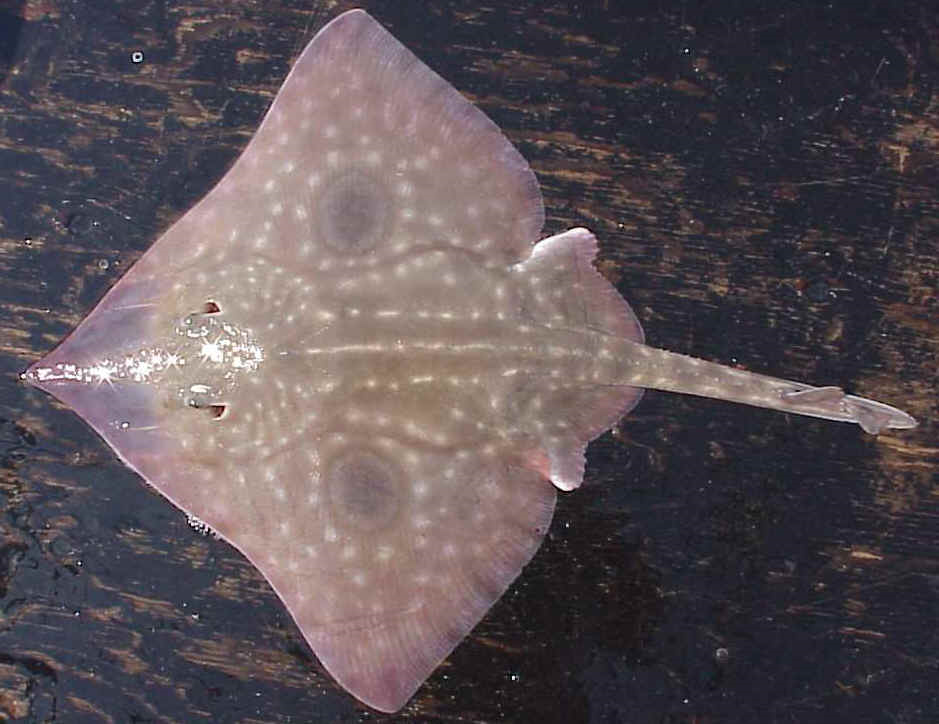
\includegraphics{cover_photo}~\\[1cm]
\pdftooltip{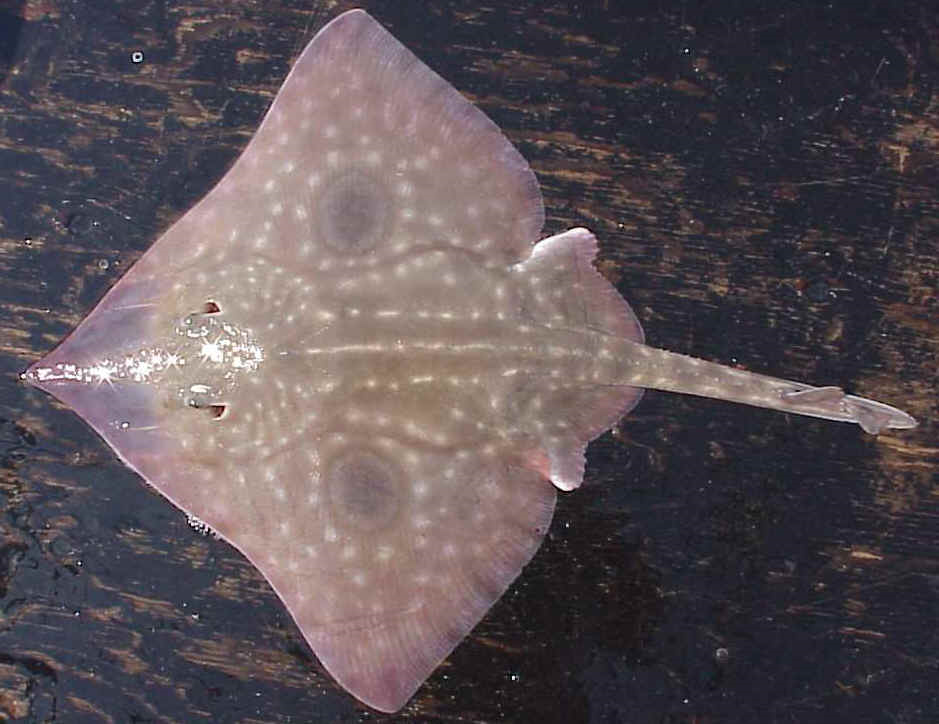
\includegraphics{cover_photo}}{This is a fish.}

\vspace{.5cm}

Ian G. Taylor\textsuperscript{1}\\
Vladlena Gertseva\textsuperscript{1}\\
Joseph Bizzarro\textsuperscript{2}\\
Andi Stephens\textsuperscript{3}\\

\vspace{.7cm}

\small

\textsuperscript{1}Northwest Fisheries Science Center, U.S. Department of Commerce, National Oceanic and Atmospheric Administration, National Marine Fisheries Service, 2725 Montlake Boulevard East, Seattle, Washington 98112\\

\vspace{.3cm}

\textsuperscript{2}Southwest Fisheries Science Center, U.S. Department of Commerce, National Oceanic and Atmospheric Administration, National Marine Fisheries Service, 110 Shaffer Road, Santa Cruz, California 95060\\

\vspace{.3cm}

\textsuperscript{3}Northwest Fisheries Science Center, U.S. Department of Commerce, National Oceanic and Atmospheric Administration, National Marine Fisheries Service, 2032 S.E. OSU Drive Newport, Oregon 97365


\vspace{.5cm}

\vfill
DRAFT SAFE\\
Disclaimer: This information is distributed solely for the purpose of pre-dissemination
peer review under applicable information quality guidelines. It has not been formally
disseminated by NOAA Fisheries. It does not represent and should not be construed to
represent any agency determination or policy. 

\vspace{.3cm}
%Bottom of the page
%{\large \today}


\newpage{\thispagestyle{empty}}

\vspace*{\fill}
\begin{flushleft}
This report may be cited as:

Taylor, I.G., Gertseva, V., Bizzarro, J., and Stephens, A. Status of Big Skate (\emph{Beringraja binoculata}) Off the U.S. West Coast, 2019. Pacific Fishery Management Council, Portland, OR. Available from http://www.pcouncil.org/groundfish/stock-assessments/
\end{flushleft}

\maketitle

\pagenumbering{roman}
\setcounter{page}{1}
\end{center}

{
\setcounter{tocdepth}{4}
\tableofcontents
}
\setlength{\parskip}{5mm plus1mm minus1mm}
\pagebreak

\pagenumbering{arabic}

\renewcommand{\thefigure}{\alph{figure}}
\renewcommand{\thetable}{\alph{table}}

\hypertarget{executive-summary}{%
\section*{Executive Summary}\label{executive-summary}}
\addcontentsline{toc}{section}{Executive Summary}

\hypertarget{stock}{%
\subsection*{Stock}\label{stock}}
\addcontentsline{toc}{subsection}{Stock}

This assessment reports the status of the Big Skate
(\emph{Beringraja binoculata}) resource in U.S. waters off the West
Coast using data through 2018.

\hypertarget{catches}{%
\subsection*{Catches}\label{catches}}
\addcontentsline{toc}{subsection}{Catches}

Landings and estimated discards of Big Skate were reconstructed for this
assessment from historical records of other species and from species
composition data collected in the recent fishery. These reflect the
fishery from 1916-1994. The current fishery started in 1995. For records
from 1995-2017, Big Skate landings were estimated from
species-composition samples and the landings of ``Unspecified Skates''.
Beginning in 2017, Big Skate have been recorded in species-specific
landings.

(Table \ref{tab:Exec_catch}).

(Figures \ref{fig:Exec_catch1}-\ref{fig:Exec_catch2})\\
(Figure \ref{fig:r4ss_catches})

In the current fishery (since 1995), annual total landings of Big Skate
have ranged between 135-528 mt, with landings in 2018 totaling 173 mt.

\FloatBarrier

\FloatBarrier

\begin{figure}
\centering
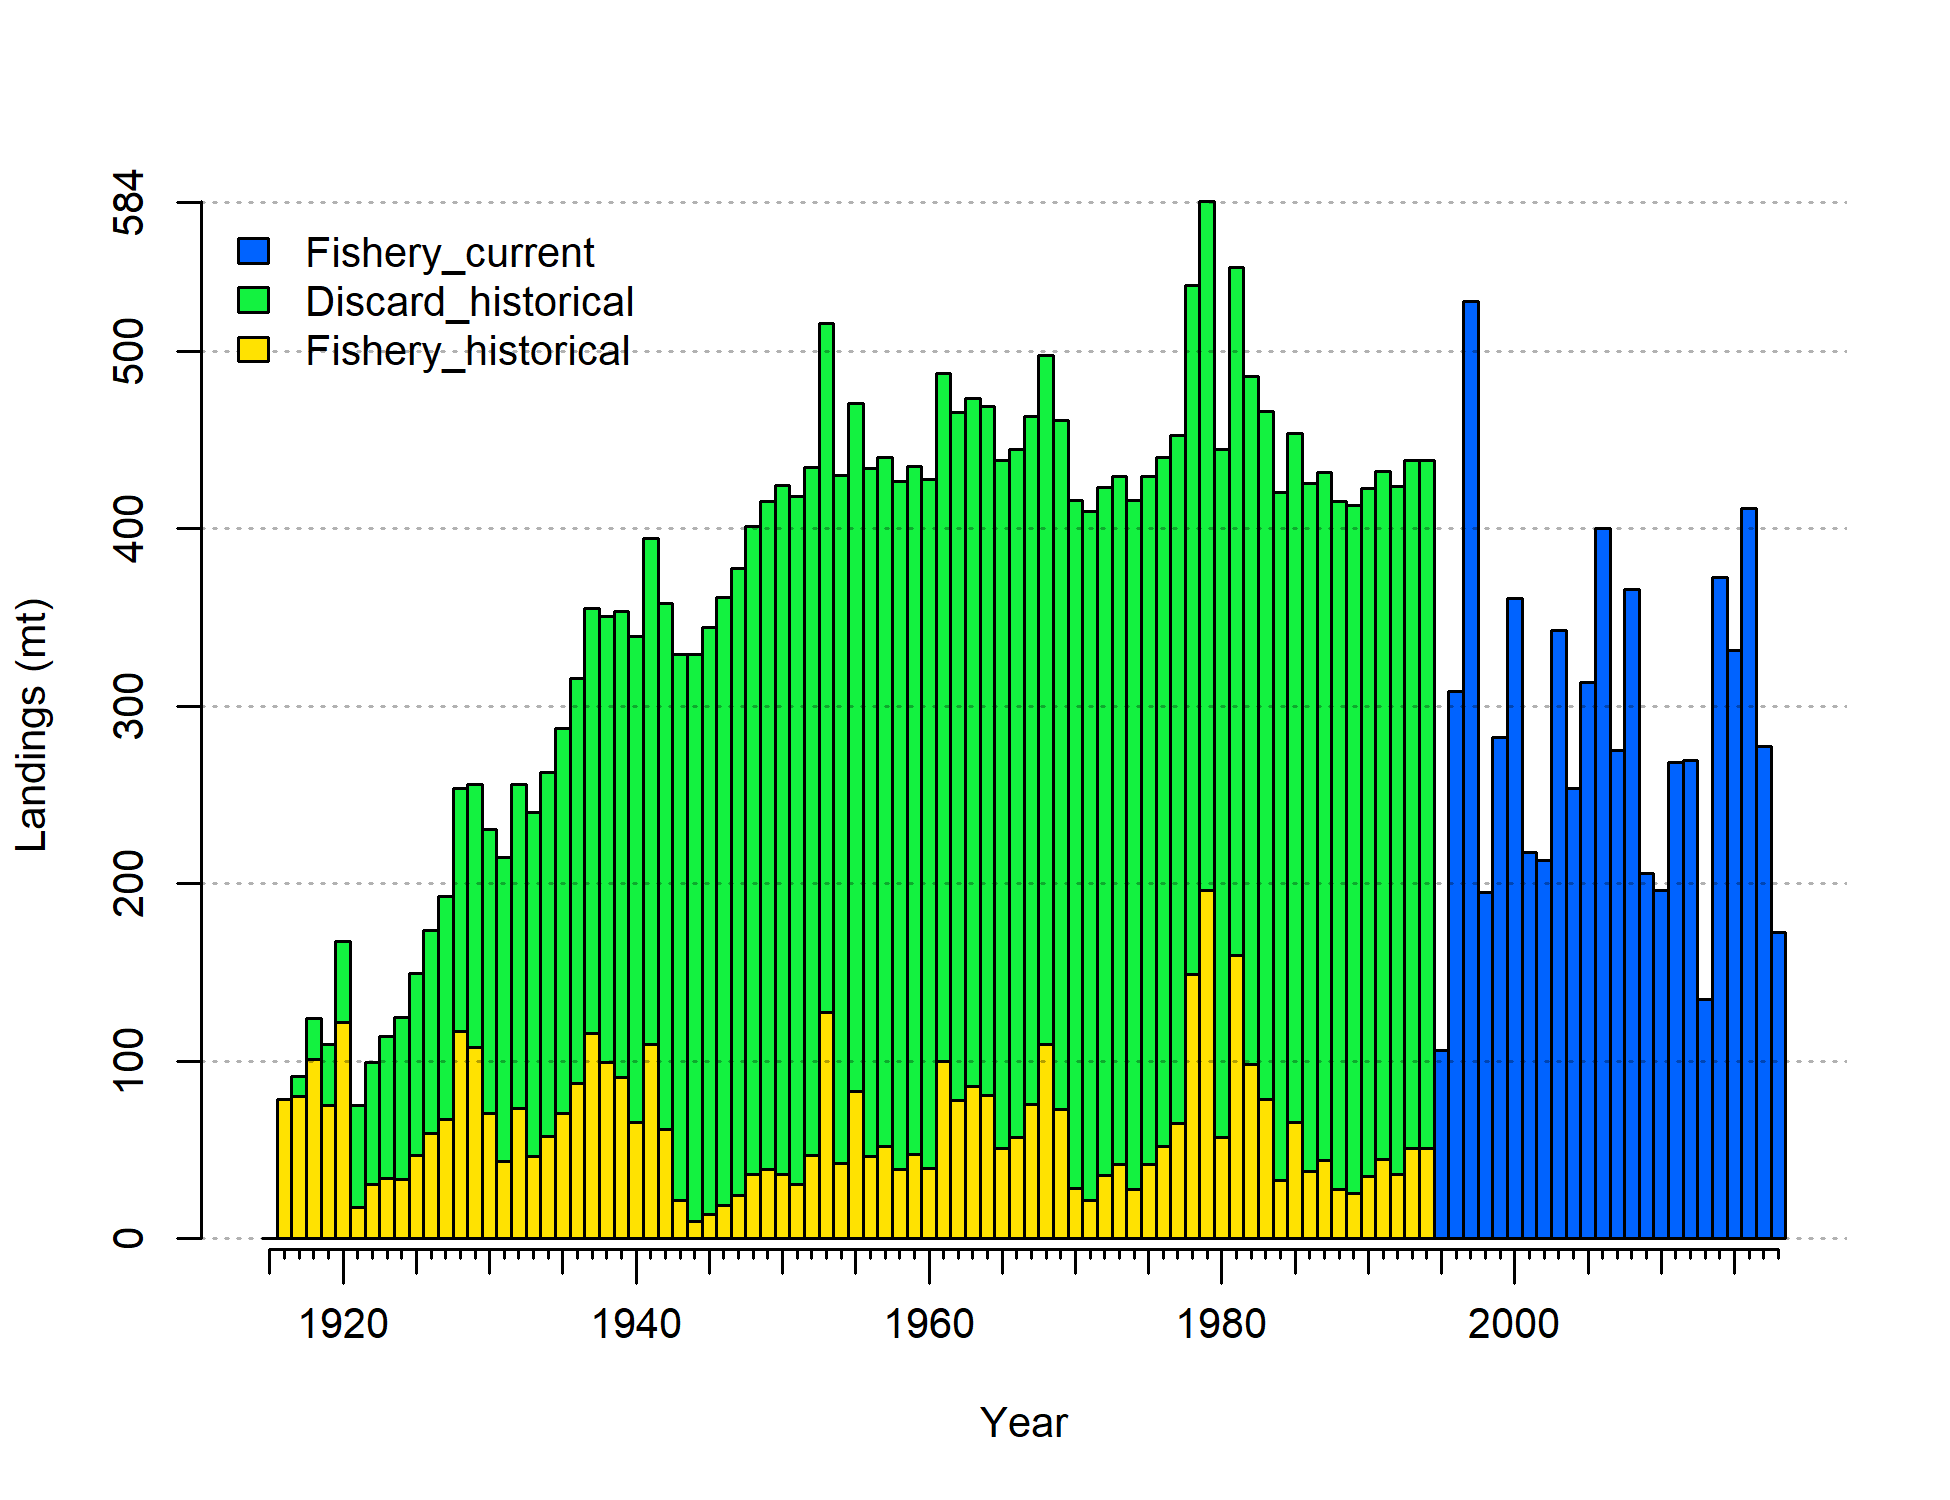
\includegraphics{r4ss/plots_mod1/catch2 landings stacked.png}
\caption{Catch history of Big Skate in the model.
\label{fig:r4ss_catches}}
\end{figure}

\begin{table}[ht]
\centering
\caption{Recent Big Skate landings (mt)} 
\label{tab:Exec_catch}
\begin{tabular}{l>{\centering}p{.6in}}
  \hline
Year & Landings \\ 
  \hline
2008 & 366.00 \\ 
  2009 & 205.70 \\ 
  2010 & 196.20 \\ 
  2011 & 268.40 \\ 
  2012 & 269.60 \\ 
  2013 & 135.00 \\ 
  2014 & 372.40 \\ 
  2015 & 331.50 \\ 
  2016 & 411.50 \\ 
  2017 & 277.60 \\ 
  2018 & 172.60 \\ 
   \hline
\end{tabular}
\end{table}

\FloatBarrier

\newpage

\hypertarget{data-and-assessment}{%
\subsection*{Data and Assessment}\label{data-and-assessment}}
\addcontentsline{toc}{subsection}{Data and Assessment}

This the first full assessment for Big Skate, which was last assessed as
part of the ``Other Species'' complex. This assessment uses the newest
version of Stock Synthesis (3.30.13). The model begins in 1916, and
assumes the stock was at an unfished equilibrium that year.

(Figure \ref{fig:assess_region_map}).

\begin{figure}
\centering
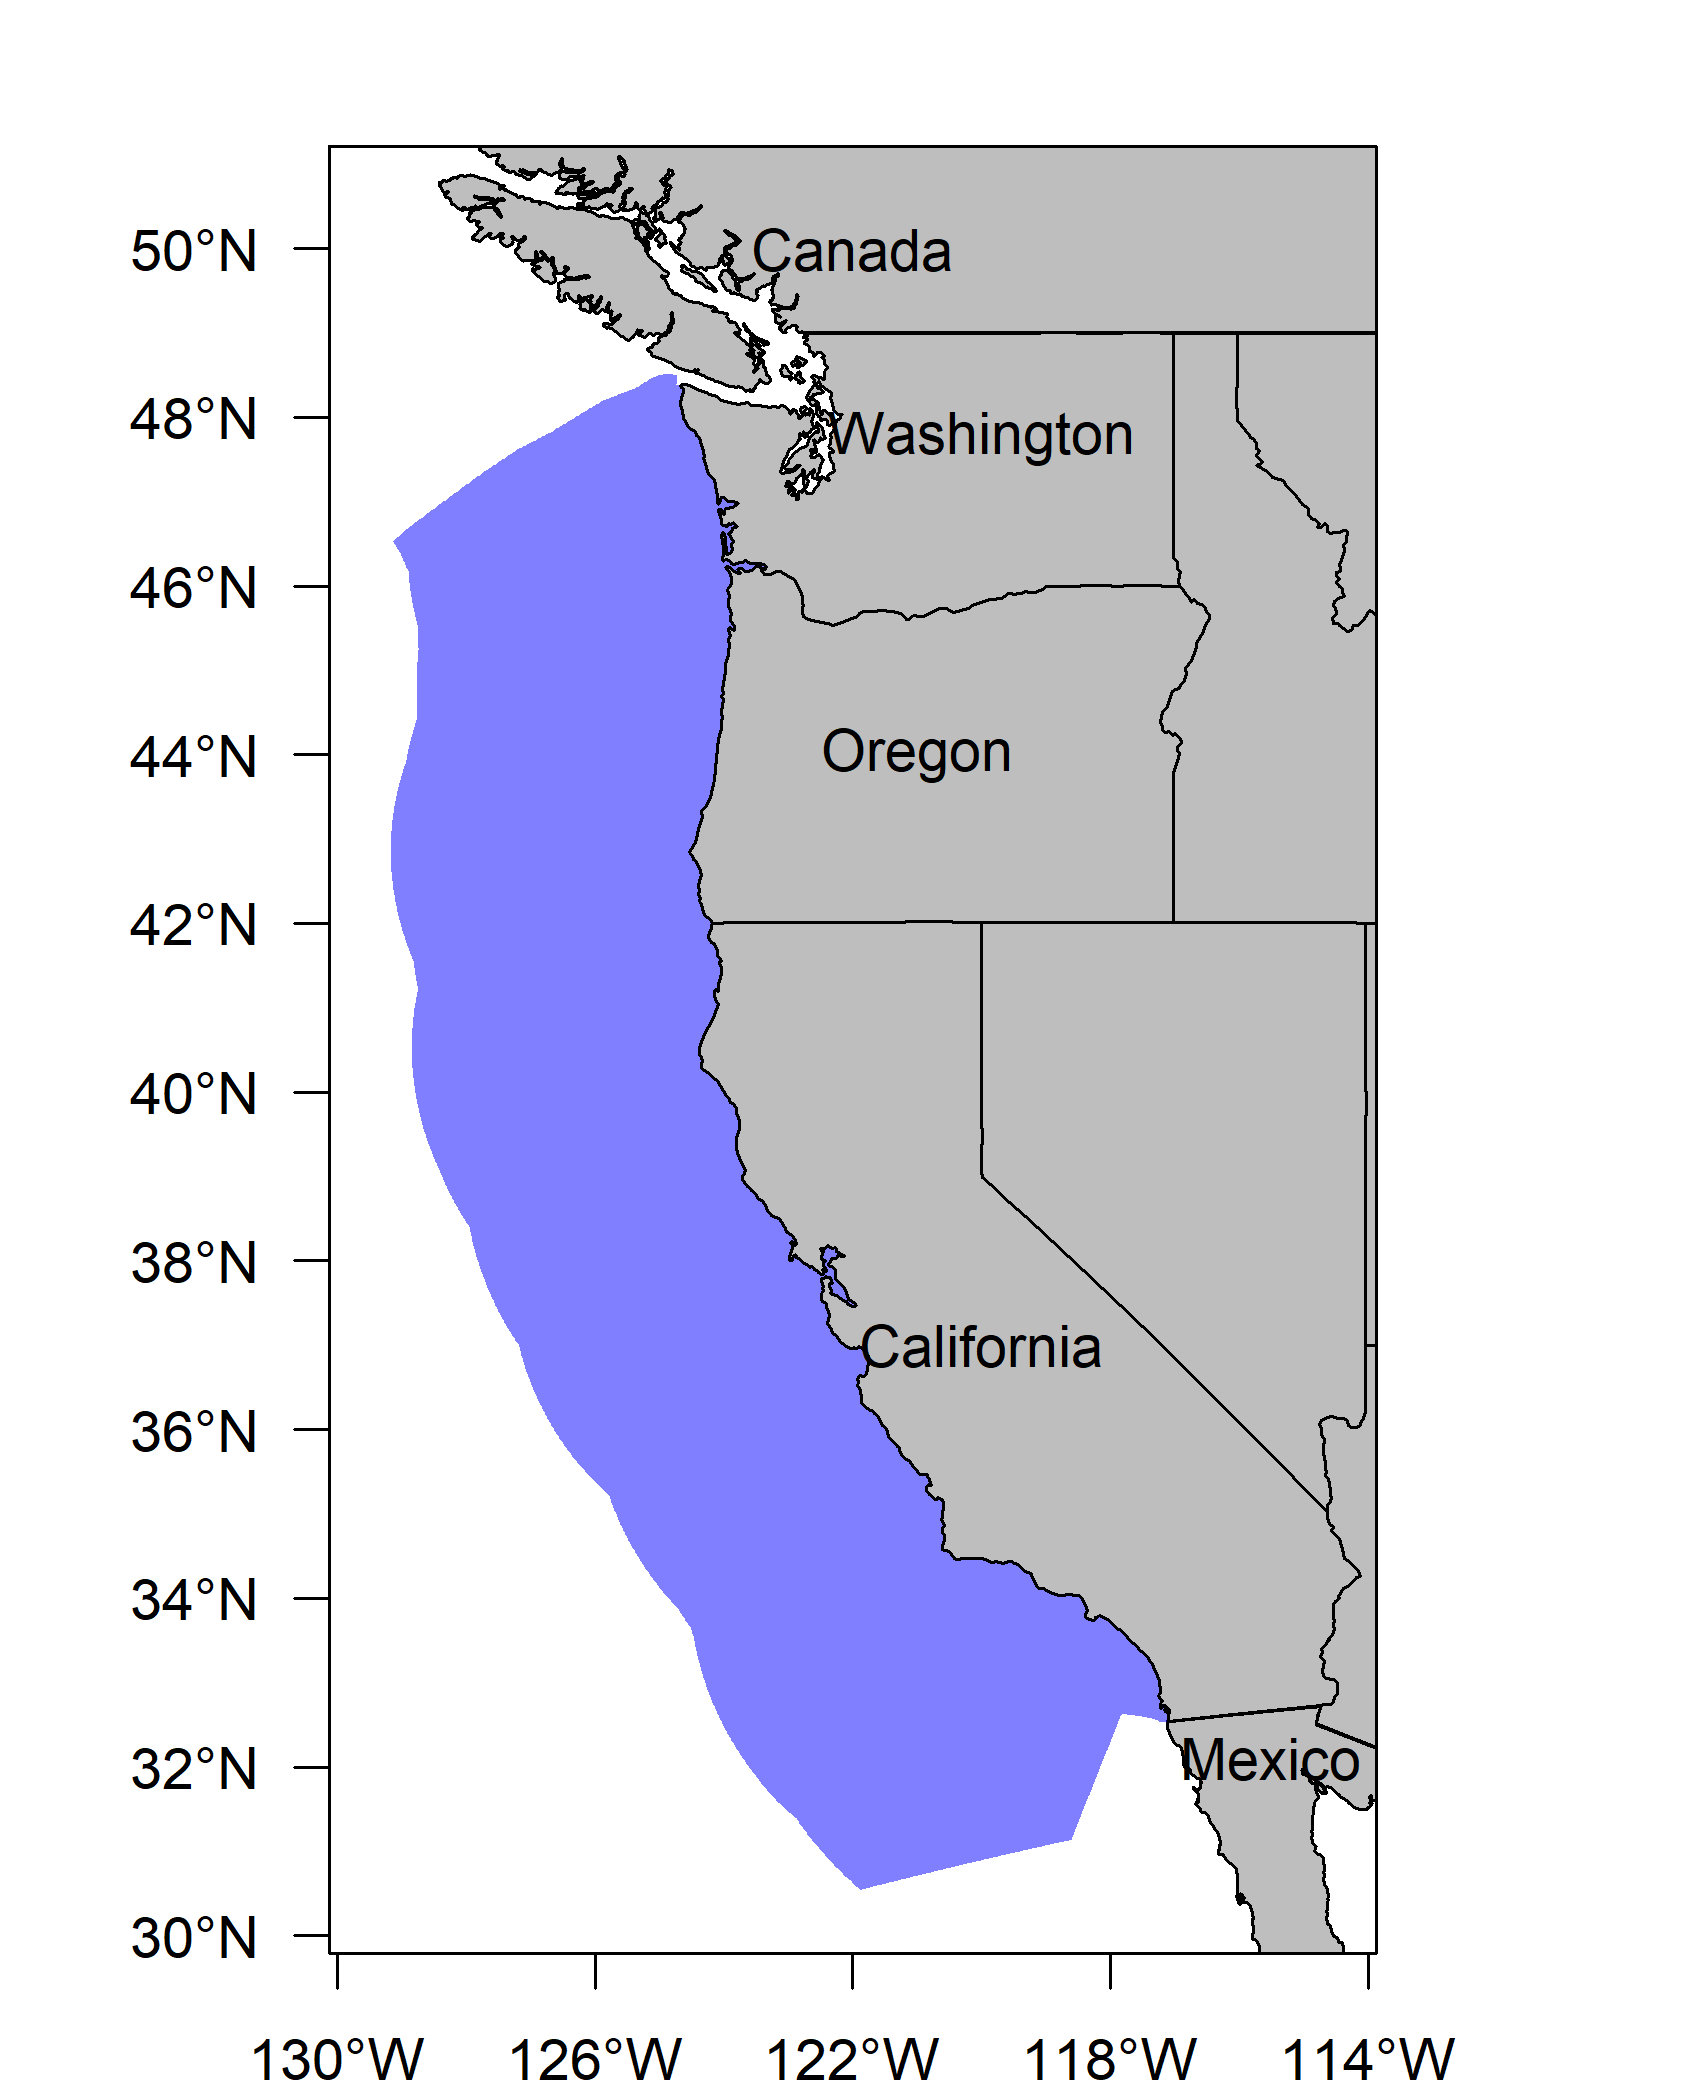
\includegraphics{Figures/assess_region_map.png}
\caption{This is NOT the map depicting the distribution of Big Skate out
to 600 ft. The stock assessment is bounded at Pt. Conception in the
South to the U.S./Canada border in the north.
\label{fig:assess_region_map}}
\end{figure}

\FloatBarrier

\hypertarget{stock-biomass}{%
\subsection*{Stock Biomass}\label{stock-biomass}}
\addcontentsline{toc}{subsection}{Stock Biomass}

(Figure \ref{fig:Spawnbio_all} and Table
\ref{tab:SpawningDeplete_mod1}).

The 2018 estimated spawning biomass relative to unfished equilibrium
spawning biomass is above the target of 40\% of unfished spawning
biomass at 72.5\% (95\% asymptotic interval: \(\pm\) 55.2\%-89.7\%)
(Figure \ref{fig:RelDeplete_all}). Approximate confidence intervals
based on the asymptotic variance estimates show that the uncertainty in
the estimated spawning biomass is high.

\FloatBarrier

\begin{table}[ht]
\centering
\caption{Recent trend in beginning of the 
                                      year spawning output and depletion for
                                      the model for Big Skate.} 
\label{tab:SpawningDeplete_mod1}
\begin{tabular}{l>{\centering}p{1.3in}>{\centering}p{1.2in}>{\centering}p{1in}>{\centering}p{1.2in}}
  \hline
Year & Spawning Output (million eggs) & \~{} 95\% confidence interval & Estimated depletion & \~{} 95\% confidence interval \\ 
  \hline
2010 & 1059.250 & (425.78-1692.72) & 0.694 & (0.552-0.837) \\ 
  2011 & 1068.670 & (434.08-1703.26) & 0.700 & (0.56-0.841) \\ 
  2012 & 1073.990 & (438.95-1709.03) & 0.704 & (0.564-0.843) \\ 
  2013 & 1079.980 & (444.55-1715.41) & 0.708 & (0.57-0.846) \\ 
  2014 & 1094.970 & (458.25-1731.69) & 0.718 & (0.583-0.852) \\ 
  2015 & 1095.100 & (458.91-1731.29) & 0.718 & (0.583-0.852) \\ 
  2016 & 1097.700 & (461.69-1733.71) & 0.719 & (0.586-0.853) \\ 
  2017 & 1093.720 & (458.52-1728.92) & 0.717 & (0.583-0.851) \\ 
  2018 & 1097.080 & (461.78-1732.38) & 0.719 & (0.586-0.852) \\ 
  2019 & 1106.070 & (504.33-1707.81) & 0.725 & (0.552-0.897) \\ 
   \hline
\end{tabular}
\end{table}

\FloatBarrier

\begin{figure}
\centering
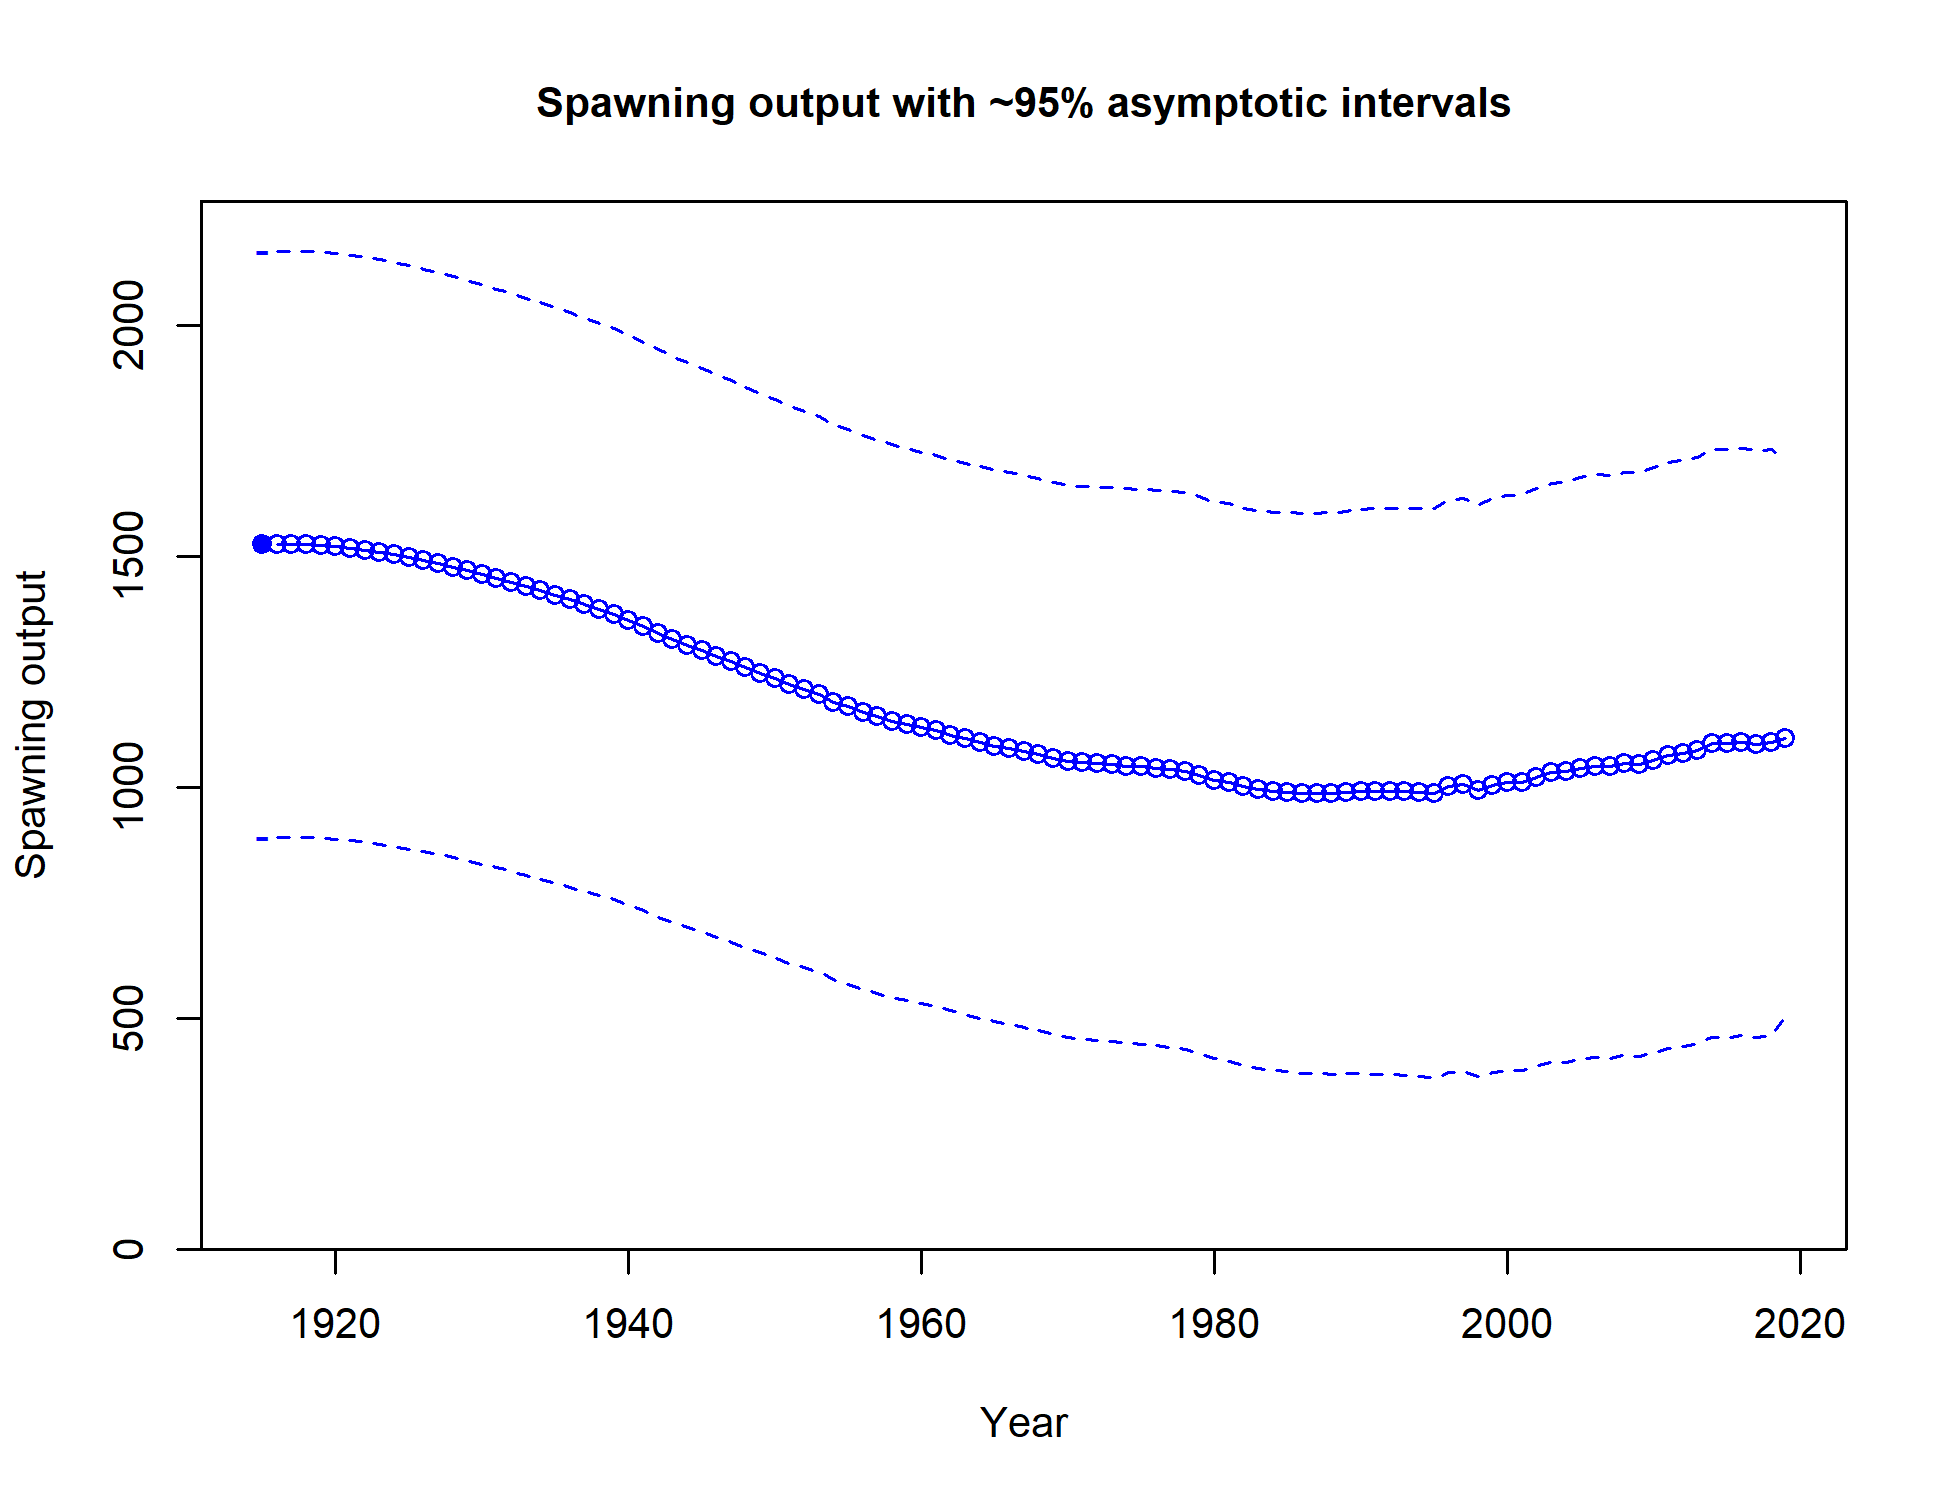
\includegraphics{r4ss/plots_mod1/ts7_Spawning_output_with_95_asymptotic_intervals_intervals.png}
\caption{Time series of spawning biomass trajectory (circles and line:
median; light broken lines: 95\% credibility intervals) for the base
case assessment model. \label{fig:Spawnbio_all}}
\end{figure}

\begin{figure}
\centering
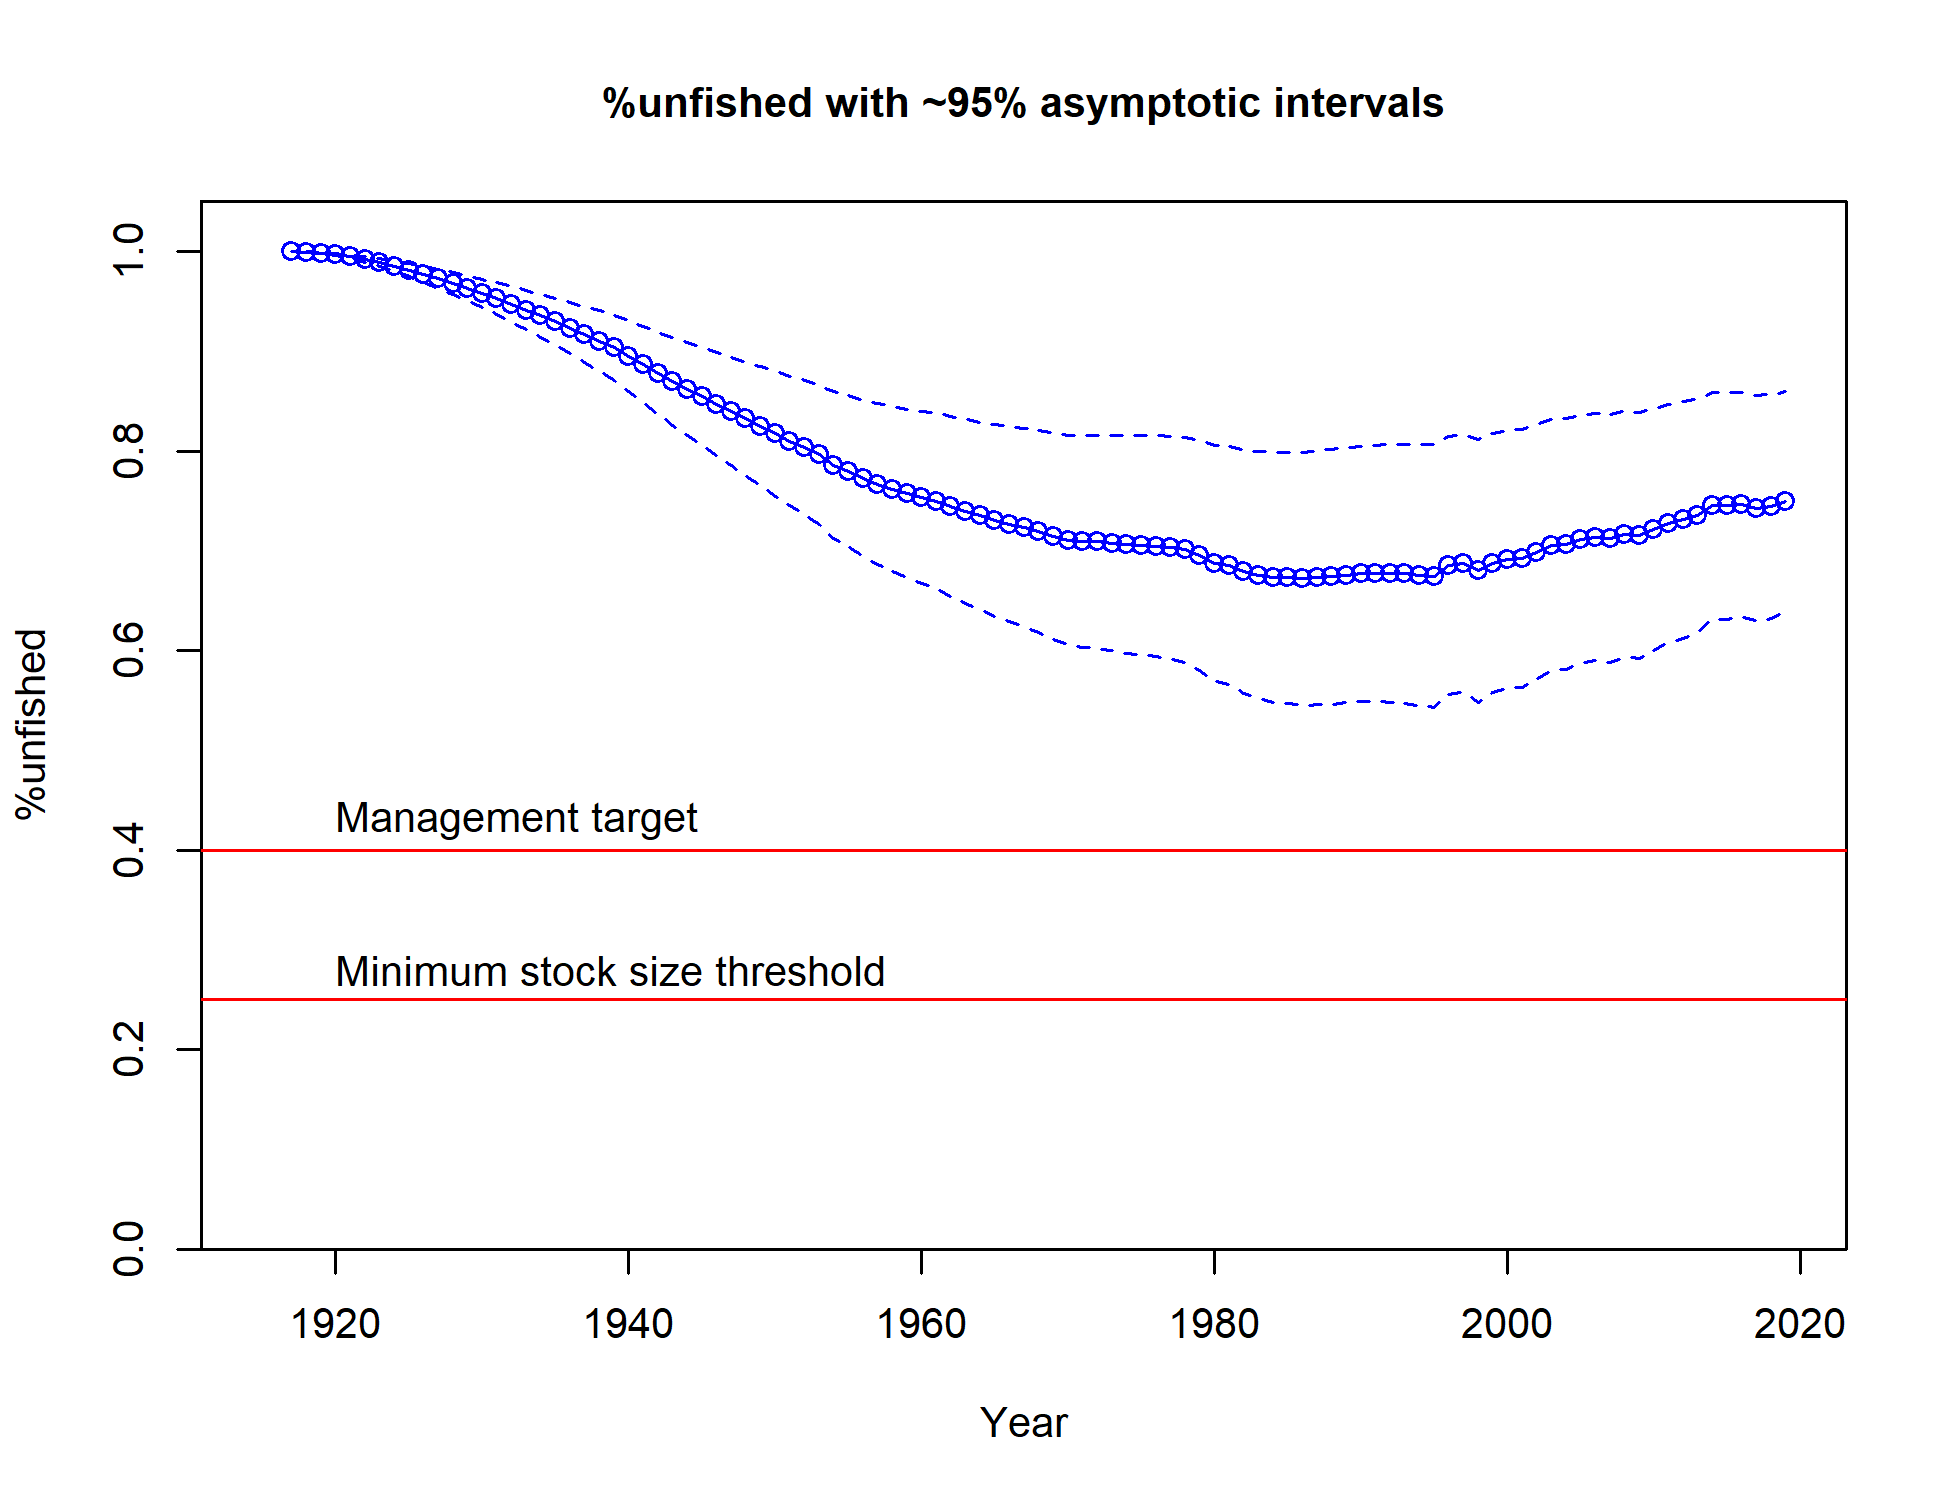
\includegraphics{r4ss/plots_mod1/ts9_Spawning_depletion_with_95_asymptotic_intervals_intervals.png}
\caption{Estimated relative depletion with approximate 95\% asymptotic
confidence intervals (dashed lines) for the base case assessment model.
\label{fig:RelDeplete_all}}
\end{figure}

\FloatBarrier

\hypertarget{recruitment}{%
\subsection*{Recruitment}\label{recruitment}}
\addcontentsline{toc}{subsection}{Recruitment}

Recruitment deviations were estimated from 1916-2018 (Figure
\ref{fig:Recruits_all} and Table \ref{tab:Recruit_mod1}).

\begin{table}[ht]
\centering
\caption{Recent recruitment for the model.} 
\label{tab:Recruit_mod1}
\begin{tabular}{>{\centering}p{.8in}>{\centering}p{1.6in}>{\centering}p{1.3in}}
  \hline
Year & Estimated Recruitment (1,000s) & \~{} 95\% confidence interval \\ 
  \hline
2010 & 3435.91 & (2128.69 - 5545.9) \\ 
  2011 & 3450.01 & (2142.11 - 5556.47) \\ 
  2012 & 3457.92 & (2149.79 - 5562.03) \\ 
  2013 & 3466.77 & (2158.45 - 5568.12) \\ 
  2014 & 3488.68 & (2179.48 - 5584.31) \\ 
  2015 & 3488.86 & (2180.18 - 5583.09) \\ 
  2016 & 3492.63 & (2184.26 - 5584.72) \\ 
  2017 & 3486.86 & (2179.33 - 5578.88) \\ 
  2018 & 3491.73 & (2184.37 - 5581.57) \\ 
  2019 & 3504.69 & (2186.12 - 5618.57) \\ 
   \hline
\end{tabular}
\end{table}

\FloatBarrier

\begin{figure}
\centering
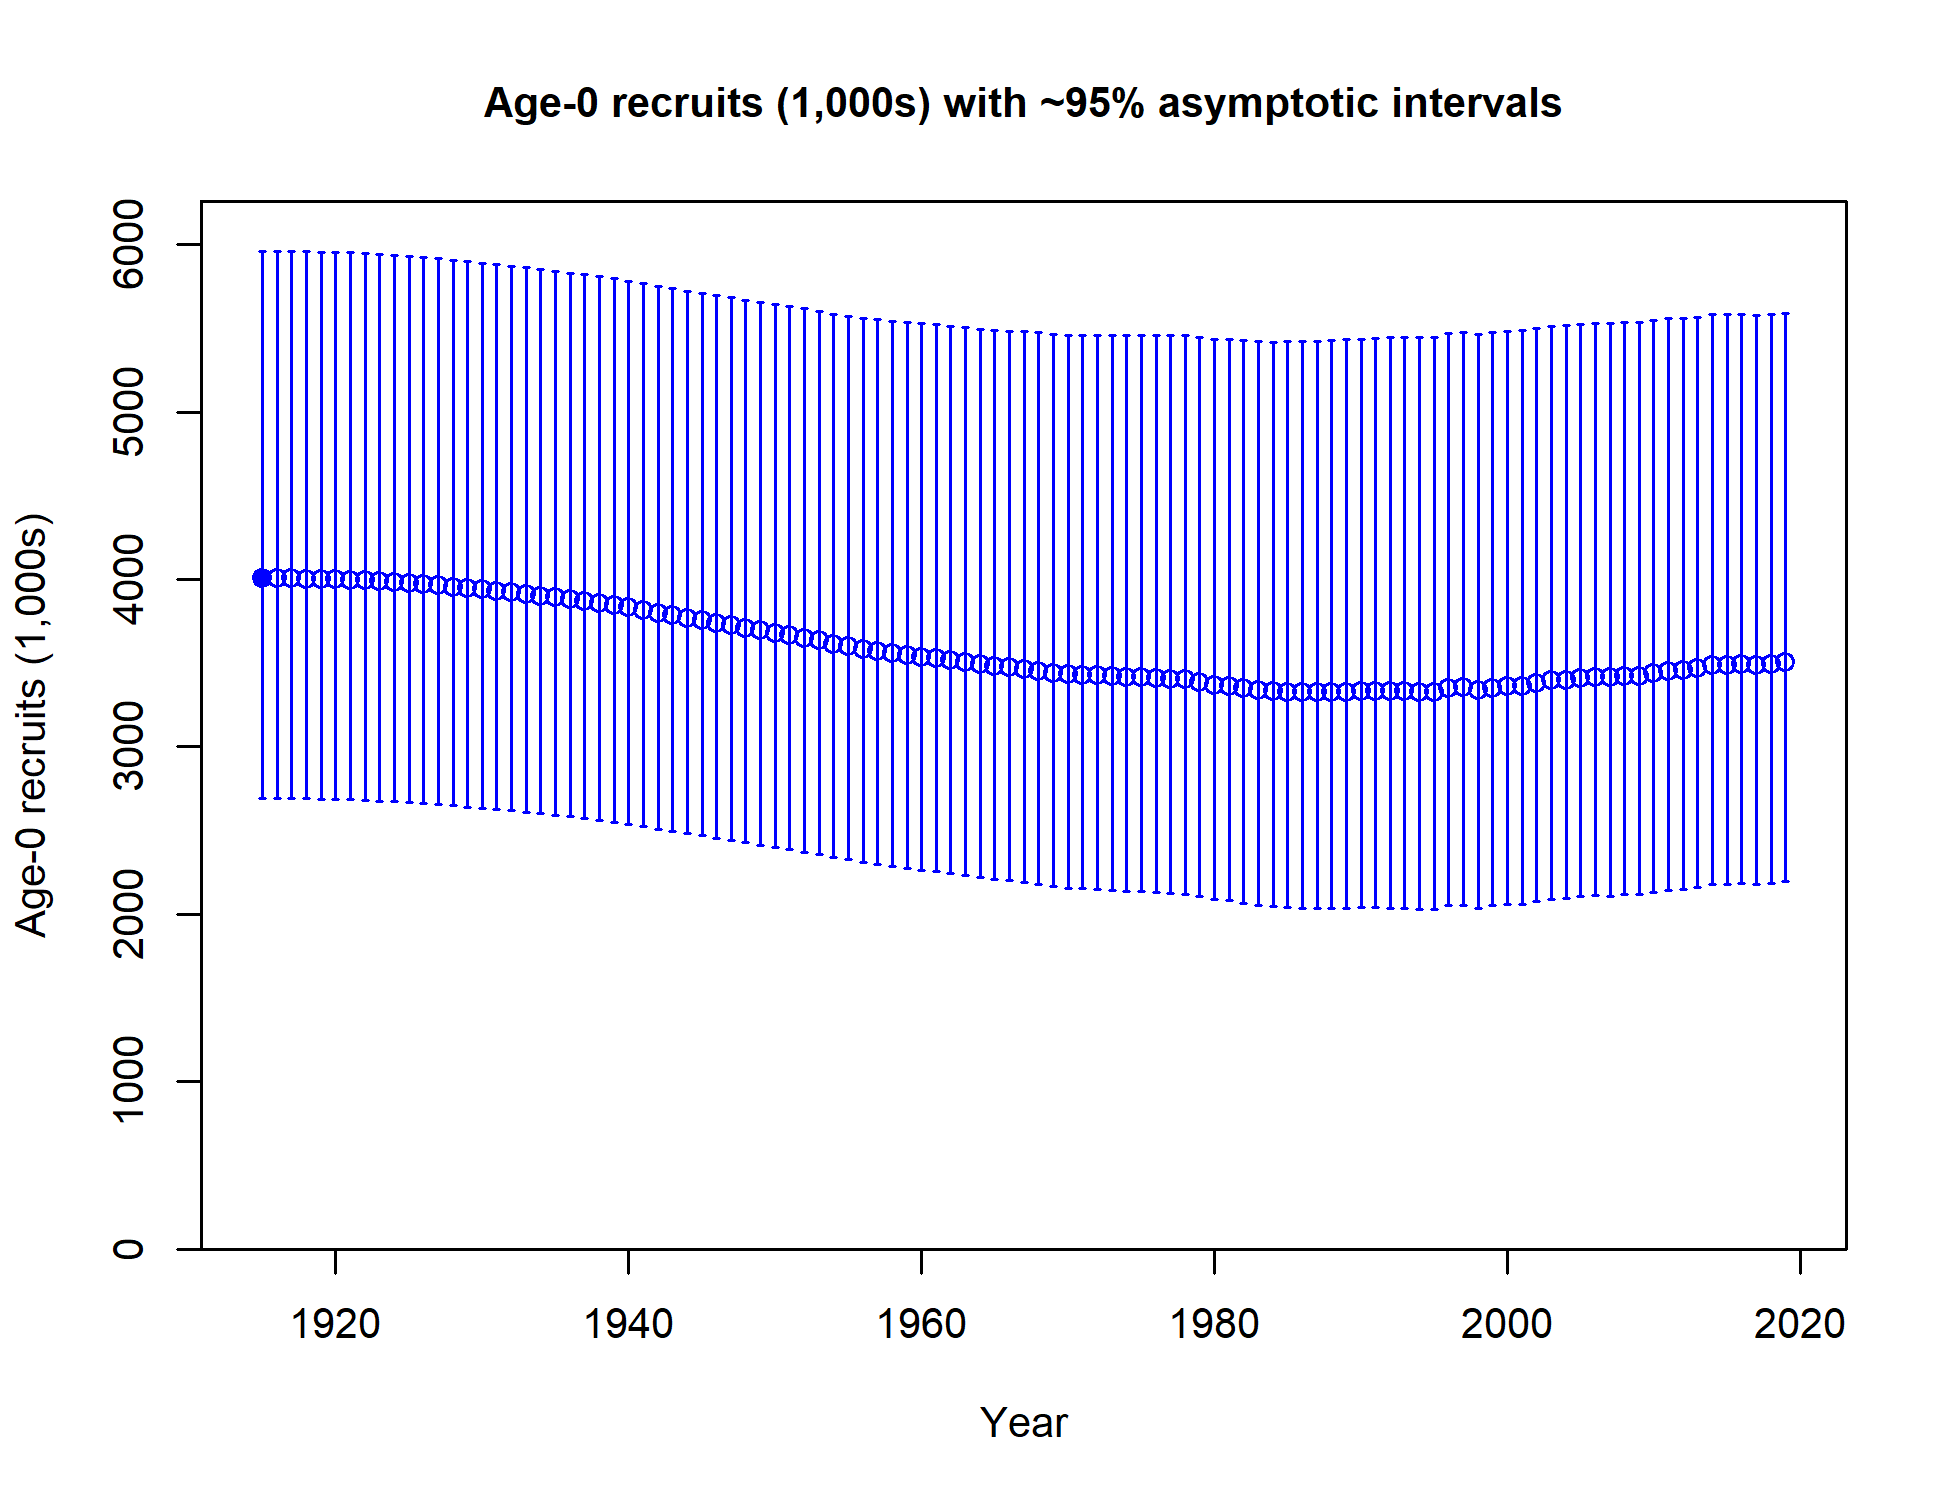
\includegraphics{r4ss/plots_mod1/ts11_Age-0_recruits_(1000s)_with_95_asymptotic_intervals.png}
\caption{Time series of estimated Big Skate recruitments for the
base-case model with 95\% confidence or credibility intervals.
\label{fig:Recruits_all}}
\end{figure}

\FloatBarrier

\hypertarget{exploitation-status}{%
\subsection*{Exploitation status}\label{exploitation-status}}
\addcontentsline{toc}{subsection}{Exploitation status}

Harvest rates estimated by the base model. management target levels
(Table \ref{tab:SPR_Exploit_mod1} and Figure \ref{fig:SPR_all}).

\FloatBarrier

\begin{table}[ht]
\centering
\caption{Recent trend in spawning potential 
                                        ratio and exploitation for Big Skate in the model.  Fishing intensity is (1-SPR) 
                                        divided by 50\% (the SPR target) and exploitation 
                                        is F divided by F\textsubscript{SPR}.} 
\label{tab:SPR_Exploit_mod1}
\begin{tabular}{l>{\centering}p{1in}>{\centering}p{1.2in}>{\centering}p{1in}>{\centering}p{1.2in}}
  \hline
Year & Fishing intensity & \~{} 95\% confidence interval & Exploitation rate & \~{} 95\% confidence interval \\ 
  \hline
2009 & 0.23 & (0.12-0.34) & 0.01 & (0.01-0.02) \\ 
  2010 & 0.22 & (0.11-0.32) & 0.01 & (0.01-0.02) \\ 
  2011 & 0.29 & (0.15-0.42) & 0.02 & (0.01-0.02) \\ 
  2012 & 0.29 & (0.15-0.42) & 0.02 & (0.01-0.02) \\ 
  2013 & 0.15 & (0.08-0.22) & 0.01 & (0-0.01) \\ 
  2014 & 0.39 & (0.22-0.56) & 0.02 & (0.01-0.03) \\ 
  2015 & 0.35 & (0.19-0.5) & 0.02 & (0.01-0.03) \\ 
  2016 & 0.43 & (0.24-0.61) & 0.02 & (0.01-0.04) \\ 
  2017 & 0.30 & (0.16-0.44) & 0.02 & (0.01-0.02) \\ 
  2018 & 0.19 & (0.1-0.28) & 0.01 & (0.01-0.01) \\ 
   \hline
\end{tabular}
\end{table}

\FloatBarrier

\begin{figure}
\centering
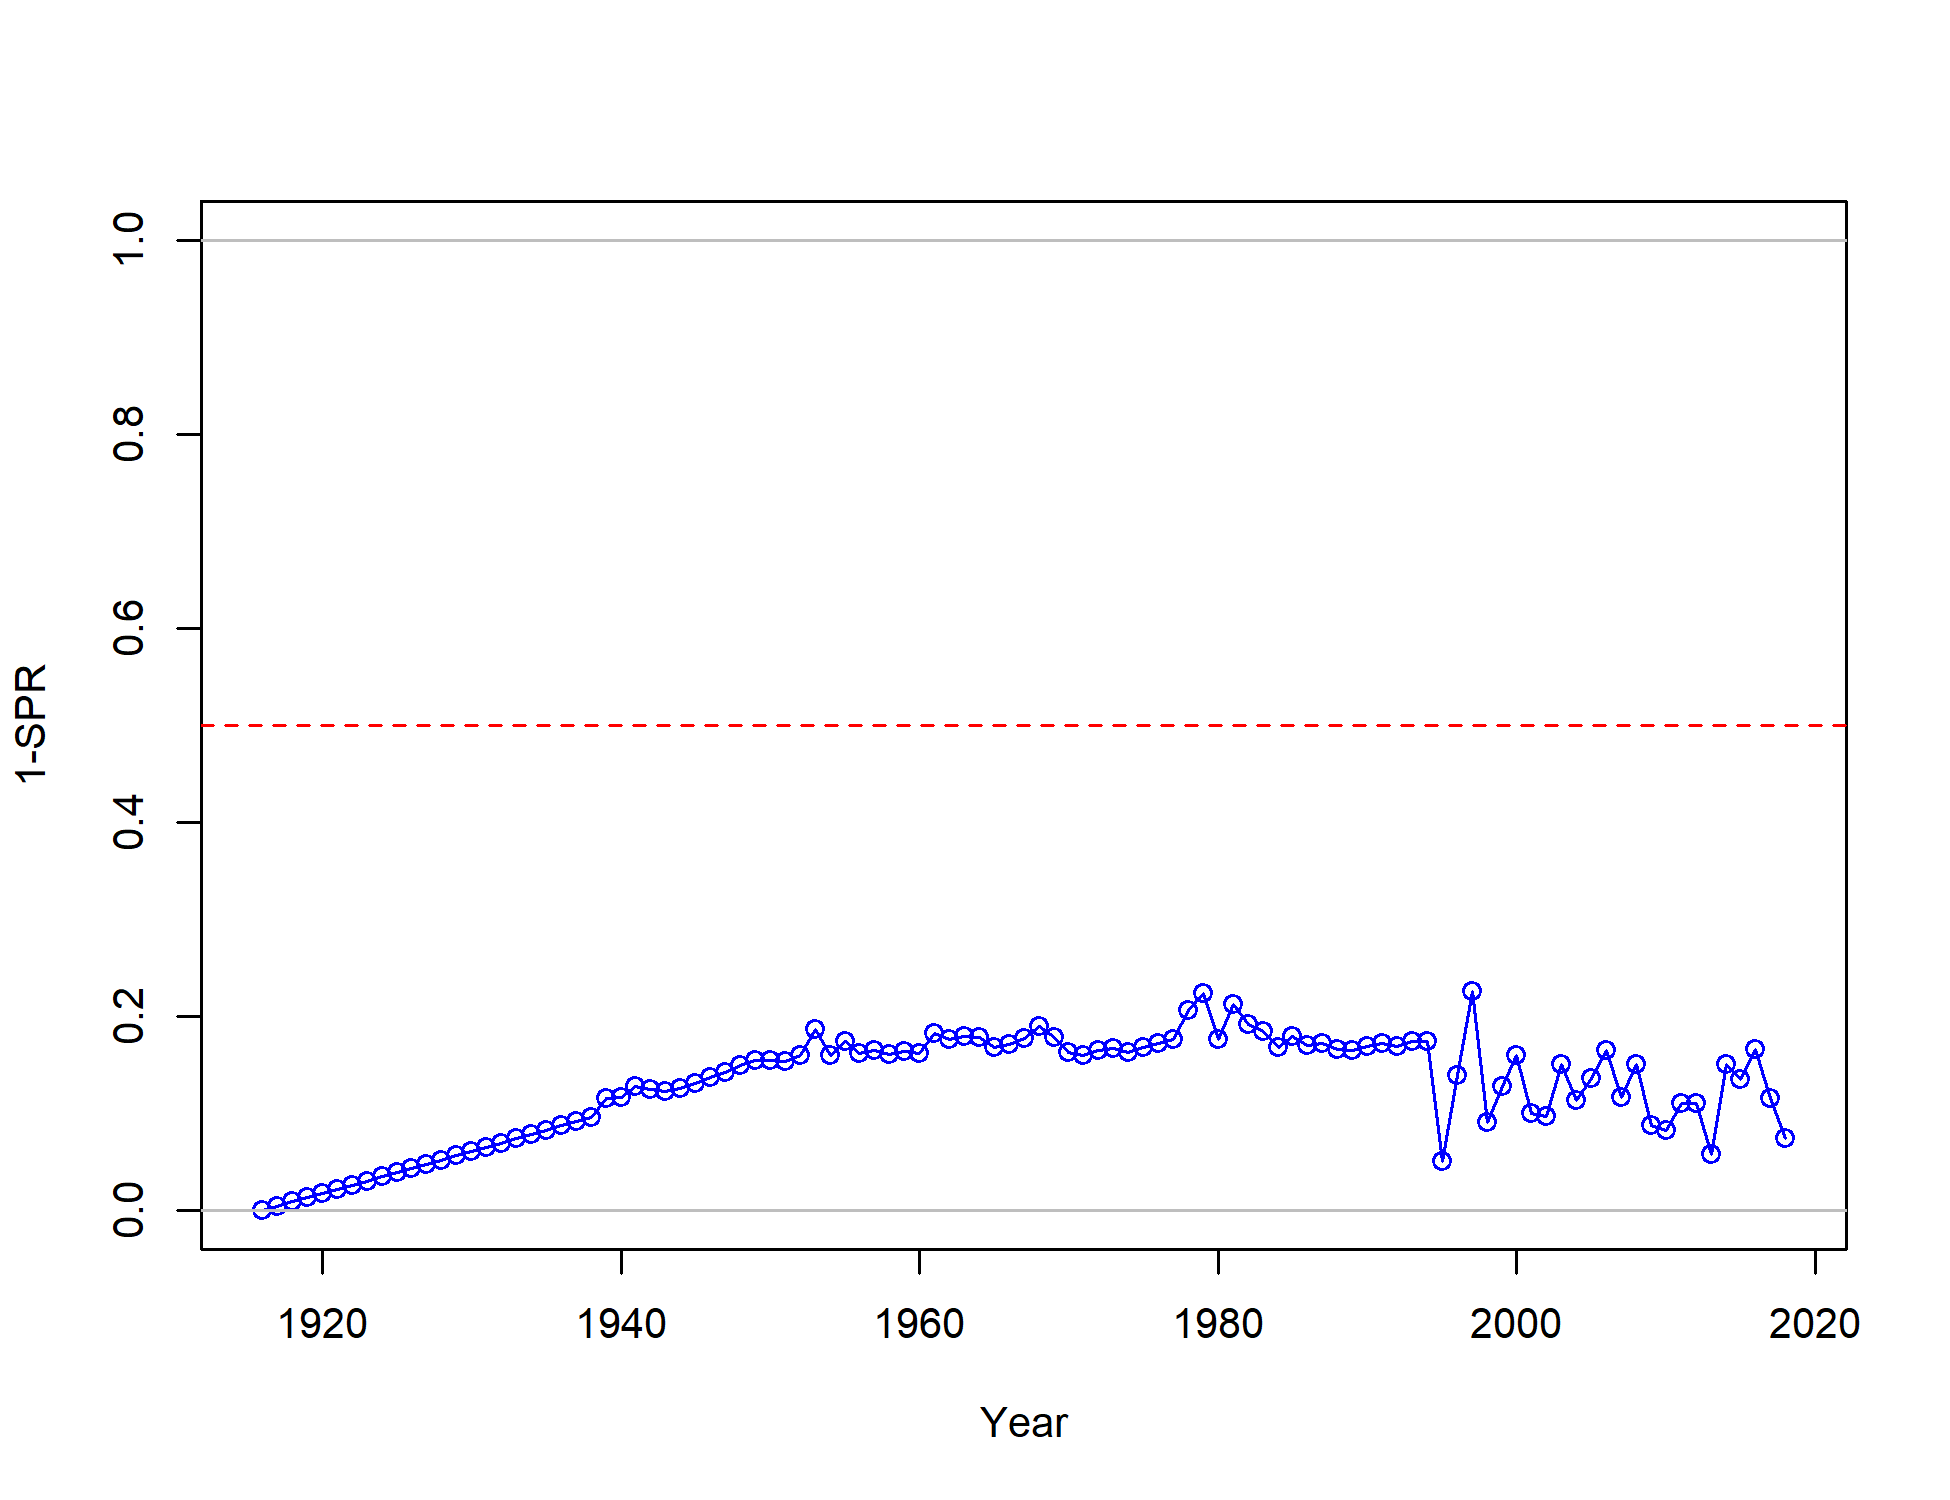
\includegraphics{r4ss/plots_mod1/SPR2_minusSPRseries.png}
\caption{Estimated spawning potential ratio (SPR) for the base-case
model. One minus SPR is plotted so that higher exploitation rates occur
on the upper portion of the y-axis. The management target is plotted as
a red horizontal line and values above this reflect harvests in excess
of the overfishing proxy based on the SPR\textsubscript{50\%} harvest
rate. The last year in the time series is 2018. \label{fig:SPR_all}}
\end{figure}

\FloatBarrier

\hypertarget{ecosystem-considerations}{%
\subsection*{Ecosystem Considerations}\label{ecosystem-considerations}}
\addcontentsline{toc}{subsection}{Ecosystem Considerations}

In this assessment, ecosystem considerations were not explicitly
included in the analysis.\\
This is primarily due to a lack of relevant data and results of analyses
(conducted elsewhere) that could contribute ecosystem-related
quantitative information for the assessment.

\hypertarget{reference-points}\)), and well above the minimum stock size
threshold (\(SB_{25\%}\)). The estimated relative depletion level for
the base model in 2019 is 72.5\% (95\% asymptotic interval: \(\pm\)
55.2\%-89.7\%, corresponding to an unfished spawning biomass of 1106.07
million eggs (95\% asymptotic interval: 504.33-1707.81 million eggs) of
spawning biomass in the base model (Table \ref{tab:Ref_pts_mod1}).
Unfished age 1+ biomass was estimated to be 2,426 mt in the base case
model. The target spawning biomass (\(SB_{40\%}\)) is 610 million eggs,
which corresponds with an equilibrium yield of 558 mt. Equilibrium yield
at the proxy \(F_{MSY}\) harvest rate corresponding to \(SPR_{50\%}\) is
466 mt (Figure \ref{fig:Yield_all}).

\FloatBarrier

\begin{table}[ht]
\centering
\caption{Summary of reference 
                                      points and management quantities for the 
                                      base case model.} 
\label{tab:Ref_pts_mod1}
\begin{tabular}{>{\raggedright}p{4.1in}>{\raggedleft}p{.62in}>{\raggedleft}p{.62in}>{\raggedleft}p{.62in}}
  \hline
\textbf{Quantity} & \textbf{Estimate} & \textbf{Low 2.5\%  limit} & \textbf{High 2.5\%  limit} \\ 
  \hline
Unfished spawning output (million eggs) & 1,526 & 891 & 2,161 \\ 
  Unfished age 1+ biomass (mt) & 2,426 & 1,583 & 3,269 \\ 
  Unfished recruitment ($R_{0}$) & 4,004 & 2,395 & 5,612 \\ 
  Spawning output(2018 million eggs) & 1,097 & 462 & 1,732 \\ 
  Depletion (2018) & 0.719 & 0.586 & 0.852 \\ 
  \textbf{$\text{Reference points based on } \mathbf{SB_{40\%}}$} &  &  &  \\ 
  Proxy spawning output ($B_{40\%}$) & 610 & 373 & 848 \\ 
  SPR resulting in $B_{40\%}$ ($SPR_{B40\%}$) & 0.625 & 0.625 & 0.625 \\ 
  Exploitation rate resulting in $B_{40\%}$ & 0.047 & 0.043 & 0.051 \\ 
  Yield with $SPR_{B40\%}$ at $B_{40\%}$ (mt) & 558 & 362 & 754 \\ 
  \textbf{\textit{Reference points based on SPR proxy for MSY}} &  &  &  \\ 
  Spawning output & 305 & 187 & 424 \\ 
  $SPR_{proxy}$ & 0.5 &  &  \\ 
  Exploitation rate corresponding to $SPR_{proxy}$ & 0.069 & 0.063 & 0.075 \\ 
  Yield with $SPR_{proxy}$ at $SB_{SPR}$ (mt) & 466 & 303 & 629 \\ 
  \textbf{\textit{Reference points based on estimated MSY values}} &  &  &  \\ 
  Spawning output at $MSY$ ($SB_{MSY}$) & 578 & 352 & 804 \\ 
  $SPR_{MSY}$ & 0.612 & 0.608 & 0.615 \\ 
  Exploitation rate at $MSY$ & 0.049 & 0.045 & 0.053 \\ 
  Dead Catch $MSY$ (mt) & 559 & 363 & 755 \\ 
  Retained Catch $MSY$ (mt) & 517 & 337 & 698 \\ 
   \hline
\end{tabular}
\end{table}

\FloatBarrier

\hypertarget{management-performance}{%
\subsection*{Management Performance}\label{management-performance}}
\addcontentsline{toc}{subsection}{Management Performance}

Table \ref{tab:mnmgt_perform}

\begin{table}[ht]
\centering
\caption{Recent trend in total catch (mt) relative to the 
                              management guidelines. Big skate was
                              managed in the Other Species complex in 2013 and 2014,
                              designated an Ecosystem Component species in 2015 and
                              2016, and managed with stock-specific harvest
                              specifications since 2017.} 
\label{tab:mnmgt_perform}
\scalebox{0.9}{
\begin{tabular}{>{\raggedleft}p{1in}>{\centering}p{1in}>{\centering}p{1in}>{\centering}p{1in}>{\centering}p{1in}}
  \hline
Year & OFL (mt; ABC prior to 2011) & ABC (mt) & ACL (mt; OY prior to 2011) & Estimated total catch (mt) \\ 
  \hline
\textbf{2009} &  &  &  & 205.70 \\ 
  \textbf{2010} &  &  &  & 196.20 \\ 
  \textbf{2011} &  &  &  & 268.40 \\ 
  \textbf{2012} &  &  &  & 269.60 \\ 
  \textbf{2013} & 458.00 & 317.90 & 317.90 & 135.00 \\ 
  \textbf{2014} & 458.00 & 317.90 & 317.90 & 372.40 \\ 
  \textbf{2015} &  &  &  & 331.50 \\ 
  \textbf{2016} &  &  &  & 411.50 \\ 
  \textbf{2017} & 541.00 & 494.00 & 494.00 & 277.60 \\ 
  \textbf{2018} & 541.00 & 494.00 & 494.00 & 172.60 \\ 
  \textbf{2019} & 541.00 & 494.00 & 494.00 &  \\ 
  \textbf{2020} & 541.00 & 494.00 & 494.00 &  \\ 
   \hline
\end{tabular}
}
\end{table}

\hypertarget{unresolved-problems-and-major-uncertainties}{%
\subsection*{Unresolved Problems and Major
Uncertainties}\label{unresolved-problems-and-major-uncertainties}}
\addcontentsline{toc}{subsection}{Unresolved Problems and Major
Uncertainties}

\FloatBarrier

\hypertarget{decision-table}{%
\subsection*{Decision Table}\label{decision-table}}
\addcontentsline{toc}{subsection}{Decision Table}

\begin{table}[ht]
\centering
\caption{Projections of potential OFL (mt) for 
                                        each model, using the base model forecast.} 
\label{tab:OFL_projection}
\begin{tabular}{lr}
  \hline
Year & OFL \\ 
  \hline
2019 & 1274.29 \\ 
  2020 & 1211.22 \\ 
  2021 & 1159.12 \\ 
  2022 & 1117.47 \\ 
  2023 & 1083.86 \\ 
  2024 & 1055.15 \\ 
  2025 & 1029.12 \\ 
  2026 & 1004.39 \\ 
  2027 & 980.33 \\ 
  2028 & 956.75 \\ 
  2029 & 933.76 \\ 
  2030 & 911.62 \\ 
   \hline
\end{tabular}
\end{table}
\begin{table}[ht]
\centering
\caption{Summary of 10-year 
                                             projections beginning in 2020 
                                             for alternate states of nature based on 
                                             an axis of uncertainty for the model.  Columns range over low, mid, and high
                                             states of nature, and rows range over different 
                                             assumptions of catch levels. An entry of "--" 
                                             indicates that the stock is driven to very low 
                                             abundance under the particular scenario.} 
\label{tab:Decision_table_mod1}
\scalebox{0.85}{
\begin{tabular}{l|cc|>{\centering}p{.7in}c|>{\centering}p{.7in}c|>{\centering}p{.7in}c}
   \multicolumn{3}{c}{}  &  \multicolumn{2}{c}{} 
                               & \multicolumn{2}{c}{\textbf{States of nature}} 
                               & \multicolumn{2}{c}{} \\
  \multicolumn{3}{c}{}  &  \multicolumn{2}{c}{Low M 0.05} 
                               & \multicolumn{2}{c}{Base M 0.07} 
                               &  \multicolumn{2}{c}{High M 0.09} \\
 \hline
 & Year & Catch & Spawning Output & Depletion & Spawning Output & Depletion & Spawning Output & Depletion \\ 
  \hline
 & 2019 & - & - & - & - & - & - & - \\ 
   & 2020 & - & - & - & - & - & - & - \\ 
   & 2021 & - & - & - & - & - & - & - \\ 
  40-10 Rule,  & 2022 & - & - & - & - & - & - & - \\ 
  Low M & 2023 & - & - & - & - & - & - & - \\ 
   & 2024 & - & - & - & - & - & - & - \\ 
   & 2025 & - & - & - & - & - & - & - \\ 
   & 2026 & - & - & - & - & - & - & - \\ 
   & 2027 & - & - & - & - & - & - & - \\ 
   & 2028 & - & - & - & - & - & - & - \\ 
   \hline
 & 2019 & - & - & - & - & - & - & - \\ 
   & 2020 & - & - & - & - & - & - & - \\ 
   & 2021 & - & - & - & - & - & - & - \\ 
  40-10 Rule & 2022 & - & - & - & - & - & - & - \\ 
   & 2023 & - & - & - & - & - & - & - \\ 
   & 2024 & - & - & - & - & - & - & - \\ 
   & 2025 & - & - & - & - & - & - & - \\ 
   & 2026 & - & - & - & - & - & - & - \\ 
   & 2027 & - & - & - & - & - & - & - \\ 
   & 2028 & - & - & - & - & - & - & - \\ 
   \hline
 & 2019 & - & - & - & - & - & - & - \\ 
   & 2020 & - & - & - & - & - & - & - \\ 
   & 2021 & - & - & - & - & - & - & - \\ 
  40-10 Rule, & 2022 & - & - & - & - & - & - & - \\ 
  High M & 2023 & - & - & - & - & - & - & - \\ 
   & 2024 & - & - & - & - & - & - & - \\ 
   & 2025 & - & - & - & - & - & - & - \\ 
   & 2026 & - & - & - & - & - & - & - \\ 
   & 2027 & - & - & - & - & - & - & - \\ 
   & 2028 & - & - & - & - & - & - & - \\ 
   \hline
 & 2019 & - & - & - & - & - & - & - \\ 
   & 2020 & - & - & - & - & - & - & - \\ 
   & 2021 & - & - & - & - & - & - & - \\ 
  Average & 2022 & - & - & - & - & - & - & - \\ 
  Catch & 2023 & - & - & - & - & - & - & - \\ 
   & 2024 & - & - & - & - & - & - & - \\ 
   & 2025 & - & - & - & - & - & - & - \\ 
   & 2026 & - & - & - & - & - & - & - \\ 
   & 2027 & - & - & - & - & - & - & - \\ 
   & 2028 & - & - & - & - & - & - & - \\ 
   \hline
\end{tabular}
}
\end{table}

\begin{sidewaystable}[ht]
\centering
\caption{Base case results summary.} 
\label{tab:base_summary}
\scalebox{0.6}{
\begin{tabular}{r>{\centering}p{1.1in}>{\centering}p{1.1in}>{\centering}p{1.1in}>{\centering}p{1.1in}>{\centering}p{1.1in}>{\centering}p{1.1in}>{\centering}p{1.1in}>{\centering}p{1.1in}>{\centering}p{1.1in}>{\centering}p{1.1in}}
  \hline
Quantity & 2010 & 2011 & 2012 & 2013 & 2014 & 2015 & 2016 & 2017 & 2018 & 2019 \\ 
  \hline
Landings (mt) &  &  &  &  &  &  &  &  &  &  \\ 
  Total Est. Catch (mt) &  &  &  &  &  &  &  &  &  &  \\ 
  OFL (mt) &  &  &  &  &  &  &  &  &  &  \\ 
  ACL (mt) &  &  &  &  &  &  &  &  &  &  \\ 
   \hline
(1-$SPR$)(1-$SPR_{50\%}$) & 0.22 & 0.29 & 0.29 & 0.15 & 0.39 & 0.35 & 0.43 & 0.30 & 0.19 &  \\ 
   \hline
Exploitation rate & 0.01 & 0.02 & 0.02 & 0.01 & 0.02 & 0.02 & 0.02 & 0.02 & 0.01 &  \\ 
  Age 1+ biomass (mt) & 17752.6 & 17914.2 & 18070.4 & 18140.7 & 18203.3 & 18389.4 & 18320.0 & 18306.6 & 18214.4 & 18273.9 \\ 
   \hline
Spawning Output & 1059.2 & 1068.7 & 1074.0 & 1080.0 & 1095.0 & 1095.1 & 1097.7 & 1093.7 & 1097.1 & 1106.1 \\ 
  ~95\% CI & (425.78-1692.72) & (434.08-1703.26) & (438.95-1709.03) & (444.55-1715.41) & (458.25-1731.69) & (458.91-1731.29) & (461.69-1733.71) & (458.52-1728.92) & (461.78-1732.38) & (504.33-1707.81) \\ 
   \hline
Depletion & 0.7 & 0.7 & 0.7 & 0.7 & 0.7 & 0.7 & 0.7 & 0.7 & 0.7 & 0.7 \\ 
  ~95\% CI & (0.552-0.837) & (0.56-0.841) & (0.564-0.843) & (0.57-0.846) & (0.583-0.852) & (0.583-0.852) & (0.586-0.853) & (0.583-0.851) & (0.586-0.852) & (0.552-0.897) \\ 
   \hline
Recruits & 3435.91 & 3450.01 & 3457.92 & 3466.77 & 3488.68 & 3488.86 & 3492.63 & 3486.86 & 3491.73 & 3504.69 \\ 
  ~95\% CI & (2128.69 - 5545.9) & (2142.11 - 5556.47) & (2149.79 - 5562.03) & (2158.45 - 5568.12) & (2179.48 - 5584.31) & (2180.18 - 5583.09) & (2184.26 - 5584.72) & (2179.33 - 5578.88) & (2184.37 - 5581.57) & (2186.12 - 5618.57) \\ 
   \hline
\end{tabular}
}
\end{sidewaystable}

\begin{figure}
\centering
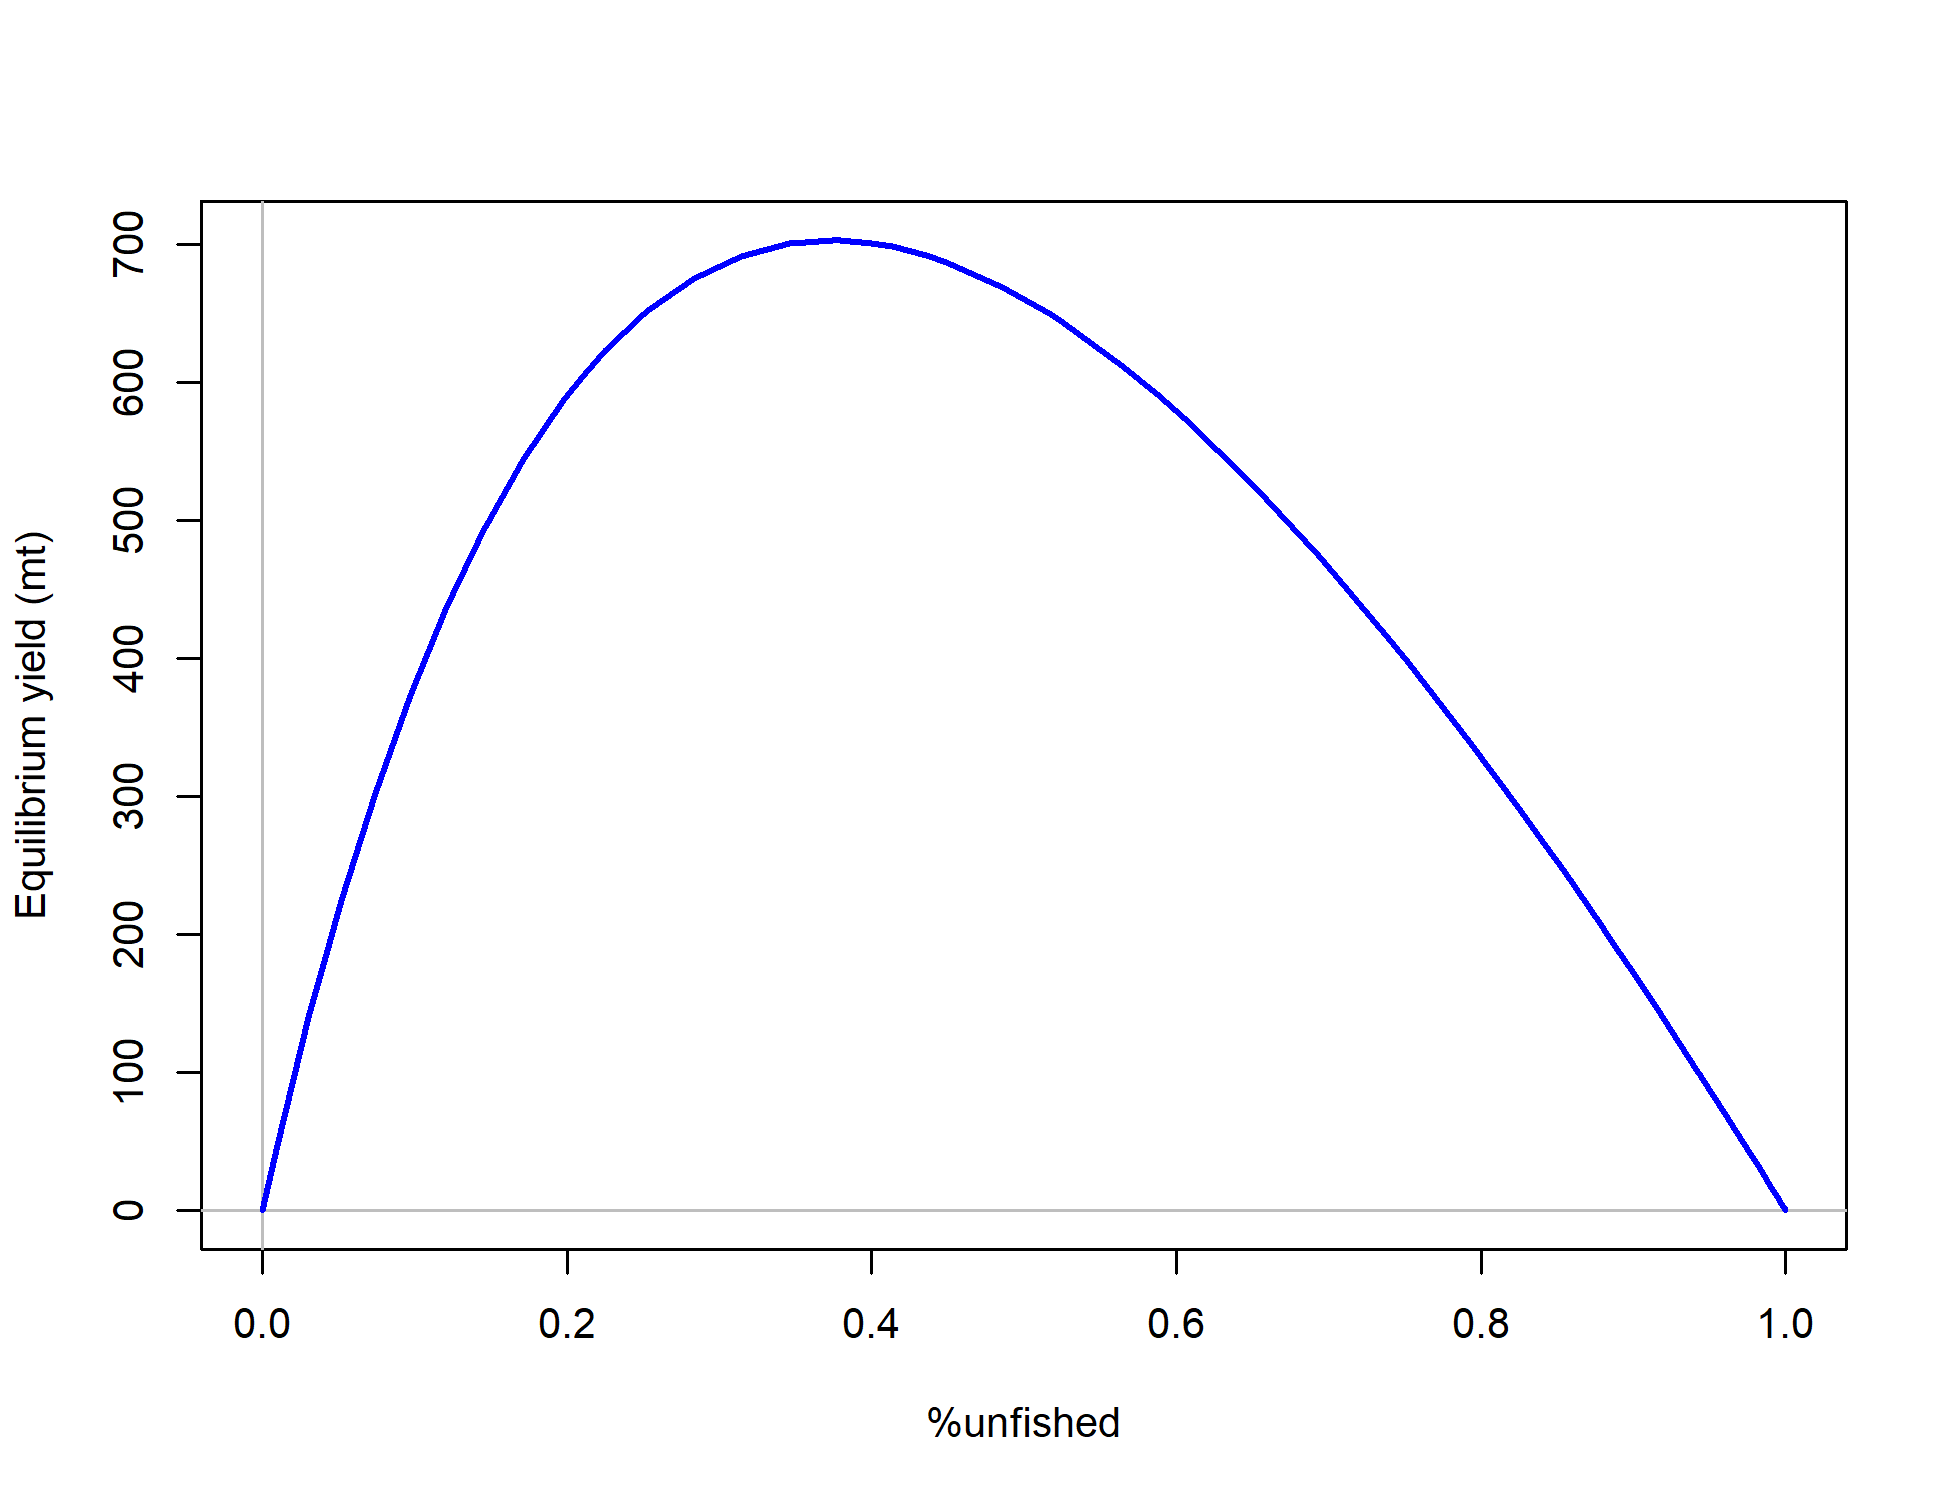
\includegraphics{r4ss/plots_mod1/yield1_yield_curve.png}
\caption{Equilibrium yield curve for the base case model. Values are
based on the 2018 fishery selectivity and with steepness fixed at 0.718.
\label{fig:Yield_all}}
\end{figure}

\FloatBarrier

\newpage

\hypertarget{research-and-data-needs}{%
\subsection*{Research and Data Needs}\label{research-and-data-needs}}
\addcontentsline{toc}{subsection}{Research and Data Needs}

We recommend the following research be conducted before the next
assessment:

\begin{enumerate}

\item \textbf{xxxx}: 

\item \textbf{xxxx}:

\item \textbf{xxxx}:

\item \textbf{xxxx}:

\item \textbf{xxxx}:

\end{enumerate}

\FloatBarrier

\newpage
\renewcommand{\thefigure}{\arabic{figure}}
\renewcommand{\thetable}{\arabic{table}}
\setcounter{figure}{0}
\setcounter{table}{0}

\newpage
\renewcommand{\thefigure}{\arabic{figure}}
\renewcommand{\thetable}{\arabic{table}}
\setcounter{figure}{0}
\setcounter{table}{0}

\hypertarget{introduction}{%
\section{Introduction}\label{introduction}}

\hypertarget{distribution-and-life-history}{%
\subsection{Distribution and Life
History}\label{distribution-and-life-history}}

Skates are the largest and most widely distributed group of batoid fish
with approximately 245 species ascribed to two families (Ebert and
Compagno (\protect\hyperlink{ref-Ebert2007}{2007}), McEachran and Miyake
(\protect\hyperlink{ref-McEachran1990}{1990})). Skates are benthic fish
that are found in all coastal waters but are most common in cold
temperatures and polar waters (Ebert and Compagno
\protect\hyperlink{ref-Ebert2007}{2007}).

There are eleven species of skates in three genera (Amblyraja,
Bathyraja, and Raja) present in the Northeast Pacific Ocean off
California, Oregon and Washington (Ebert 2003). Of that number, just
three species (Longnose Skate, \emph{Raja rhina}; Big Skate, \emph{Raja
binoculata}; and Sandpaper Skate, \emph{Bathyraja interrupta}) make up
over 95 percent of West Coast Groundfish Bottom Trawl Survey (WCGBTS)
catches in terms of biomass and numbers, with the Longnose Skate leading
in both categories (with 62 percent of biomass and 56 percent of
numbers).

Big Skate (\emph{Raja binoculata}) is the largest of the skate species
in North America with a documented maximum length of 244 cm total length
and a maximum weight of 91 kg (Eschmeyer and Herald
\protect\hyperlink{ref-Eschmeyer1983}{1983}). The species name
``binoculata'' (two-eyed) refers to the prominent ocellus at the base of
each pectoral fin. Big Skates are usually seen buried in sediment with
only their eyes showing.

The Big Skate is most common in soft-sediment habitats in coastal waters
of the continental shelf (Bizzarro, JJ and Broms, KM and Logsdon, MG and
Ebert, DA and Yoklavich, MM and Kuhnz, LA and Summers, AP
(\protect\hyperlink{ref-Bizzarro2014}{2014}), Farrugia et al.
(\protect\hyperlink{ref-Farrugia2016}{2016})). Use of mixed substrate
(e.g., mud with boulders) increases with ontogeny but hard substrates
are largely avoided (Bizzarro
(\protect\hyperlink{ref-Bizzarro2015}{2015})). In the GOA, the Big Skate
is the most commonly encountered skate species in continental shelf
waters at 100--200 m depth, and is most abundant in the central and
western areas of the GOA (Stevenson, DE and Orr, JW and Hoff, GR and
McEachran, JD (\protect\hyperlink{ref-Stevenson2008}{2008}); Bizzarro,
JJ and Broms, KM and Logsdon, MG and Ebert, DA and Yoklavich, MM and
Kuhnz, LA and Summers, AP (\protect\hyperlink{ref-Bizzarro2014}{2014})).
Off the U.S. Pacific Coast, the Big Skate is most densely distributed on
the inner continental shelf (\textless{} 100 m; Bizzarro, JJ and Broms,
KM and Logsdon, MG and Ebert, DA and Yoklavich, MM and Kuhnz, LA and
Summers, AP (\protect\hyperlink{ref-Bizzarro2014}{2014})). Eggs are
mainly deposited between 70--90 m on sand or mud substrates (Hitz
(\protect\hyperlink{ref-Hitz1964}{1964}); NMFS-NWFSC-FRAM, unpub. data).
Juveniles typically occur in shallower waters than adults (Bizzarro
(\protect\hyperlink{ref-Bizzarro2015}{2015})). Core habitat regions of
Big Skate off the U.S. Pacific Coast and in the Gulf of Alaska are
spatially segregated from those of other species (Bizzarro, JJ and
Broms, KM and Logsdon, MG and Ebert, DA and Yoklavich, MM and Kuhnz, LA
and Summers, AP (\protect\hyperlink{ref-Bizzarro2014}{2014})).

Big Skates are highly mobile and capable of long range (\textgreater{}
2000 km) movements (KingandMcF2010; Farrugia et al.
(\protect\hyperlink{ref-Farrugia2016}{2016})). For example, in British
Columbia, a study revealed that \textasciitilde{}75\% of tagged
individuals were recaptured within 21 km of the tagging locations, but
15 of the tagged individuals (0.1\%) moved over 1,000 km (max = 2340 km;
King, JR and McFarlane, GA
(\protect\hyperlink{ref-KingandMcF2010}{2010})). In the Gulf of Alaska,
a year of satellite tag data showed that six of twelve tagged
individuals moved over 100 km, with one skate moving \textgreater{}
2,000 km (Farrugia et al.~2016). Although primarily benthic, Big Skates
utilize the entire water column including surface waters (Farrugia et
al. (\protect\hyperlink{ref-Farrugia2016}{2016})). They have broad
thermal tolerances 2--19º C that enable their occurrence from boreal to
subtropical latitudes (Love, Milton S
(\protect\hyperlink{ref-Love2011}{2011}); Farrugia et al.
(\protect\hyperlink{ref-Farrugia2016}{2016})).

Big Skates are opportunistic, generalist mesopredators with highly
variable spatio-temporal trophic roles (Ebert and Compagno
(\protect\hyperlink{ref-Ebert2007}{2007}); Bizzarro
(\protect\hyperlink{ref-Bizzarro2015}{2015})). Off central California,
diet of Big Skates is composed mainly of fishes, shrimps, and crabs (in
descending order), with larger skates incorporating more fishes
(({\textbf{???}})); however, in the Gulf of Alaska, Big Skate diet
consists mainly of crabs (esp.~Tanner Crabs) throughout ontogeny, with
relatively small portions of fishes and shrimps (Bizzarro
(\protect\hyperlink{ref-Bizzarro2015}{2015})). Correspondingly, trophic
level and general diet composition estimates differ significantly
between California and Gulf of Alaska Big Skate populations (Bizzarro
(\protect\hyperlink{ref-Bizzarro2015}{2015})).

Big Skates and their egg cases are preyed upon by a variety of
vertebrates and invertebrates. Snails and other molluscs bore holes in
egg cases to feed on developing embryos and especially their protein
rich yolk-sacs (Bizzarro, pers. obs; Hoff, GR
(\protect\hyperlink{ref-Hoff2009}{2009})). Sevengill Sharks, Brown
Rockfish, and Stellar Sea Lions are known predators of juvenile and
adult Big Skates (Ebert (\protect\hyperlink{ref-Ebert2003}{2003}), Love,
Milton S (\protect\hyperlink{ref-Love2011}{2011})). Northern Sea Lions
consume free-living Big Skates and their egg cases (Ebert
(\protect\hyperlink{ref-Ebert2003}{2003}), Love, Milton S
(\protect\hyperlink{ref-Love2011}{2011})).

In 2012, the Big Skate was moved from genus \emph{Raja} to the new genus
\emph{Beringraja} together with the Mottled Skate (\emph{B. pulchra})
(Ishihara et al. \protect\hyperlink{ref-Ishihara2012}{2012}). These are
the only two skates with multiple embryos per egg case, and they are
very similar mophologically and genetically (Bizzarro, J.
\protect\hyperlink{ref-Bizzarro2019}{2019}).

\hypertarget{biology}{%
\subsection{Biology}\label{biology}}

The Big Skate is broadly distributed, occurring from the southeastern
Bering Sea (Mecklenburg, CW and Mecklenburg, TA and Thorsteinson, LK
\protect\hyperlink{ref-Mecklenburg2002}{2002}) to southern Baja
California (22.90º N, 110.03º W; (Castro-Aguirre et al.
\protect\hyperlink{ref-Castro1993}{1993})) and the Gulf of California
(Castro-Aguirre and Pérez \protect\hyperlink{ref-Castro1996}{1996}). It
has been reported at depths of 2--501 m (min: Miller et al.
(\protect\hyperlink{ref-Miller1980}{1980}); max: Farrugia et al.
(\protect\hyperlink{ref-Farrugia2016}{2016})) but is most common on the
inner continental shelf (\textless{} 100 m; (Love, Milton S
\protect\hyperlink{ref-Love2011}{2011}); (Bizzarro
\protect\hyperlink{ref-Bizzarro2015}{2015})). Big Skates are highly
mobile and capable of long range (\textgreater{} 2000 km) movements
((King and McFarlane \protect\hyperlink{ref-KingandMcF2009}{2009});
(Farrugia et al. \protect\hyperlink{ref-Farrugia2016}{2016})).

Big Skate is oviparious, and is one of two skate species that have
multiple embryos per egg case (Ebert et al.
\protect\hyperlink{ref-Ebert2008}{2008}). From 1--8 embryos can be
contained in a single, large egg capsule, but most have 3--4 (DeLacy and
Chapman \protect\hyperlink{ref-DeLacy1935}{1935}, Hitz
\protect\hyperlink{ref-Hitz1964}{1964}, Ford
\protect\hyperlink{ref-Ford1971}{1971}). Eggs are deposited year-round
on sand or mud substrates at depths of \textasciitilde{}50--150 m (Hitz
\protect\hyperlink{ref-Hitz1964}{1964}, Ebert and Compagno
\protect\hyperlink{ref-Ebert2007}{2007}). Embryos hatch from eggs after
6--20 months, with shorter developmental periods associated with warmer
temperatures (Hoff, GR \protect\hyperlink{ref-Hoff2009}{2009}). In
captivity, Big Skate females may produce \textgreater{} 350 eggs/year
(average of 2 embryos/egg case; Chiquillo, Kelcie L and Ebert, David A
and Slager, Christina J and Crow, Karen D
(\protect\hyperlink{ref-Chiquillo2014}{2014})) from long-term sperm
storage ({\textbf{???}}). Size at birth is 18--23 cm TL (Ebert
\protect\hyperlink{ref-Ebert2003}{2003}). Maximum size is 244 cm TL
{[}Eschmeyer and Herald (\protect\hyperlink{ref-Eschmeyer1983}{1983}),
with females growing to larger sizes.

Size at maturity has been variably estimated for Big Skate populations
off California, British Columbia, and Alaska. Off central California,
Zeiner and Wolf (\protect\hyperlink{ref-ZeinerWolf1993}{1993}) reported
sizes at first maturity of \textasciitilde{}129 cm TL (females) and
\textasciitilde{}100 cm TL (males). A similar size at maturity was
estimated for females from the Gulf of Alaska (first = 126 cm TL, 50\% =
149 cm TL), but male estimates were considerably greater (first = 124 cm
TL, 50\% = 119 cm TL; Ebert et al.
(\protect\hyperlink{ref-Ebert2008}{2008})). Much smaller sizes at first
(female = 60 cm TL, male = 50 cm TL) and 50\% (female = 90 cm TL, male =
72 cm TL) maturity were generated for the Longnose Skate populations off
British Columbia (McFarlane GA and King JR
\protect\hyperlink{ref-McFandKing2006}{2006}); however, maturity
evaluation criteria were flawed (subadults were considered to be
mature), and these results are therefore not considered valid.

Age and growth parameters have been established from California, British
Columbia, and the Gulf of Alaska. Maximum ages off central California
(females = 12, males = 11; Zeiner, S.J. and P. Wolf.
(\protect\hyperlink{ref-ZeinerWolf1993}{1993})) and in the Gulf of
Alaska (females = 14, males = 15; Gburski et al.~2007) were similar, but
estimates off British Columbia were much greater (females = 26, males =
25; McFarlane and King 2006). It is important to note that age estimates
are based on an unvalidated method and geographic differences in size or
age may reflect differences in sampling or ageing criteria. In the Gulf
of Alaska, Big Skates reach 50\% maturity at 10 years and 7 years for
females and males, respectively (Gburski, C.M. and Gaichas, S.K. and
Kimura, D.K. (\protect\hyperlink{ref-Gburski2007}{2007}), Ebert et al.
(\protect\hyperlink{ref-Ebert2008}{2008})). Generation length estimates
range from 11.5 (Zeiner, S.J. and P. Wolf.
\protect\hyperlink{ref-ZeinerWolf1993}{1993}) to 17 years (McFarlane GA
and King JR \protect\hyperlink{ref-McFandKing2006}{2006}).

\begin{landscape}


\end{landscape}

\hypertarget{map}{%
\subsection{Map}\label{map}}

A map showing the scope of the assessment and depicting boundaries for
fisheries or data collection strata is provided in Figure
\ref{fig:boundary_map}.

\hypertarget{ecosystem-considerations-1}{%
\subsection{Ecosystem Considerations}\label{ecosystem-considerations-1}}

In this assessment, ecosystem considerations were not explicitly
included in the analysis. This is primarily due to a lack of relevant
data and results of analyses (conducted elsewhere) that could contribute
ecosystem-related quantitative information for the assessment.

\hypertarget{fishery-information}{%
\subsection{Fishery Information}\label{fishery-information}}

Big Skate are caught in commercial and recreational fisheries on the
West Coast using line and trawl gears. There is a limited market for
pectoral fins (skate wings).

The history of Big Skate is not well documented. They were used as a
food source by the native Coastal and Salish Tribes (Batdorf, C
\protect\hyperlink{ref-Batdorf1990}{1990}) long before Europeans settled
in the Pacific Northwest and then as fertilizer by the settlers (Bowers,
G. M. \protect\hyperlink{ref-Bowers1909}{1909}). No directed fishery for
Big Skate has been documented; rather, they were taken along with other
skates and rays as ``scrap fish'' and used for fertilizer, fish meal and
oil (Lippert \protect\hyperlink{ref-GregLippert}{2019}).

Skates have been regarded as a predator on desirable market species such
as Dungeness crab, and were thought of as nuisance fish with no appeal
as a food item save for small local markets. They had been discarded or
harvested at a minimal level until their livers became valued along with
those of other cartilaginous fishes for the extraction of vitamin A in
the 1940s. Chapman (Chapman, W.M.
\protect\hyperlink{ref-Chapman1944}{1944}) recorded that ``At present
they are being fished heavily, in common with the other elasmobranchs of
the coast, forthe vitamins in their livers. The carcasses are either
thrown away at sea or made into fish meal. Little use is made of the
excellent meat of the wings''.

Little information is available about the historic Washington fishery
for Big Skate. In records before 2000, they are lumped together with
other skates or in market categories (Lippert
\protect\hyperlink{ref-GregLippert}{2019}); this necessitates
considerable attention to reconstructing the fishery by observing the
composition of skate catches in the modern fishery and applying those to
the recently reconstructed historical records.

Very little information is known about the Big Skate historical fishery
in Oregon. The information we do have is mainly from historical landing
data and species composition samples starting in the mid-nineties. The
bulk of the catch is from the bottom trawl and longline fisheries, with
smaller amounts as by-catch in mid-water trawl and the shrimp trawl
fishery. Big Skate was lumped into the nominal ``Skate'' category until
2015 when it was separated into its own market category. Species
composition data have been vitally important in reconstructing the
pre-2015 historical catch (Calavan
\protect\hyperlink{ref-TedCalavan}{2019}).

\hypertarget{stock-status-and-management-history}{%
\subsection{Stock Status and Management
History}\label{stock-status-and-management-history}}

Big Skate were managed in the ``Other Fish'' complex until 2015 when
they were designated an Ecosystem Component (EC) species. Catches of Big
Skate are estimated to have averaged 95 mt from 2007--2011, along with
large landings of ``Unspecified Skate''. Analysis of Oregon
port-sampling data indicates that about 98 percent of the recent
Unspecified Skate landings in Oregon were comprised of Big Skate. Such
large landings indicates targeting of Big Skate has occurred and an EC
designation was not warranted. Based on this evidence, Big Skate was
redesignated as an actively-managed species in the fishery. Big skate
have been managed with stock-specific harvest specifications since 2017.

The recent OFL of 541 mt was calculated by applying approximate MSY
harvest rates toestimates of stock biomass from the Northwest Fisheries
Science Center (NWFSC) West Coast Groundfish Bottom Trawl Survey. This
survey-based biomass estimate is likely underestimated since Big Skate
are distributed all the way to the shoreline and no West Coast trawl
surveys have been conducted in water shallower than 55 meters. This
introduces an extra source of uncertainty to management and suggests
that increased precaution is needed to reduce the risk of overfishing
the stock.

There has been consideration for managing Big Skate in a complex with
Longnose Skate, the other actively-managed West Coast skate species, but
the two species have disparate distributions and fishery interactions
(Longnose Skate is much more deeply distributed than Big Skate) and that
option was not endorsed. The Pacific Fishery Management Council has
chosen to set the Annual Catch Limit (ACL) equal to the Allowable
Biological Catch (ABC) with a buffer for management uncertainty (P*) of
0.45.

\hypertarget{management-performance-1}{%
\subsection{Management Performance}\label{management-performance-1}}

Table \ref{tab:mnmgt_perform}

\hypertarget{fisheries-off-alaska-canada-and-mexico}{%
\subsection{Fisheries Off Alaska, Canada and
Mexico}\label{fisheries-off-alaska-canada-and-mexico}}

** Alaska **

In Alaska, skates were primarily taken as bycatch in both longline and
trawl fisheries until 2003, when a directed skate fishery developed in
the Gulf of Alaska, where Longnose and Big skates comprise the majority
of the skate biomass.

The Gulf of Alaska (GOA) skate complex is managed as three units. Big
skates and Longnose Skates each have separate harvest specifications,
with acceptable biological catches (ABCs) specified for each GOA
regulatory area (western, central, and eastern). A single gulfwide
overfishing level (OFL) is specified for each stock. All remaining skate
species are managed as an ``Other Skates'' group with gulfwide harvest
specifications. All GOA skates are managed as Tier 5 stocks, where OFL
and ABC are based on survey biomass estimates and natural mortality rate
(Alaska Fisheries Science Center
\protect\hyperlink{ref-AFSC2018}{2018}).

In the Bering Sea and Aleutian Islands, skates are assessed as a group
rather than as separate species.

** Canada **

In Canada historic information regarding skate catches goes back to the
1950's. Prior to 1990's skates were taken mostly as bycatch and landings
were reported as part of a skate complex (not by species). As with the
West Coast, the trawl fishery is responsible for the largest amount of
bycatch. Skate catches off British Columbia accelerated in the early
1990's, partly due to emerging Asian markets. Since 1996, longnose skate
has been targeted by the B.C. trawl fishery and, as a result, catches
have been more accurately reported.

Assessments of Longnose Skate and Big Skate were conducted by Canada's
Division of Fisheries and Oceans in 2015(King, J.R., Surry, A.M.,
Garcia, S., and P.J. Starr \protect\hyperlink{ref-King2015}{2015}). For
Big Skate, a Bayesian surplus production model failed to provide
plausible results, and two data-limited approaches were investigated:
Depletion-Corrected Average Catch Analysis (DCAC), and a Catch-MSY
(maximum sustainable yield) Approach.

DCAC produced a range of potential yield estimates that were above the
long-term average catch, with an upper bound that was three orders of
magnitude larger than the long-term average catch. The Catch-MSY
approach was found to be quite sensitive to assumptions and was not
recommended as the sole basis of advice to managers.

The recommendation for managment for both skate species was that they
should be managed with harvest yeilds based on mean historic catch, with
consideration given to survey trends and to the ranges of maximum
sustainable yield estimates identified by the Catch-MSY Approach.
However, the analysis found no significant trends in abundance indices
for Big Skate, and mean historical catches were below the maximum MSY
estimate from the catch-MSY results.

\newpage

\hypertarget{fishery-data}{%
\section{Fishery Data}\label{fishery-data}}

\hypertarget{data}{%
\subsection{Data}\label{data}}

Data used in the Big Skate assessment are summarized in Figure
\ref{fig:data_plot}. Descriptions of the data sources are in the
following sections.

\hypertarget{commercial-fishery-landings}{%
\subsection{Commercial Fishery
Landings}\label{commercial-fishery-landings}}

\hypertarget{catch-reconstructions-for-wa-or-and-ca}{%
\subsubsection{Catch reconstructions for WA, OR, and
CA}\label{catch-reconstructions-for-wa-or-and-ca}}

\textbf{\(\color{red}{\text{Washington Commercial Skate Landings Reconstruction}}\)}

Information for Big Skate is very limited, in part because the
requirement to sort landings of Big Skate in the shore-based Individual
Fishing Quota fishery from landings in the ``Unidentified Skate''
category was not implemented until June 2015. The historical catch of
Big Skate therefore relies on the historical reconstruction of Longnose
Skate.

For the 2019 assessment, a new approach has been developed for
estimating the catch history for Longnose Skate based on a linear
regression model that predicts the catch of Longnose Skate from the
catch of Dover sole, for which historical catch estimates are available
(Gertseva, V. \protect\hyperlink{ref-Gertseva2019}{2019}). The dependent
variable for the linear regression model was the West Coast Groundfish
Observer Program (WCGOP) annual estimates of the coastwide total catch
(landings plus discards) of Longnose Skate for the period 2009 to 2017
and the independent variable was the corresponding WCGOP annual
estimates of coastwide total catch (landings plus discards) of Dover
sole. The regression model has good predictive power
(R\textsuperscript{2} = 95.7\%) over the range of the Dover sole catches
(6,500 to 12,500 mt).

The discard component of the catch reconstruction for Big Skate may be
based either on the catch reconstruction for Longnose Skate and the
assumption that the two species experience similar discard rates
(discard / total catch) or on a similar analysis with links to species
that co-occur with big skate. Data from the Pikitch discard study
(1985-1987) and from WCGOP (2015-2017) support the idea that discard
rates for the two species are very similar. Also, market demand for
skates does not seem to distinguish between the two species. There are
insufficient years of data from the WCGOP to develop a regression model
for Big Skate as was done for Longnose Skate.

\textbf{Oregon Commercial Skate Landings Reconstruction}

Oregon Department of Fish and Wildlife (ODFW) provided newly
reconstructed commercial landings for all observed skate species for the
2019 assessment cycle (1978 -- 2018). In addition, the methods were
reviewed at a pre-assessment workshop. Historically, skates were landed
as a single skate complex in Oregon. In 2009, longnose skates were
separated into their own single-species landing category, and in 2014,
big skates were also separated. The reconstruction methodology differed
by these three time blocks in which species composition collections
diverged (1978 -- 2008; 2009 -- 2014; 2015 -- 2018).

Species compositions of skate complexes from commercial port sampling
are available throughout this time period but are generally limited,
which precluded the use of all strata for reconstructing landings.
Quarter and port were excluded, retaining gear type, PMFC area, and
market category for stratifying reconstructed landings within the three
time blocks. Bottom trawl gear types include multiple bottom trawl
gears, and account for greater than 98\% of skate landings . Minor gear
types include primarily bottom longline gear, but also include mid-water
trawl, hook and line, shrimp trawl, pot gear and scallop dredge.

For bottom trawl gears, trawl logbook areas and adjusted skate catches
were matched with strata-specific species compositions. In Time Block 1
(1978 -- 2008), all bottom trawl gear types were aggregated due to a
lack of specificity in the gear recorded on the fish tickets. However,
in Time Blocks 2 and 3, individual bottom trawl gear types were
retained. Some borrowing of species compositions was required (31\% of
strata) and when necessary, borrowed from the closest area or from the
most similar gear type . Longline gear landings were reconstructed in a
similar fashion as to bottom trawl and required some borrowing among
strata as well (25\%).

Due to insufficient species compositions, mid-water trawl landings were
reconstructed using a novel depth-based approach. Available compositions
indicate that the proportion by weight of big skates within a
composition drops to zero at approximately 100 fathoms, and an inverse
relationship is observed for longnose skate, where the proportion by
weight is consistently one beyond 100 -- 150 fathoms . Complex-level
landings were assigned a depth from logbook entries and these species
specific depth associations were used to parse out landings by species.
The approach differed somewhat by time block . Landings from shrimp
trawls were handled using a similar methodology. Finally, very minor
landings from hook and line, pot gear and scallop dredges were assigned
a single aggregated species composition, as they lack any gear-specific
composition samples. Landings from within a time block were apportioned
by year using the proportion of the annual ticket landings.

Results indicate that the species-specific landings from this
reconstruction are very similar to those from Oregon's commercial catch
reconstruction (Karnowski et al.~2014) during the overlapping years but
cover a greater time period with methodology more applicable to skates
in particular. ODFW intends to incorporate reconstructed skate landings
into PacFIN in the future (A. Whitman, ODFW; pers. comm.).

\textbf{California Catch Reconstruction}

A reconstruction of historical skate landings from California waters was
developed for the 1916--2017 time period using a combination of
commercial catch data (spatially explicit block summary catches and port
sample data from 2009-2017) and fishery-independent survey data
(Bizzarro, J. \protect\hyperlink{ref-Bizzarro2019}{2019}). Virtually all
landings in California were of ``unspecified skate'' until
species-composition sampling of skate market categories began in 2009.

From 2009 through 2017, catch estimates were based on these market
category species-composition samples, and the average of those
species-compositions was hindcast to 2002, based on the assumption that
those data were representative of the era of large area closures in the
post-2000 period.

For the period from 1936-1980, spatially explicit landings data (the
California Department of Fisheries and Wildlife (CDFW) block summary
data) were merged with survey data to provide species-specific
estimates.

For years 1981-2001, a ``blended'' product of these two approaches was
taken, in which a linear weighting scheme blended the two sets of catch
estimates through that period. Landings estimates were also scaled
upwards by an expansion factor for skates landed as ``dressed'' based on
fish ticket data. Prior to 1981 these data had not been reported and
skate landings were scaled by the ``average'' percentage landed as
dressed in the 1981-1985 time period, but by the late 1980s nearly all
skates were landed round.

As no spatial information on catch is available from 1916-1930, and the
block summary data were very sparse in the first few years of the CDFW
fish ticket program (1931--1934), spatial information from the late
1930's was used to hindcast to the 1916--1935 time period.

\hypertarget{tribal-catch-in-washington}{%
\subsubsection{Tribal Catch in
Washington}\label{tribal-catch-in-washington}}

\hypertarget{commercial-discards}{%
\subsubsection{Commercial Discards}\label{commercial-discards}}

Commercial discards of Big Skate are highly uncertain. The method used
to estimate discards for Longnose Skate was based on a strong
correlation between total mortality of that species, and total mortality
of Dover Sole for the years 2009--2017 during which Longnose were landed
separately from other skates. In contrast, the sorting requirement for
Big Skate occurred too recently to provide an adequate range of years
for this type of correlation. Furthermore, there is greater uncertainty
in the total mortality for the shallow-water species with which Big
Skate most often co-occurs, such as Sand Sole and Starry Flounder, than
there is for Dover Sole, which has been the subject of recurring stock
assessments.

However, those involved in the fishery for both skate species report
that discarding for Big Skate and Longnose Skate in the years prior to
1995 were driven by the same market forced and the discard rates were
similar. primarily lack of margets or fish processors accepting only
skate wings that had been separated at-sea, as well as the quantitative
have more uncertainty in their own catch estimates have no stock
assessment and more uncertain mortality estimated total mortality and
Dover Sole for which a correlation between relationship (Gertseva, V.
\protect\hyperlink{ref-Gertseva2019}{2019}),

\hypertarget{commercial-fishery-length-and-age-data}{%
\subsubsection{Commercial Fishery Length and Age
Data}\label{commercial-fishery-length-and-age-data}}

The input sample sizes were calculated via the Stewart Method (Ian
Stewart, personal communication, IPHC):

\begin{centering}

Input effN = $N_{\text{trips}} + 0.138 * N_{\text{fish}}$ if $N_{\text{fish}}/N_{\text{trips}}$ is $<$ 44

Input effN = $7.06 * N_{\text{trips}}$ if $N_{\text{fish}}/N_{\text{trips}}$ is $\geq$ 44

\end{centering}

\hypertarget{sport-fishery-removals-and-discards}{%
\subsubsection{Sport Fishery Removals and
Discards}\label{sport-fishery-removals-and-discards}}

Biological samples from the recreational fleets are described in the
sections below.

\hypertarget{fishery-dependent-indices-of-abundance}{%
\subsubsection{Fishery-Dependent Indices of
Abundance}\label{fishery-dependent-indices-of-abundance}}

\textbf{Data Source 1}

\emph{Data Source 1 Index Standardization}

\emph{Data Source 1 Length Composition}

\textbf{Data Source 2}

\textbf{Data Source 3}

\hypertarget{fishery-independent-data-sources}{%
\subsubsection{Fishery-Independent Data
Sources}\label{fishery-independent-data-sources}}

\textbf{Alaska Fisheries Science Center (AFSC) Triennial Shelf Survey}\\
Research surveys have been used since the 1970s to provide
fishery-independent information about the abundance, distribution, and
biological characteristics of Big Skate. A coast-wide survey was
conducted in 1977 (Gunderson, Donald Raymond and Sample, Terrance M.
\protect\hyperlink{ref-Gunderson1980}{1980}) by the Alaska Fisheries
Science Center, and repeated every three years through 2001. The final
year of this survey, 2004, was conducted by the NWFSC according to the
AFSC protocol. We refer to this as the \textbf{Triennial Survey}.

The survey design used equally-spaced transects from which searches for
tows in a specific depth range were initiated. The depth range and
latitudinal range was not consistent across years, but all years in the
period 1980-2004 included the area from 40\(^\circ\) 10'N north to the
Canadian border and a depth range that included 55-366 meters, which
spans the range where the vast majority of Big Skate encountered in all
trawl surveys. Therefore the index was based on this depth range. The
survey as conducted in 1977 had incomplete coverage and is not believe
to be comparable to the later years, and is not used in the index.

An index of abundance was estimated based on the VAST delta-GLMM model
as described for the NWFSC Combo Index above. In this case as well, Q-Q
plots indicated slightly better performance of the gamma over lognormal
models for positive tows (Figure \ref{fig:VAST_QQ}).

\textbf{Northwest Fisheries Science Center West Coast Groundfish Bottom
Trawl Survey}

In 2003, the NWFSC took over an ongoing slope survey the AFSC had been
conducting, and expanded it spatially to include the continental shelf.
This survey, referred to in this document as the \textbf{NWFSC Combo
Survey}, has been conducted annually since. It uses a random-grid design
covering the coastal waters from a depth of 55 m to 1,280 m from
late-May to early-October (Bradburn, M.J. and Keller, A.A and Horness,
B.H. \protect\hyperlink{ref-Bradburn2011}{2011} , Keller, A.A. and
Wallace, J.R. and Methot, R.D.
\protect\hyperlink{ref-Keller2017}{2017}). Four chartered industry
vessels are used each year (with the exception of 2013 when the U.S.
federal-government shutdown curtailed the survey). Yellowtail catches in
the NWFSC Combo Survey are shown in \ref{fig:assess_region_map2}.

The data from the NWFSC Combo survey was analyzed using a
spatio-temporal delta-model (Thorson, J. T. and Shelton, A. O. and Ward,
E. J. and Skaug, H. J. \protect\hyperlink{ref-Thorson2015}{2015}),
implemented as an R package VAST (Thorson, James T. and Barnett, Lewis
A. K. \protect\hyperlink{ref-Thorson2017a}{2017}) and publicly available
online (\url{https://github.com/James-Thorson/VAST}). Spatial and
spatio-temporal variation is specifically included in both encounter
probability and positive catch rates, a logit-link for encounter
probability, and a log-link for positive catch rates. Vessel-year
effects were included for each unique combination of vessel and year in
the database.

\emph{Data Source 1 Index Standardization} VAST

\emph{Data Source 1 Length Composition}

\textbf{Triennial Survey} \emph{Data Source 2 Index Standardization}
VAST

\textbf{Internation Pacific Halibut Commission Longline Survey}

The IPHC has conducted an annual longline survey for Pacific Halibut off
the coast of Oregon and Washington since 1997 (no surveys were performed
in 1998 or 2000). Beginning in 1999, this has been a fixed station
design, with 84 locations in this area (station locations differed in
1997, and are therefore not comparable with subsequent surveys). 400 to
800 hooks have been deployed at each station in 100-hook groups
(typically called ``skates'' although that term will be avoided here to
avoid confusion). The gear used to conduct the survey was designed to
efficiently sample Pacific Halibut and used 16/0 (\#3) circle hooks
baited with Chum Salmon.

In some years from 2011 onward, additional stations were added to the
survey to sample Yelloweye Rockfish. These stations were excluded from
the analysis, as were additional stations added in 2013, 2014, and 2017,
off the coast of California (south of 42 degrees latitude). Some
variability in exact sampling location is practically unavoidable, and
leeway is given in the IPHC methods to center the set on the target
coordinates while allowing wind and currents to dictate the actual
direction in which the gear is deployed. This can result in different
habitats being accessed at each fixed deployment location across years.
One station that was very close to the U.S. Canada border had the
mid-point of the set in Canada in 2 out of the 19 years of the survey.
For consistency among years, all samples from this station were included
in the analysis, including those in Canada.

In most years, bycatch of non-halibut species has been recorded during
this survey on the first 20 hooks of each 100-hook group, although in
2003 only 10\% of the hooks were observed for bycatch, and starting in
2012, some stations had 100\% of the hooks observed for bycatch.
Combining these observation pattern with the number of hooks deployed
each year, resulted in most stations having 80, 100, 120, 140, or 160
hooks observed, with a mean of 144 hooks and a maximum of 800 hooks
observed. The depth range of the 84 stations considered was 42---530 m,
thus extending beyond the range of Big Skate, but 74\% of the stations
were shallower than 200 m. Big Skate have been observed at 51 of the 84
the standard stations that were retained for this analysis, but no
station had Big Skates observed in more than 12 out of the 19 years of
survey data, and only 10\% of the station/year combinations had at least
one observed Big Skate (Figure X). Of those station/year combinations
with at least one Big Skate observed, the Big Skates were observed on an
average of 1.3\% of the hooks observed. The highest proportion was 10
Big Skates out of 81 hooks observed at one station.

The IPHC longline survey catch data were standardized using a
Generalized Linear Model (GLM) with binomial error structure.
Catch-per-hook was modeled, rather than catch per station due to the
variability in the number of hooks deployed and observed each year. The
binomial error structure was considered logical, given the binary nature
of capturing (or not) a Longnose Skate on each longline hook. The
modeling approach is identical to that which has been applied in the
past for Yelloweye Rockfish (\emph{Stewart et al.~2009}), and Spiny
Dogfish (\emph{Gertseva et al., 2011}). MCMC sampling of the GLM
parameters was used to estimate the variability around each index
estimate. The median index estimates themselves were approximately equal
to the observed mean catch rate in each year (Figure Y). In recent
years, the IPHC standardization of the index of halibut abundance has
included an adjustment to account for missing baits on hooks returned
empty in an effort to account for reduced catchability of the gear that
may result from the lost bait. This adjustment was not included in the
analysis for Big Skate although it could be considered in future years.
\newpage

\hypertarget{biological-parameters-and-data}{%
\subsubsection{Biological Parameters and
Data}\label{biological-parameters-and-data}}

\textbf{Measurement Details and Conversion Factors}

Disc width to total length (estimated by Ian on Apr 15, similar to Ebert
2008 estimates for Alaska) L = 1.3399 * W estimated from 95 samples from
WCGBTS where both measurements collected (R-squared = 0.9983). Little
sex difference observed, so using single relationship for both sexes.
Inter-spiracle width to total length from Downs \& Cheng (2013): L =
12.111 + 9.761\emph{ISW (females) L = 3.824 + 10.927}ISW (males)

Love et al.~(\protect\hyperlink{ref-Love1987}{1987})

\textbf{Length and Age Compositions}

Length comps (some based on widths)

WCGBTS Lengths from all years except 2006 and 2007 Widths in 2006 and
2007

Triennial Survey Sample sizes: 3 in 1998 (all widths), 84 in 2001 (3
widths, 81 lengths), 100 in 2004 (all lengths) Triennial survey About
90+ samples in each of 2001 and 2004 Only 3 unsexed fish from 1998

Commercial fisheries In process Discard comps from 2010-2015

Length compositions were provided from the following sources:

\begin{itemize}[noitemsep,nolistsep,topsep=0pt]
  \item Source 1 (\emph{type, e.g., commercial dead fish, research, recreational}, yyyy-yyyy)    
  \item Source 2 (\emph{type}, yyyy-yyyy)    
  \item Source 3 (\emph{research}, yyyy, yyyy, yyyy, yyyy) 
\end{itemize}

The length composition of all fisheries aggregated across time by fleet
is in Figure \ref{fig:comp_lendat_aggregated_across_time}. Descriptions
and details of the length composition data are in the above section for
each fleet or survey.

\vspace{.5cm}

\textbf{Age Structures}

von Bertalanffy growth curve (von Bertalanffy, L
\protect\hyperlink{ref-VonB}{1938}),
\(L_i = L_{\infty}e^{(-k[t-t_0])}\), where \(L_i\) is the length (cm) at
age \(i\), \(t\) is age in years, \(k\) is rate of increase in growth,
\(t_0\) is the intercept, and \(L_{\infty}\) is the asymptotic length.

Ages WCGBTS Currently only 333 ages from 2010 present in data warehouse
as of Apr 15 Patrick submitting an 300 additional ages from 2016 and
2017 to Beth on Apr 2 and promised further additions during the week of
Apr 15.

Triennial Survey No ages

Commercial fisheries 2009 samples from WA were stratified by length, so
should be treated as conditionals

\vspace{.5cm}

\textbf{Aging Precision and Bias}

\vspace{.5cm}

\textbf{Weight-Length}

Estimated by Ian based on WCGBT samples (n = 1159)
\(Weight = 0.0000074924 * Length ^ 2.9925\) (Figure
\ref{fig:weight-length}).

\vspace{.5cm}

\textbf{Sex Ratio, Maturity, and Fecundity}

The female maturity relationship was based on visual maturity estimates
from port samplers (n = 278, of which 241 were from Oregon and 37 from
Washington, with 24 mature specimens) as well as 55 samples from the
WCGBTS (of which 4 were mature). The resulting relationship was
\(L_{50\%} = 148.2453\) with a slope parameter of \(Beta = -0.13155\) in
the relationship \(M = (1 + Beta(L - L_{50\%}))^{-1}\) (Figure
\ref{fig:maturity}).

\vspace{.5cm}

\textbf{Natural Mortality}

The Hamel prior for M is lognormal(ln(5.4/max age),.438), which based on
1 age-15 fish out of 1034 observed in the WCGBTS results in lognormal(
-1.021651, 0.438)

If it needs to be fixed, it should be set to M = 5.4/max age = 5.4/15 =
0.36

\vspace{.5cm}

\hypertarget{environmental-or-ecosystem-data-included-in-the-assessment}{%
\subsubsection{Environmental or Ecosystem Data Included in the
Assessment}\label{environmental-or-ecosystem-data-included-in-the-assessment}}

In this assessment, neither environmental nor ecosystem considerations
were explicitly included in the analysis. This is primarily due to a
lack of relevant data and results of analyses (conducted elsewhere) that
could contribute ecosystem-related quantitative information for the
assessment.

\newpage

\hypertarget{assessment}{%
\section{Assessment}\label{assessment}}

\hypertarget{previous-assessments}{%
\subsection{Previous Assessments}\label{previous-assessments}}

\hypertarget{history-of-modeling-approaches-used-for-this-stock}{%
\subsubsection{History of Modeling Approaches Used for this
Stock}\label{history-of-modeling-approaches-used-for-this-stock}}

Deriving estimates of OFL for species in the ``Other Fish'' complex or
potential alternative complexes

The current ``Other Fish'' complex and proposed alternatives include a
number of species for which estimates of OFL contributions are not
available from stock assessments or data-poor methods. Four of the
species had OFL contributions for the 2013--2014 management cycle
calculated by applying approximate MSY harvest rates to estimates of
stock biomass from the NWFSC West Coast Bottom Trawl Survey (Bradburn et
al., 2012). This approach is described in detail in Cope et al.~(2012).

\hypertarget{yyyy-assessment-recommendations}{%
\subsubsection{yyyy Assessment
Recommendations}\label{yyyy-assessment-recommendations}}

\begin{description}[style=unboxed]

  \item[Recommendation 1: ] \hfill \\

   STAT response: xxxxx

\item[Recommendation 2: ] \hfill \\

  STAT response: xxxxx

\item[Recommendation 3: ] \hfill \\

  STAT response: xxxx

  
\end{description}

\hypertarget{model-description}{%
\subsection{Model Description}\label{model-description}}

\hypertarget{transition-to-the-current-stock-assessment}{%
\subsubsection{Transition to the Current Stock
Assessment}\label{transition-to-the-current-stock-assessment}}

\hypertarget{summary-of-data-for-fleets-and-areas}{%
\subsubsection{Summary of Data for Fleets and
Areas}\label{summary-of-data-for-fleets-and-areas}}

There are xxx fleets in the base model. They include:

\emph{Commercial}: The commercial fleets include \ldots{}

\emph{Recreational}: The recreational fleets include \ldots{}

\emph{Research}: There are xx sources of fishery-independent data
available \ldots{}

\#\#\#Other Specifications

\hypertarget{modeling-software}{%
\subsubsection{Modeling Software}\label{modeling-software}}

The STAT team used Stock Synthesis 3 version 3.30.05.03 by Dr.~Richard
Methot at the NWFSC. This most recent version was used, since it
included improvements and corrections to older versions. The r4SS
package (GitHub release number v1.27.0) was used to post-processing
output data from Stock Synthesis.

\hypertarget{data-weighting}{%
\subsubsection{Data Weighting}\label{data-weighting}}

\hypertarget{priors}{%
\subsubsection{Priors}\label{priors}}

The log-normal prior for female natural mortality were based on a
meta-analysis completed by Hamel
(\protect\hyperlink{ref-Hamel2015}{2015}), as described under ``Natural
Mortality.'' Female natural mortality was fixed at the median of the
prior, 0.xxx for an assumed maximum age of xx. An uninformative prior
was used for the male offset natural mortality, which was estimated.

The prior for steepness (\emph{h}) assumes a beta distribution with
parameters based on an update for the Thorson-Dorn rockfish prior (Dorn,
M. and Thorson, J., pers. comm.), which was endorsed by the Science and
Statistical Committee in 2018. The prior is a beta distribution with
\(mu\)=0.xxx and \(sigma\)=0.xxx. Steepness is fixed in the base model
at the mean of the prior. The priors were applied in sensitivity
analyses where these parameters were estimated.

\hypertarget{estimated-and-fixed-parameters}{%
\subsubsection{Estimated and Fixed
Parameters}\label{estimated-and-fixed-parameters}}

A full list of all estimated and fixed parameters is provided in Tables
\ref{tab:model_params}.

The base model has a total of xxx estimated parameters in the following
categories:

\begin{itemize}
  \item xxx,
  \item xxx
  \item xxx, and
  \item xxx selectivity parameters
\end{itemize}

The estimated parameters are described in greater detail below and a
full list of all estimated and parameters is provided in Table
\ref{tab:model_params}.

\emph{Growth.}

\emph{Natural Mortality.}

\emph{Selectivity.}

\emph{Other Estimated Parameters.}

\emph{Other Fixed Parameters.}

\hypertarget{model-selection-and-evaluation}{%
\subsection{Model Selection and
Evaluation}\label{model-selection-and-evaluation}}

\hypertarget{key-assumptions-and-structural-choices}{%
\subsubsection{Key Assumptions and Structural
Choices}\label{key-assumptions-and-structural-choices}}

\hypertarget{alternate-models-considered}{%
\subsubsection{Alternate Models
Considered}\label{alternate-models-considered}}

\hypertarget{convergence}{%
\subsubsection{Convergence}\label{convergence}}

\hypertarget{response-to-the-current-star-panel-requests}{%
\subsection{Response to the Current STAR Panel
Requests}\label{response-to-the-current-star-panel-requests}}

\begin{description}[style=sameline]

\item[Request No. 1: ] \hfill \\
  
\textbf{Rationale:} xxx   
    
\textbf{STAT Response:} xxx


\item[Request No. 2: ] \hfill \\


\textbf{Rationale:} xxx 


\textbf{STAT Response:} xxx
    

\item[Request No. 3: ] \hfill \\

\textbf{Rationale:} x.  
    
  
\textbf{STAT Response:} xxx

\item[Request No. 4: ] \hfill \\

\textbf{Rationale:} xxx 
    
    
\textbf{STAT Response:} xxx


\item[Request No. 5: ] \hfill \\

\textbf{Rationale:} xxx
  
\textbf{STAT Response:} xxx  
    


\end{description}

\hypertarget{base-case-model-results}{%
\subsection{Base Case Model Results}\label{base-case-model-results}}

The following description of the model results reflects a base model
that incorporates all of the changes made during the STAR panel (see
previous section). The base model parameter estimates and their
approximate asymptotic standard errors are shown in Table
\ref{tab:model_params} and the likelihood components are in Table
\ref{tab:like_components}. Estimates of derived reference points and
approximate 95\% asymptotic confidence intervals are shown in Table
\ref{tab:Ref_pts_mod1}. Time-series of estimated stock size over time
are shown in Table \ref{tab:Timeseries_mod1}.

\hypertarget{parameter-estimates}{%
\subsubsection{Parameter Estimates}\label{parameter-estimates}}

The additional survey variability (process error added directly to each
year's input variability) for all surveys was estimated within the
model.

(Figure
\ref{fig:ts11_Age-0_recruits_(1000s)_with_95_asymptotic_intervals} ).

The stock-recruit curve \ldots{} Figure \ref{fig:SR_curve2} with
estimated recruitments also shown.

\hypertarget{fits-to-the-data}{%
\subsubsection{Fits to the Data}\label{fits-to-the-data}}

Model fits to the indices of abundance, fishery length composition,
survey length composition, and conditional age-at-length observations
are all discussed below.

\hypertarget{uncertainty-and-sensitivity-analyses}{%
\subsubsection{Uncertainty and Sensitivity
Analyses}\label{uncertainty-and-sensitivity-analyses}}

A number of sensitivity analyses were conducted, including:

\begin{enumerate}

  \item Sensitivity 1
  
  \item Sensitivity 2
  
  \item Sensitivity 3
  
  \item Sensitivity 4
  
  \item Sensitivity 5, etc/
  
  
\end{enumerate}

\hypertarget{retrospective-analysis}{%
\subsubsection{Retrospective Analysis}\label{retrospective-analysis}}

\hypertarget{likelihood-profiles}{%
\subsubsection{Likelihood Profiles}\label{likelihood-profiles}}

\hypertarget{reference-points-1}\) reference harvest rate and with a 95\%
confidence interval of 303 mt based on estimates of uncertainty. The
spawning biomass equivalent to 40\% of the unfished level
(\(SB_{40\%}\)) was 610 mt.

(Figure
\ref{fig:ts7_Spawning_biomass_(mt)_with_95_asymptotic_intervals_intervals}

The 2018 spawning biomass relative to unfished equilibrium spawning
biomass is above/below the target of 40\% of unfished levels (Figure
\ref{fig:ts9_Spawning_depletion_with_95_asymptotic_intervals_intervals}).
The relative fishing intensity, \((1-SPR)/(1-SPR_{50\%})\), has been xxx
the management target for the entire time series of the model.

Table \ref{tab:Ref_pts_mod1} shows the full suite of estimated reference
points for the base model and Figure \ref{fig:yield1_yield_curve} shows
the equilibrium curve based on a steepness value xxx.

\newpage

\hypertarget{harvest-projections-and-decision-tables}{%
\section{Harvest Projections and Decision
Tables}\label{harvest-projections-and-decision-tables}}

The forecasts of stock abundance and yield were developed using the
final base model, with the forecasted projections of the OFL presented
in Table \ref{tab:OFL_projection}.

The forecasted projections of the OFL for each model are presented in
Table \ref{tab:Decision_table_mod1}.

\newpage

\hypertarget{regional-management-considerations}{%
\section{Regional Management
Considerations}\label{regional-management-considerations}}

\newpage

\hypertarget{research-needs}{%
\section{Research Needs}\label{research-needs}}

There are a number of areas of research that could improve the stock
assessment for Big Skate. Below are issues identified by the STAT team
and the STAR panel:

\begin{enumerate}

\item \textbf{Data!}: 

\item \textbf{xxxx}:

\item \textbf{xxxx}:

\item \textbf{xxxx}:

\item \textbf{xxxx}:

\end{enumerate}

\hypertarget{acknowledgments}{%
\section{Acknowledgments}\label{acknowledgments}}

The authors gratefully acknowledge the time and effort reviewers Stacey
Miller, Jim Hastie and Owen Hamel put into making this a polished
document.

\newpage
\FloatBarrier
\newpage

\hypertarget{tables}{%
\section{Tables}\label{tables}}

\hypertarget{data-tables}{%
\subsection{Data Tables}\label{data-tables}}

\begin{longtable}{rrrrrr}
\caption{Landings by source.  Landings are reconstructed histories 1916-1995.} \\ 
  \hline
Year & CA (mt) & OR (mt) & WA (mt) & Tribal (mt) & Total (mt) \\ 
  \hline 
\endhead 
\hline 
\multicolumn{3}{l}{\footnotesize Continued on next page} 
\endfoot 
\endlastfoot 
 \hline
1916 & 78.30 & 0.00 & 0.00 & 0.00 & 78.30 \\ 
  1917 & 80.10 & 0.00 & 0.00 & 0.00 & 80.10 \\ 
  1918 & 101.20 & 0.00 & 0.00 & 0.00 & 101.20 \\ 
  1919 & 75.20 & 0.00 & 0.00 & 0.00 & 75.20 \\ 
  1920 & 122.00 & 0.00 & 0.00 & 0.00 & 122.00 \\ 
  1921 & 17.80 & 0.00 & 0.00 & 0.00 & 17.80 \\ 
  1922 & 30.80 & 0.00 & 0.00 & 0.00 & 30.80 \\ 
  1923 & 34.20 & 0.00 & 0.00 & 0.00 & 34.20 \\ 
  1924 & 33.40 & 0.00 & 0.00 & 0.00 & 33.40 \\ 
  1925 & 46.70 & 0.00 & 0.00 & 0.00 & 46.70 \\ 
  1926 & 59.30 & 0.00 & 0.00 & 0.00 & 59.30 \\ 
  1927 & 67.10 & 0.00 & 0.00 & 0.00 & 67.10 \\ 
  1928 & 116.70 & 0.00 & 0.00 & 0.00 & 116.70 \\ 
  1929 & 107.50 & 0.00 & 0.00 & 0.00 & 107.50 \\ 
  1930 & 70.80 & 0.00 & 0.00 & 0.00 & 70.80 \\ 
  1931 & 43.60 & 0.00 & 0.00 & 0.00 & 43.60 \\ 
  1932 & 73.30 & 0.00 & 0.00 & 0.00 & 73.30 \\ 
  1933 & 46.50 & 0.00 & 0.00 & 0.00 & 46.50 \\ 
  1934 & 57.40 & 0.00 & 0.00 & 0.00 & 57.40 \\ 
  1935 & 70.60 & 0.00 & 0.00 & 0.00 & 70.60 \\ 
  1936 & 87.70 & 0.00 & 0.00 & 0.00 & 87.70 \\ 
  1937 & 115.40 & 0.00 & 0.00 & 0.00 & 115.40 \\ 
  1938 & 99.40 & 0.00 & 0.00 & 0.00 & 99.40 \\ 
  1939 & 90.90 & 0.00 & 0.00 & 0.00 & 90.90 \\ 
  1940 & 60.30 & 5.30 & 0.00 & 0.00 & 65.70 \\ 
  1941 & 53.10 & 56.40 & 0.00 & 0.00 & 109.40 \\ 
  1942 & 27.00 & 34.40 & 0.00 & 0.00 & 61.40 \\ 
  1943 & 20.40 & 0.90 & 0.00 & 0.00 & 21.30 \\ 
  1944 & 7.80 & 1.60 & 0.00 & 0.00 & 9.50 \\ 
  1945 & 13.30 & 0.30 & 0.00 & 0.00 & 13.50 \\ 
  1946 & 17.10 & 1.80 & 0.00 & 0.00 & 18.90 \\ 
  1947 & 24.10 & 0.00 & 0.00 & 0.00 & 24.10 \\ 
  1948 & 30.70 & 5.70 & 0.00 & 0.00 & 36.30 \\ 
  1949 & 31.90 & 0.00 & 7.20 & 0.00 & 39.10 \\ 
  1950 & 32.20 & 2.10 & 2.10 & 0.00 & 36.40 \\ 
  1951 & 21.70 & 4.70 & 3.90 & 0.00 & 30.30 \\ 
  1952 & 39.10 & 0.10 & 7.80 & 0.00 & 46.90 \\ 
  1953 & 124.90 & 1.20 & 1.60 & 0.00 & 127.60 \\ 
  1954 & 38.80 & 2.30 & 1.20 & 0.00 & 42.40 \\ 
  1955 & 45.70 & 35.60 & 1.60 & 0.00 & 82.90 \\ 
  1956 & 40.40 & 2.60 & 3.10 & 0.00 & 46.10 \\ 
  1957 & 49.50 & 0.00 & 2.50 & 0.00 & 52.00 \\ 
  1958 & 38.80 & 0.00 & 0.20 & 0.00 & 38.90 \\ 
  1959 & 46.50 & 0.00 & 0.80 & 0.00 & 47.30 \\ 
  1960 & 39.20 & 0.00 & 0.70 & 0.00 & 39.80 \\ 
  1961 & 54.40 & 40.90 & 4.60 & 0.00 & 99.80 \\ 
  1962 & 44.40 & 27.90 & 5.20 & 0.00 & 77.60 \\ 
  1963 & 53.20 & 30.40 & 2.10 & 0.00 & 85.70 \\ 
  1964 & 49.90 & 28.30 & 2.70 & 0.00 & 80.90 \\ 
  1965 & 34.30 & 12.80 & 3.50 & 0.00 & 50.60 \\ 
  1966 & 36.40 & 20.10 & 0.60 & 0.00 & 57.00 \\ 
  1967 & 53.30 & 15.60 & 6.60 & 0.00 & 75.50 \\ 
  1968 & 55.30 & 45.40 & 8.80 & 0.00 & 109.50 \\ 
  1969 & 32.50 & 33.80 & 6.60 & 0.00 & 72.90 \\ 
  1970 & 16.30 & 11.90 & 0.10 & 0.00 & 28.20 \\ 
  1971 & 18.50 & 3.10 & 0.00 & 0.00 & 21.60 \\ 
  1972 & 33.50 & 2.00 & 0.10 & 0.00 & 35.60 \\ 
  1973 & 40.70 & 0.90 & 0.00 & 0.00 & 41.70 \\ 
  1974 & 21.90 & 5.90 & 0.10 & 0.00 & 27.80 \\ 
  1975 & 39.80 & 2.00 & 0.00 & 0.00 & 41.80 \\ 
  1976 & 20.70 & 31.30 & 0.20 & 0.00 & 52.20 \\ 
  1977 & 32.80 & 31.50 & 0.60 & 0.00 & 64.90 \\ 
  1978 & 67.70 & 77.30 & 4.00 & 0.00 & 149.10 \\ 
  1979 & 90.50 & 75.50 & 30.40 & 0.00 & 196.40 \\ 
  1980 & 17.60 & 34.10 & 5.20 & 0.00 & 56.90 \\ 
  1981 & 138.00 & 14.80 & 6.50 & 0.00 & 159.30 \\ 
  1982 & 78.30 & 5.20 & 14.60 & 0.00 & 98.10 \\ 
  1983 & 55.30 & 14.20 & 8.90 & 0.00 & 78.40 \\ 
  1984 & 26.20 & 4.90 & 1.60 & 0.00 & 32.70 \\ 
  1985 & 60.30 & 0.40 & 4.90 & 0.00 & 65.60 \\ 
  1986 & 27.20 & 1.60 & 8.90 & 0.00 & 37.80 \\ 
  1987 & 22.60 & 1.90 & 18.40 & 1.00 & 43.90 \\ 
  1988 & 15.30 & 0.30 & 10.90 & 1.20 & 27.60 \\ 
  1989 & 18.90 & 0.20 & 6.20 & 0.00 & 25.30 \\ 
  1990 & 25.10 & 0.00 & 9.60 & 0.10 & 34.90 \\ 
  1991 & 22.80 & 0.20 & 21.50 & 0.10 & 44.60 \\ 
  1992 & 24.60 & 0.30 & 11.20 & 0.00 & 36.10 \\ 
  1993 & 29.00 & 0.20 & 21.00 & 0.60 & 50.70 \\ 
  1994 & 27.70 & 2.50 & 20.50 & 0.10 & 50.70 \\ 
  1995 & 43.00 & 41.20 & 21.80 & 0.10 & 106.00 \\ 
  1996 & 146.70 & 138.50 & 22.80 & 0.10 & 308.10 \\ 
  1997 & 228.40 & 215.40 & 84.00 & 0.20 & 528.00 \\ 
  1998 & 120.50 & 51.40 & 22.70 & 0.20 & 194.90 \\ 
  1999 & 109.50 & 131.30 & 41.40 & 0.40 & 282.60 \\ 
  2000 & 69.40 & 193.60 & 97.70 & 0.30 & 361.00 \\ 
  2001 & 75.30 & 115.10 & 26.70 & 0.40 & 217.50 \\ 
  2002 & 34.70 & 102.80 & 70.80 & 4.80 & 213.10 \\ 
  2003 & 48.80 & 223.00 & 65.70 & 5.40 & 342.80 \\ 
  2004 & 45.20 & 105.90 & 98.00 & 4.60 & 253.80 \\ 
  2005 & 33.40 & 151.30 & 113.10 & 15.70 & 313.40 \\ 
  2006 & 102.40 & 206.60 & 66.20 & 24.90 & 400.00 \\ 
  2007 & 35.50 & 190.40 & 29.10 & 19.90 & 274.90 \\ 
  2008 & 46.00 & 280.10 & 36.80 & 3.20 & 366.00 \\ 
  2009 & 9.60 & 162.00 & 16.50 & 17.50 & 205.70 \\ 
  2010 & 1.20 & 157.50 & 25.00 & 12.50 & 196.20 \\ 
  2011 & 0.50 & 231.50 & 10.00 & 26.40 & 268.40 \\ 
  2012 & 6.80 & 216.30 & 5.00 & 41.60 & 269.60 \\ 
  2013 & 20.90 & 92.30 & 13.00 & 8.80 & 135.00 \\ 
  2014 & 41.00 & 286.00 & 16.80 & 28.60 & 372.40 \\ 
  2015 & 35.20 & 218.80 & 1.00 & 76.60 & 331.50 \\ 
  2016 & 15.00 & 317.50 & 1.20 & 77.80 & 411.50 \\ 
  2017 & 28.00 & 188.00 & 1.40 & 60.20 & 277.60 \\ 
  2018 & 23.80 & 115.80 & 2.40 & 30.60 & 172.60 \\ 
   \hline
\hline
\label{tab:Reconstructed_Landings_byState}
\end{longtable}

\begin{center}\rule{0.5\linewidth}{\linethickness}\end{center}

\FloatBarrier
\newpage

\begin{table}[ht]
\centering
\caption{Index inputs.} 
\label{tab:index_inputs}
\begin{tabular}{l>{\centering}p{0.6in}>{\centering}p{0.6in}>{\centering}p{0.6in}>{\centering}p{0.6in}>{\centering}p{0.6in}>{\centering}p{0.6in}}
  \hline
   \multicolumn{1}{c}{} & \multicolumn{2}{c}{WCGBTS} & \multicolumn{2}{c}{Triennial} & \multicolumn{2}{c}{IPHC} \\  \cmidrule(lr){2-3} \cmidrule(lr){4-5} \cmidrule(lr){6-7}
  Year & Obs & se\_log & Obs & se\_log & Obs & se\_log \\ 
  \hline
1980 &  &  & 467.83 & 0.53 &  &  \\ 
  1983 &  &  & 911.85 & 0.30 &  &  \\ 
  1986 &  &  & 996.75 & 0.29 &  &  \\ 
  1989 &  &  & 1431.65 & 0.22 &  &  \\ 
  1992 &  &  & 2426.18 & 0.20 &  &  \\ 
  1995 &  &  & 497.24 & 0.26 &  &  \\ 
  1998 &  &  & 2437.75 & 0.20 &  &  \\ 
  1999 &  &  &  &  & 0.00 & 0.17 \\ 
  2001 &  &  & 1669.73 & 0.23 & 0.00 & 0.29 \\ 
  2002 &  &  &  &  & 0.00 & 0.53 \\ 
  2003 & 8170.51 & 0.20 &  &  & 0.00 & 0.43 \\ 
  2004 & 14349.00 & 0.18 & 3674.14 & 0.19 & 0.00 & 0.20 \\ 
  2005 & 12122.52 & 0.16 &  &  & 0.00 & 0.18 \\ 
  2006 & 9273.79 & 0.18 &  &  & 0.00 & 0.64 \\ 
  2007 & 8137.47 & 0.18 &  &  & 0.00 & 0.34 \\ 
  2008 & 5494.76 & 0.21 &  &  & 0.00 & 0.81 \\ 
  2009 & 10721.30 & 0.17 &  &  & 0.00 & 0.48 \\ 
  2010 & 11475.29 & 0.14 &  &  & 0.00 & 0.24 \\ 
  2011 & 8029.69 & 0.16 &  &  & 0.00 & 0.20 \\ 
  2012 & 11593.79 & 0.16 &  &  & 0.00 & 0.61 \\ 
  2013 & 11521.85 & 0.17 &  &  & 0.00 & 0.20 \\ 
  2014 & 19855.79 & 0.13 &  &  & 0.00 & 0.19 \\ 
  2015 & 19251.41 & 0.13 &  &  & 0.00 & 0.16 \\ 
  2016 & 17141.95 & 0.15 &  &  & 0.00 & 0.17 \\ 
  2017 & 13237.37 & 0.14 &  &  & 0.00 & 0.18 \\ 
  2018 & 14568.79 & 0.14 &  &  & 0.00 & 0.26 \\ 
   \hline
  \end{tabular}
\end{table}

\FloatBarrier
\newpage

\begin{table}[ht]
\centering
\caption{PacFIN Samples.} 
\label{tab:PacFIN_Samples}
\begin{tabular}{lrrrrrrrrrr}
  \hline
   \multicolumn{1}{c}{} & \multicolumn{2}{c}{CA} & \multicolumn{2}{c}{OR} & \multicolumn{2}{c}{WA} & \multicolumn{2}{c}{All Landings} & \multicolumn{2}{c}{Discards} \\  \cmidrule(lr){2-3} \cmidrule(lr){4-5} \cmidrule(lr){6-7} \cmidrule(lr){8-9} \cmidrule(lr){10-11}
  Year & Ntows & Nfish & Ntows & Nfish & Ntows & Nfish & Ntows & Nfish & Ntows & Nfish \\ 
  \hline
Lengths &  &  &  &  &  &  &  &  &  &  \\ 
  1995 &  &  &   6 &  55 &  &  &   6 &  55 &  &  \\ 
  1996 &  &  &   3 &   8 &  &  &   3 &   8 &  &  \\ 
  1997 &  &  &   1 &  14 &  &  &   1 &  14 &  &  \\ 
  1998 &  &  &   1 &   2 &  &  &   1 &   2 &  &  \\ 
  1999 &  &  &   1 &   8 &  &  &   1 &   8 &  &  \\ 
  2000 &  &  &  &  &  &  &  &  &  &  \\ 
  2001 &  &  &   3 &  43 &  &  &   3 &  43 &  &  \\ 
  2002 &  &  &   6 & 199 &  &  &   6 & 199 &  &  \\ 
  2003 &  &  &   9 & 202 &  &  &   9 & 202 &  &  \\ 
  2004 &  &  &   2 &  27 &   2 &  12 &   4 &  39 &  &  \\ 
  2005 &  &  &   7 & 123 &   6 &  87 &  13 & 210 &  &  \\ 
  2006 &  &  &  13 & 310 &  15 & 191 &  28 & 501 &  &  \\ 
  2007 &   1 &   1 &  10 & 128 &   9 & 172 &  20 & 301 &  &  \\ 
  2008 &  &  &  10 &  94 &   8 &  94 &  18 & 188 &  &  \\ 
  2009 &   8 &  32 &  17 & 234 &   1 &  18 &  26 & 284 &  &  \\ 
  2010 &   2 &   8 &  15 & 186 &  &  &  17 & 194 & 149 & 349 \\ 
  2011 &   2 &   2 &  29 & 418 &   4 &   9 &  35 & 429 & 554 & 1518 \\ 
  2012 &   3 &  43 &  24 & 477 &   3 &  38 &  30 & 558 & 544 & 1405 \\ 
  2013 &  11 & 201 &  11 & 252 &   8 & 168 &  30 & 621 & 443 & 987 \\ 
  2014 &  15 & 217 &  11 & 237 &   5 & 249 &  31 & 703 & 676 & 1625 \\ 
  2015 &  25 & 237 &  21 & 411 &   2 &   5 &  48 & 653 & 688 & 1557 \\ 
  2016 &  14 & 181 &  34 & 444 &   7 &  98 &  55 & 723 & 652 & 1456 \\ 
  2017 &  14 & 239 &  50 & 668 &  12 &  47 &  76 & 954 & 508 & 1248 \\ 
  2018 &  15 & 133 &  46 & 552 &  14 &  98 &  75 & 783 &  &  \\ 
  Ages &  &  &  &  &  &  &  &  &  &  \\ 
  2004 &  &  &  &  &   2 &  11 &   2 &  11 &  &  \\ 
  2008 &  &  &   8 &  80 &  &  &   8 &  80 &  &  \\ 
  2009 &  &  &  10 &  87 &   8 &  65 &  18 & 152 &  &  \\ 
  2010 &  &  &  10 & 102 &  &  &  10 & 102 &  &  \\ 
  2011 &  &  &  21 & 202 &  &  &  21 & 202 &  &  \\ 
  2012 &  &  &  12 & 120 &  &  &  12 & 120 &  &  \\ 
  2018 &  &  &   6 &  39 &  13 &  93 &  19 & 132 &  &  \\ 
   \hline
  \end{tabular}
\end{table}

\FloatBarrier
\newpage

\begin{table}[ht]
\centering
\caption{Samples from the surveys.} 
\label{tab:Survey_Samples}
\begin{tabular}{lllllll}
  \hline
   \multicolumn{1}{c}{} & \multicolumn{2}{c}{Triennial} & \multicolumn{2}{c}{WCGBTS} & \multicolumn{2}{c}{IPHC} \\  \cmidrule(lr){2-3} \cmidrule(lr){4-5} \cmidrule(lr){6-7}
  NA. & Triennial & NA..1 & WCGBTS & NA..2 & IPHC & NA..3 \\ 
  \hline
Year & Ntows & Nfish & Ntows & Nfish & Nsets & Nfish \\ 
  Lengths &  &  &  &  &  &  \\ 
  2001 & 41 & 81 &  &  &  &  \\ 
  2003 &  &  & 60 & 197 &  &  \\ 
  2004 & 39 & 100 & 81 & 262 &  &  \\ 
  2005 &  &  & 99 & 328 &  &  \\ 
  2006 &  &  & 67 & 154 &  &  \\ 
  2007 &  &  & 76 & 192 &  &  \\ 
  2008 &  &  & 53 & 159 &  &  \\ 
  2009 &  &  & 82 & 305 &  &  \\ 
  2010 &  &  & 130 & 466 &  &  \\ 
  2011 &  &  & 99 & 360 &  &  \\ 
  2012 &  &  & 104 & 395 &  &  \\ 
  2013 &  &  & 84 & 316 &  &  \\ 
  2014 &  &  & 149 & 552 & 14 & 54 \\ 
  2015 &  &  & 134 & 546 &  &  \\ 
  2016 &  &  & 105 & 422 &  &  \\ 
  2017 &  &  & 125 & 496 &  &  \\ 
  2018 &  &  & 123 & 331 &  &  \\ 
   &  &  &  &  &  &  \\ 
  Ages &  &  &  &  &  &  \\ 
  2009 &  &  & 77 & 230 &  &  \\ 
  2010 &  &  & 124 & 333 &  &  \\ 
  2016 &  &  & 100 & 138 &  &  \\ 
  2017 &  &  & 110 & 164 &  &  \\ 
  2018 &  &  & 118 & 169 &  &  \\ 
   \hline
  \end{tabular}
\end{table}

\FloatBarrier
\newpage

\newpage
\FloatBarrier

\FloatBarrier

\FloatBarrier

\FloatBarrier

\newpage

\hypertarget{model-results-tables}{%
\subsection{Model Results Tables}\label{model-results-tables}}

\FloatBarrier

\begin{table}[ht]
\centering
\caption{Results from 100 jitters from the base 
                                      case model.} 
\label{tab:jitter}
\begin{tabular}{llll}
  \hline
Description & Value & NA & NA \\ 
  \hline
Returned to base case & - & - & - \\ 
  Found local minimum & - & - & - \\ 
  Found better solution & - & - & - \\ 
  Error in likelihood & - & - & - \\ 
  Total & 100 & 100 & 100 \\ 
   \hline
\end{tabular}
\end{table}

\begin{landscape}
\begin{longtable}{rlrrcccl}
\caption{List of parameters used in
                                              the base model, including estimated 
                                              values and standard deviations (SD), 
                                              bounds (minimum and maximum), 
                                              estimation phase (negative values indicate
                                              not estimated), status (indicates if 
                                              parameters are near bounds, and prior type
                                              information (mean, SD).} \\ 
  \hline
No. & Parameter & Value & Phase & Bounds & Status & SD & Prior (Exp.Val, SD)  \\ 
  \hline 
\endhead 
\hline 
\multicolumn{3}{l}{\footnotesize Continued on next page} 
\endfoot 
\endlastfoot 
 \hline
1 & NatM\_p\_1\_Fem\_GP\_1 & 0.384 & 1 & (0.01, 0.8) & OK & 0.014 & Log\_Norm (-1.02165, 0.0438) \\ 
  2 & L\_at\_Amin\_Fem\_GP\_1 & 20.393 & 2 & (10, 40) & OK & 1.020 & None \\ 
  3 & Linf\_Fem\_GP\_1 & 176.000 & 2 & (100, 300) & OK & 3.927 & None \\ 
  4 & VonBert\_K\_Fem\_GP\_1 & 11.994 & 1 & (0.005, 30) & OK & 0.312 & None \\ 
  5 & Cessation\_Fem\_GP\_1 & 3.877 & 3 & (0.1, 5) & OK & 6.181 & None \\ 
  6 & SD\_young\_Fem\_GP\_1 & 5.683 & 5 & (1, 20) & OK & 0.916 & None \\ 
  7 & SD\_old\_Fem\_GP\_1 & 7.378 & 5 & (1, 20) & OK & 0.886 & None \\ 
  8 & Wtlen\_1\_Fem\_GP\_1 & 0.000 & -3 & (0, 3) &  &  & None \\ 
  9 & Wtlen\_2\_Fem\_GP\_1 & 2.993 & -3 & (2, 4) &  &  & None \\ 
  10 & Mat50\%\_Fem\_GP\_1 & 148.245 & -3 & (10, 140) &  &  & None \\ 
  11 & Mat\_slope\_Fem\_GP\_1 & -0.132 & -3 & (-0.09, -0.05) &  &  & None \\ 
  12 & Eggs/kg\_inter\_Fem\_GP\_1 & 0.500 & -3 & (-3, 3) &  &  & None \\ 
  13 & Eggs/kg\_slope\_wt\_Fem\_GP\_1 & 0.000 & -3 & (-3, 3) &  &  & None \\ 
  14 & NatM\_p\_1\_Mal\_GP\_1 & 0.000 & -2 & (-3, 3) &  &  & None \\ 
  15 & L\_at\_Amin\_Mal\_GP\_1 & 0.000 & -2 & (-1, 1) &  &  & None \\ 
  16 & Linf\_Mal\_GP\_1 & -0.381 & 2 & (-1, 1) & OK & 0.025 & None \\ 
  17 & VonBert\_K\_Mal\_GP\_1 & 0.109 & 3 & (-10, 20) & OK & 0.032 & None \\ 
  18 & Cessation\_Mal\_GP\_1 & 0.200 & -3 & (-3, 3) &  &  & None \\ 
  19 & SD\_young\_Mal\_GP\_1 & 0.000 & -5 & (-1, 1) &  &  & None \\ 
  20 & SD\_old\_Mal\_GP\_1 & 0.000 & -5 & (-1, 1) &  &  & None \\ 
  21 & Wtlen\_1\_Mal\_GP\_1 & 0.000 & -3 & (0, 3) &  &  & None \\ 
  22 & Wtlen\_2\_Mal\_GP\_1 & 2.993 & -3 & (2, 4) &  &  & None \\ 
  23 & CohortGrowDev & 1.000 & -5 & (0, 2) &  &  & None \\ 
  24 & FracFemale\_GP\_1 & 0.500 & -99 & (0.001, 0.999) &  &  & None \\ 
  25 & SR\_LN(R0) & 8.295 & 1 & (5, 15) & OK & 0.205 & None \\ 
  26 & SR\_BH\_steep & 0.400 & -3 & (0.2, 1) &  &  & None \\ 
  27 & SR\_sigmaR & 0.300 & -2 & (0, 0.4) &  &  & None \\ 
  28 & SR\_regime & 0.000 & -1 & (-2, 2) &  &  & None \\ 
  29 & SR\_autocorr & 0.000 & -99 & (0, 0) &  &  & None \\ 
  78 & LnQ\_base\_WCGBTS(5) & -0.144 & 1 & (-2, 2) & OK & 0.187 & Normal (-0.188, 0.187) \\ 
  79 & Q\_extraSD\_WCGBTS(5) & 0.161 & 5 & (0, 2) & OK & 0.057 & None \\ 
  80 & LnQ\_base\_Triennial(6) & -1.382 & 1 & (-10, 2) & OK & 0.559 & None \\ 
  81 & Q\_extraSD\_Triennial(6) & 0.365 & 5 & (0, 2) & OK & 0.146 & None \\ 
  82 & LnQ\_base\_Triennial(6)\_BLK1repl\_1995 & -1.065 & 1 & (-7, 0) & OK & 0.559 & None \\ 
  83 & Size\_DblN\_peak\_Fishery\_current(1) & 86.826 & 4 & (80, 150) & OK & 4.112 & None \\ 
  84 & Size\_DblN\_top\_logit\_Fishery\_current(1) & -15.000 & -5 & (-15, 4) &  &  & None \\ 
  85 & Size\_DblN\_ascend\_se\_Fishery\_current(1) & 7.064 & 4 & (-1, 9) & OK & 0.126 & None \\ 
  86 & Size\_DblN\_descend\_se\_Fishery\_current(1) & 20.000 & -5 & (-1, 20) &  &  & None \\ 
  87 & Size\_DblN\_start\_logit\_Fishery\_current(1) & -999.000 & -4 & (-999, 9) &  &  & None \\ 
  88 & Size\_DblN\_end\_logit\_Fishery\_current(1) & -999.000 & -5 & (-999, 9) &  &  & None \\ 
  89 & Retain\_L\_infl\_Fishery\_current(1) & 66.645 & 2 & (15, 150) & OK & 0.629 & None \\ 
  90 & Retain\_L\_width\_Fishery\_current(1) & 4.962 & 2 & (0.1, 10) & OK & 0.350 & None \\ 
  91 & Retain\_L\_asymptote\_logit\_Fishery\_current(1) & 2.111 & 3 & (-10, 20) & OK & 0.352 & None \\ 
  92 & Retain\_L\_maleoffset\_Fishery\_current(1) & 0.000 & -3 & (0, 0) &  &  & None \\ 
  93 & DiscMort\_L\_infl\_Fishery\_current(1) & 5.000 & -4 & (5, 15) &  &  & None \\ 
  94 & DiscMort\_L\_width\_Fishery\_current(1) & 0.000 & -4 & (0.001, 10) &  &  & None \\ 
  95 & DiscMort\_L\_level\_old\_Fishery\_current(1) & 0.500 & -5 & (0, 1) &  &  & None \\ 
  96 & DiscMort\_L\_male\_offset\_Fishery\_current(1) & 0.000 & -5 & (0, 0) &  &  & None \\ 
  97 & SzSel\_Fem\_Peak\_Fishery\_current(1) & -4.986 & 4 & (-50, 50) & OK & 2.038 & None \\ 
  98 & SzSel\_Fem\_Ascend\_Fishery\_current(1) & 0.000 & -4 & (-5, 5) &  &  & None \\ 
  99 & SzSel\_Fem\_Descend\_Fishery\_current(1) & 0.000 & -4 & (-5, 5) &  &  & None \\ 
  100 & SzSel\_Fem\_Final\_Fishery\_current(1) & 0.000 & -4 & (-5, 5) &  &  & None \\ 
  101 & SzSel\_Fem\_Scale\_Fishery\_current(1) & 0.774 & 4 & (0.5, 1.5) & OK & 0.083 & None \\ 
  102 & Size\_DblN\_peak\_WCGBTS(5) & 72.392 & 4 & (50, 150) & OK & 5.639 & None \\ 
  103 & Size\_DblN\_top\_logit\_WCGBTS(5) & -15.000 & -5 & (-15, 4) &  &  & None \\ 
  104 & Size\_DblN\_ascend\_se\_WCGBTS(5) & 6.440 & 4 & (-1, 9) & OK & 0.371 & None \\ 
  105 & Size\_DblN\_descend\_se\_WCGBTS(5) & 10.061 & 5 & (-1, 20) & OK & 1.621 & None \\ 
  106 & Size\_DblN\_start\_logit\_WCGBTS(5) & -5.000 & -4 & (-999, 9) &  &  & None \\ 
  107 & Size\_DblN\_end\_logit\_WCGBTS(5) & -999.000 & -5 & (-999, 9) &  &  & None \\ 
  108 & SzSel\_Fem\_Peak\_WCGBTS(5) & -7.134 & 4 & (-50, 50) & OK & 3.982 & None \\ 
  109 & SzSel\_Fem\_Ascend\_WCGBTS(5) & 0.000 & -4 & (-5, 5) &  &  & None \\ 
  110 & SzSel\_Fem\_Descend\_WCGBTS(5) & 0.000 & -4 & (-5, 5) &  &  & None \\ 
  111 & SzSel\_Fem\_Final\_WCGBTS(5) & 0.000 & -4 & (-5, 5) &  &  & None \\ 
  112 & SzSel\_Fem\_Scale\_WCGBTS(5) & 0.743 & 4 & (0.5, 1.5) & OK & 0.121 & None \\ 
  113 & Size\_DblN\_peak\_Triennial(6) & 176.755 & 4 & (50, 180) & OK & 26.076 & None \\ 
  114 & Size\_DblN\_top\_logit\_Triennial(6) & -15.000 & -5 & (-15, 4) &  &  & None \\ 
  115 & Size\_DblN\_ascend\_se\_Triennial(6) & 8.481 & 4 & (-1, 9) & OK & 0.381 & None \\ 
  116 & Size\_DblN\_descend\_se\_Triennial(6) & 20.000 & -5 & (-1, 20) &  &  & None \\ 
  117 & Size\_DblN\_start\_logit\_Triennial(6) & -4.025 & 4 & (-15, 9) & OK & 0.527 & None \\ 
  118 & Size\_DblN\_end\_logit\_Triennial(6) & -999.000 & -5 & (-999, 9) &  &  & None \\ 
  119 & SzSel\_Fem\_Peak\_Triennial(6) & 0.000 & -4 & (-50, 50) &  &  & None \\ 
  120 & SzSel\_Fem\_Ascend\_Triennial(6) & 0.000 & -4 & (-5, 5) &  &  & None \\ 
  121 & SzSel\_Fem\_Descend\_Triennial(6) & 0.000 & -4 & (-5, 5) &  &  & None \\ 
  122 & SzSel\_Fem\_Final\_Triennial(6) & 0.000 & -4 & (-5, 5) &  &  & None \\ 
  123 & SzSel\_Fem\_Scale\_Triennial(6) & 0.600 & 4 & (0.5, 1.5) & OK & 0.128 & None \\ 
  124 & Retain\_L\_asymptote\_logit\_Fishery\_current(1)\_BLK2repl\_2005 & 2.325 & 4 & (-10, 20) & OK & 0.562 & None \\ 
  125 & Retain\_L\_asymptote\_logit\_Fishery\_current(1)\_BLK2repl\_2006 & 3.330 & 4 & (-10, 20) & OK & 1.315 & None \\ 
  126 & Retain\_L\_asymptote\_logit\_Fishery\_current(1)\_BLK2repl\_2007 & 4.000 & 4 & (-10, 20) & OK & 2.027 & None \\ 
  127 & Retain\_L\_asymptote\_logit\_Fishery\_current(1)\_BLK2repl\_2008 & 11.158 & 4 & (-10, 20) & OK & 111.095 & None \\ 
  128 & Retain\_L\_asymptote\_logit\_Fishery\_current(1)\_BLK2repl\_2009 & 4.991 & 4 & (-10, 20) & OK & 3.975 & None \\ 
  129 & Retain\_L\_asymptote\_logit\_Fishery\_current(1)\_BLK2repl\_2010 & 13.248 & 4 & (-10, 20) & OK & 88.075 & None \\ 
  130 & Retain\_L\_asymptote\_logit\_Fishery\_current(1)\_BLK2repl\_2011 & 14.665 & 4 & (-10, 20) & OK & 73.786 & None \\ 
  131 & Retain\_L\_asymptote\_logit\_Fishery\_current(1)\_BLK2repl\_2012 & 13.918 & 4 & (-10, 20) & OK & 81.260 & None \\ 
  132 & Retain\_L\_asymptote\_logit\_Fishery\_current(1)\_BLK2repl\_2013 & 3.475 & 4 & (-10, 20) & OK & 0.337 & None \\ 
  133 & Retain\_L\_asymptote\_logit\_Fishery\_current(1)\_BLK2repl\_2014 & 3.653 & 4 & (-10, 20) & OK & 0.279 & None \\ 
  134 & Retain\_L\_asymptote\_logit\_Fishery\_current(1)\_BLK2repl\_2015 & 3.430 & 4 & (-10, 20) & OK & 0.263 & None \\ 
  135 & Retain\_L\_asymptote\_logit\_Fishery\_current(1)\_BLK2repl\_2016 & 2.901 & 4 & (-10, 20) & OK & 0.193 & None \\ 
  136 & Retain\_L\_asymptote\_logit\_Fishery\_current(1)\_BLK2repl\_2017 & 2.822 & 4 & (-10, 20) & OK & 0.192 & None \\ 
   \hline
\hline
\label{tab:model_params}
\end{longtable}
\end{landscape}

\FloatBarrier

\begin{table}[ht]
\centering
\caption{Likelihood components from the base model.} 
\label{tab:like_components}
\begin{tabular}{lr}
  \hline
Likelihood component & Value \\ 
  \hline
TOTAL & 1097.30 \\ 
  Catch & 0.00 \\ 
  Survey & -98.12 \\ 
  Length composition & 763.02 \\ 
  Age composition & 421.52 \\ 
  Recruitment & 10.88 \\ 
  Forecast recruitment & 0.00 \\ 
  Parameter priors & 0.00 \\ 
  Parmeter soft bounds & 0.01 \\ 
   \hline
\end{tabular}
\end{table}

\newpage

\begin{longtable}{c>{\centering}p{.6in}>{\centering}p{.6in}>{\centering}p{.6in}>{\centering}p{.6in}>{\centering}p{.8in}>{\centering}p{.8in}c}
\caption{Time-series of population estimates 
                                        from the base-case model. Relative exploitation 
                                        rate is $(1-SPR)/(1-SPR_{50\%})$.} \\ 
  \hline
Year & Total biomass (mt) & Spawning biomass (mt) & Depletion & Age-0 recruits & Total catch (mt) & Relative exploitation rate & SPR \\ 
  \hline  \endfirsthead \caption[]{Time-series of population estimates 
                                        from the base-case model. Relative exploitation 
                                        rate is $(1-SPR)/(1-SPR_{50\%})$.} \label{tab:Timeseries_mod1} \\ \hline Year & Total biomass (mt) & Spawning biomass (mt) & Depletion & Age-0 recruits & Total catch (mt) & Relative exploitation rate & SPR \\ \hline  \endhead \hline \multicolumn{5}{l}{\textit{Continues next page}} \ 
                                 \endfoot
                                 \endlastfoot \hline
1916 & 24263 & 1526 & 0.000 & 4004 & 0 & 0.00 & 1.00 \\ 
  1917 & 24263 & 1526 & 0.000 & 4004 & 12 & 0.00 & 0.99 \\ 
  1918 & 24251 & 1525 & 0.999 & 4003 & 25 & 0.00 & 0.99 \\ 
  1919 & 24228 & 1524 & 0.998 & 4001 & 37 & 0.00 & 0.98 \\ 
  1920 & 24196 & 1521 & 0.997 & 3999 & 49 & 0.00 & 0.98 \\ 
  1921 & 24156 & 1518 & 0.995 & 3996 & 62 & 0.00 & 0.97 \\ 
  1922 & 24108 & 1514 & 0.992 & 3992 & 74 & 0.00 & 0.97 \\ 
  1923 & 24054 & 1510 & 0.989 & 3987 & 86 & 0.00 & 0.96 \\ 
  1924 & 23994 & 1504 & 0.986 & 3982 & 99 & 0.00 & 0.96 \\ 
  1925 & 23928 & 1498 & 0.982 & 3976 & 111 & 0.00 & 0.95 \\ 
  1926 & 23857 & 1492 & 0.977 & 3969 & 123 & 0.01 & 0.95 \\ 
  1927 & 23780 & 1485 & 0.973 & 3962 & 136 & 0.01 & 0.94 \\ 
  1928 & 23699 & 1477 & 0.968 & 3954 & 148 & 0.01 & 0.94 \\ 
  1929 & 23614 & 1469 & 0.963 & 3946 & 160 & 0.01 & 0.93 \\ 
  1930 & 23524 & 1461 & 0.957 & 3938 & 172 & 0.01 & 0.92 \\ 
  1931 & 23430 & 1453 & 0.952 & 3929 & 185 & 0.01 & 0.92 \\ 
  1932 & 23332 & 1444 & 0.946 & 3920 & 197 & 0.01 & 0.91 \\ 
  1933 & 23231 & 1435 & 0.940 & 3911 & 210 & 0.01 & 0.91 \\ 
  1934 & 23126 & 1426 & 0.934 & 3901 & 222 & 0.01 & 0.90 \\ 
  1935 & 23018 & 1416 & 0.928 & 3890 & 234 & 0.01 & 0.90 \\ 
  1936 & 22907 & 1406 & 0.921 & 3880 & 246 & 0.01 & 0.89 \\ 
  1937 & 22794 & 1396 & 0.915 & 3868 & 259 & 0.01 & 0.89 \\ 
  1938 & 22677 & 1386 & 0.908 & 3857 & 271 & 0.01 & 0.88 \\ 
  1939 & 22558 & 1375 & 0.901 & 3845 & 329 & 0.02 & 0.86 \\ 
  1940 & 22393 & 1361 & 0.892 & 3830 & 329 & 0.02 & 0.86 \\ 
  1941 & 22242 & 1348 & 0.884 & 3815 & 363 & 0.02 & 0.84 \\ 
  1942 & 22069 & 1334 & 0.874 & 3798 & 351 & 0.02 & 0.84 \\ 
  1943 & 21922 & 1320 & 0.865 & 3783 & 343 & 0.02 & 0.85 \\ 
  1944 & 21794 & 1308 & 0.857 & 3769 & 350 & 0.02 & 0.84 \\ 
  1945 & 21669 & 1296 & 0.850 & 3754 & 364 & 0.02 & 0.84 \\ 
  1946 & 21539 & 1284 & 0.842 & 3740 & 379 & 0.02 & 0.83 \\ 
  1947 & 21402 & 1272 & 0.834 & 3725 & 394 & 0.02 & 0.82 \\ 
  1948 & 21258 & 1260 & 0.826 & 3710 & 412 & 0.02 & 0.81 \\ 
  1949 & 21106 & 1248 & 0.818 & 3694 & 426 & 0.02 & 0.81 \\ 
  1950 & 20951 & 1235 & 0.809 & 3679 & 424 & 0.02 & 0.81 \\ 
  1951 & 20808 & 1223 & 0.802 & 3664 & 418 & 0.02 & 0.81 \\ 
  1952 & 20681 & 1212 & 0.794 & 3650 & 434 & 0.02 & 0.80 \\ 
  1953 & 20546 & 1201 & 0.787 & 3634 & 515 & 0.03 & 0.76 \\ 
  1954 & 20341 & 1185 & 0.776 & 3613 & 430 & 0.02 & 0.80 \\ 
  1955 & 20232 & 1174 & 0.770 & 3599 & 470 & 0.02 & 0.78 \\ 
  1956 & 20090 & 1162 & 0.762 & 3583 & 434 & 0.02 & 0.79 \\ 
  1957 & 19992 & 1153 & 0.755 & 3570 & 439 & 0.02 & 0.79 \\ 
  1958 & 19892 & 1144 & 0.750 & 3558 & 426 & 0.02 & 0.80 \\ 
  1959 & 19809 & 1136 & 0.745 & 3547 & 435 & 0.02 & 0.79 \\ 
  1960 & 19720 & 1129 & 0.740 & 3537 & 427 & 0.02 & 0.79 \\ 
  1961 & 19641 & 1122 & 0.735 & 3528 & 487 & 0.03 & 0.77 \\ 
  1962 & 19506 & 1113 & 0.729 & 3515 & 465 & 0.03 & 0.77 \\ 
  1963 & 19401 & 1105 & 0.724 & 3504 & 473 & 0.03 & 0.77 \\ 
  1964 & 19293 & 1097 & 0.719 & 3492 & 468 & 0.03 & 0.77 \\ 
  1965 & 19197 & 1090 & 0.714 & 3481 & 438 & 0.02 & 0.78 \\ 
  1966 & 19136 & 1084 & 0.710 & 3473 & 444 & 0.02 & 0.78 \\ 
  1967 & 19071 & 1078 & 0.706 & 3464 & 463 & 0.03 & 0.77 \\ 
  1968 & 18991 & 1071 & 0.702 & 3453 & 497 & 0.03 & 0.76 \\ 
  1969 & 18881 & 1062 & 0.696 & 3440 & 460 & 0.03 & 0.77 \\ 
  1970 & 18812 & 1056 & 0.692 & 3432 & 416 & 0.02 & 0.79 \\ 
  1971 & 18788 & 1054 & 0.690 & 3427 & 409 & 0.02 & 0.79 \\ 
  1972 & 18770 & 1052 & 0.689 & 3424 & 423 & 0.02 & 0.79 \\ 
  1973 & 18737 & 1049 & 0.687 & 3420 & 429 & 0.02 & 0.78 \\ 
  1974 & 18697 & 1046 & 0.686 & 3416 & 415 & 0.02 & 0.79 \\ 
  1975 & 18671 & 1045 & 0.684 & 3414 & 429 & 0.02 & 0.78 \\ 
  1976 & 18631 & 1042 & 0.683 & 3410 & 440 & 0.02 & 0.78 \\ 
  1977 & 18584 & 1039 & 0.681 & 3406 & 452 & 0.03 & 0.77 \\ 
  1978 & 18527 & 1036 & 0.679 & 3400 & 536 & 0.03 & 0.73 \\ 
  1979 & 18393 & 1027 & 0.673 & 3387 & 584 & 0.03 & 0.71 \\ 
  1980 & 18224 & 1015 & 0.665 & 3368 & 444 & 0.03 & 0.77 \\ 
  1981 & 18202 & 1011 & 0.663 & 3362 & 547 & 0.03 & 0.72 \\ 
  1982 & 18083 & 1001 & 0.656 & 3346 & 486 & 0.03 & 0.75 \\ 
  1983 & 18030 & 995 & 0.652 & 3336 & 466 & 0.03 & 0.76 \\ 
  1984 & 17998 & 991 & 0.649 & 3329 & 420 & 0.02 & 0.78 \\ 
  1985 & 18008 & 989 & 0.648 & 3327 & 453 & 0.03 & 0.76 \\ 
  1986 & 17981 & 987 & 0.647 & 3323 & 425 & 0.03 & 0.78 \\ 
  1987 & 17977 & 987 & 0.647 & 3323 & 431 & 0.03 & 0.77 \\ 
  1988 & 17965 & 987 & 0.647 & 3324 & 415 & 0.02 & 0.78 \\ 
  1989 & 17965 & 989 & 0.648 & 3326 & 413 & 0.02 & 0.78 \\ 
  1990 & 17967 & 991 & 0.649 & 3329 & 422 & 0.02 & 0.78 \\ 
  1991 & 17960 & 991 & 0.650 & 3330 & 432 & 0.03 & 0.77 \\ 
  1992 & 17944 & 991 & 0.649 & 3329 & 424 & 0.02 & 0.78 \\ 
  1993 & 17938 & 990 & 0.649 & 3329 & 438 & 0.03 & 0.77 \\ 
  1994 & 17921 & 989 & 0.648 & 3326 & 438 & 0.03 & 0.77 \\ 
  1995 & 17905 & 987 & 0.647 & 3323 & 119 & 0.01 & 0.93 \\ 
  1996 & 18199 & 1003 & 0.657 & 3348 & 347 & 0.02 & 0.82 \\ 
  1997 & 18257 & 1006 & 0.659 & 3353 & 594 & 0.03 & 0.71 \\ 
  1998 & 18075 & 994 & 0.651 & 3334 & 219 & 0.01 & 0.88 \\ 
  1999 & 18268 & 1004 & 0.658 & 3351 & 318 & 0.02 & 0.83 \\ 
  2000 & 18354 & 1010 & 0.662 & 3360 & 406 & 0.02 & 0.79 \\ 
  2001 & 18349 & 1010 & 0.662 & 3361 & 245 & 0.01 & 0.87 \\ 
  2002 & 18500 & 1021 & 0.669 & 3377 & 239 & 0.01 & 0.87 \\ 
  2003 & 18643 & 1032 & 0.676 & 3394 & 385 & 0.02 & 0.80 \\ 
  2004 & 18635 & 1034 & 0.677 & 3397 & 285 & 0.02 & 0.85 \\ 
  2005 & 18723 & 1042 & 0.683 & 3409 & 347 & 0.02 & 0.82 \\ 
  2006 & 18747 & 1046 & 0.685 & 3416 & 429 & 0.02 & 0.79 \\ 
  2007 & 18697 & 1045 & 0.685 & 3414 & 292 & 0.02 & 0.85 \\ 
  2008 & 18786 & 1051 & 0.689 & 3423 & 387 & 0.02 & 0.81 \\ 
  2009 & 18783 & 1050 & 0.688 & 3422 & 217 & 0.01 & 0.89 \\ 
  2010 & 18946 & 1059 & 0.694 & 3436 & 207 & 0.01 & 0.89 \\ 
  2011 & 19107 & 1069 & 0.700 & 3450 & 282 & 0.02 & 0.86 \\ 
  2012 & 19180 & 1074 & 0.704 & 3458 & 282 & 0.02 & 0.86 \\ 
  2013 & 19245 & 1080 & 0.708 & 3467 & 144 & 0.01 & 0.92 \\ 
  2014 & 19436 & 1095 & 0.718 & 3489 & 397 & 0.02 & 0.81 \\ 
  2015 & 19370 & 1095 & 0.718 & 3489 & 351 & 0.02 & 0.83 \\ 
  2016 & 19357 & 1098 & 0.719 & 3493 & 441 & 0.02 & 0.79 \\ 
  2017 & 19265 & 1094 & 0.717 & 3487 & 297 & 0.02 & 0.85 \\ 
  2018 & 19324 & 1097 & 0.719 & 3492 & 185 & 0.01 & 0.90 \\ 
  2019 & 19491 & 1106 & 0.725 & 3505 &  &  &  \\ 
   \hline
\hline
\end{longtable}

\FloatBarrier

\begin{sidewaystable}[ht]
\centering
\caption{Sensitivity of the base model 
                                          to assumptions about selectivity and
                                          catchability.} 
\label{tab:Sensitivity_Sel_and_Q}
\scalebox{0.9}{
\begin{tabular}{l>{\centering}p{.8in}>{\centering}p{.8in}>{\centering}p{.8in}>{\centering}p{.8in}>{\centering}p{.8in}>{\centering}p{.8in}}
  \hline
Label & Base.model & Sel.all.asymptotic & Sel.all.domed & Sel.no.sex.offset & Q.no.prior.on.WCGBTS & Q.no.offset.on.triennial \\ 
  \hline
TOTAL like & 441.63 & 441.41 & 441.63 & 441.63 & 441.13 & 444.19 \\ 
  Survey like & -9.78 & -9.78 & -9.78 & -9.78 & -10.06 & -8.37 \\ 
  Length comp like & 366.25 & 366.14 & 366.25 & 366.25 & 366.93 & 366.81 \\ 
  Age comp like & 110.51 & 110.44 & 110.51 & 110.51 & 110.12 & 110.30 \\ 
  Parm priors like & 1.12 & 1.09 & 1.12 & 1.12 & 0.66 & 1.99 \\ 
  Size at age like & 0.00 & 0.00 & 0.00 & 0.00 & 0.00 & 0.00 \\ 
  Recr Virgin millions & 4.00 & 3.95 & 4.00 & 4.00 & 2.81 & 3.33 \\ 
  log(R0) & 8.29 & 8.28 & 8.29 & 8.29 & 7.94 & 8.11 \\ 
  NatM Female  & 0.38 & 0.38 & 0.38 & 0.38 & 0.38 & 0.39 \\ 
  NatM Male  & 0.38 & 0.38 & 0.38 & 0.38 & 0.38 & 0.39 \\ 
  Linf Female  & 176.00 & 175.90 & 176.00 & 176.00 & 175.97 & 176.05 \\ 
  Linf Male  & 120.24 & 120.20 & 120.24 & 120.24 & 120.38 & 120.21 \\ 
  Q WCGBTS & 0.87 & 0.87 & 0.87 & 0.87 & 1.48 & 1.03 \\ 
  SSB Virgin thousand mt & 1.53 & 1.52 & 1.53 & 1.53 & 1.16 & 1.22 \\ 
  SSB 2019 thousand mt & 1.11 & 1.10 & 1.11 & 1.11 & 0.65 & 0.78 \\ 
  Bratio 2019 & 0.72 & 0.72 & 0.72 & 0.72 & 0.56 & 0.64 \\ 
  SPRratio 2018 & 0.19 & 0.19 & 0.19 & 0.19 & 0.31 & 0.25 \\ 
  Ret Catch MSY & 517.36 & 513.43 & 517.36 & 517.36 & 380.95 & 425.03 \\ 
  Dead Catch MSY & 559.33 & 555.07 & 559.33 & 559.33 & 410.59 & 458.73 \\ 
   \hline
\end{tabular}
}
\end{sidewaystable}

\FloatBarrier

\newpage

\begin{landscape}
\begin{table}[ht]
\centering
\caption{Summary of the biomass/abundance
                                              time series used in the stock
                                              assessment.} 
\label{tab:Index_summary}
\begin{tabular}{>{\centering}p{.3in}>{\centering}p{1in}>{\centering}p{2.5in}>{\centering}p{.3in}>{\centering}p{2in}>{\centering}p{1.2in}>{\centering}p{.5in}}
  \hline
Fleet & Years & Name & Fishery ind. & Filtering & Method & Endorsed \\ 
  \hline
4 & 2004-2016 & Recreational PR dockside CPUE & No & trip, area, regulations, Stephens-MacCall & delta-GLM (bin-lognormal) & SSC \\ 
  5 & 1980-2016 & CPFV logbook CPUE & No & trip, gear, effort, species, depth, sample size & negative binomial & SSC \\ 
  6 & 2002-2016 & Onboard observer discard catch CPUE & No & habitat ,regulations, effort, boats & delta-GLM (bin-lognormal) & SSC \\ 
  7 & 1970-2016 & Sanitation district CPUE & Yes & sample size, depth, tow times & delta-GLM (bin-lognormal) & SSC \\ 
  8 & 2003-2016 & NWFSC trawl survey CPUE & Yes & depth, area & VAST & SSC \\ 
  9 & 1995-2008 & CSUN/VRG Gillnet survey CPUE & Yes & gear, site, month & delta-GLM (bin-lognormal) & SSC \\ 
  11 & 1994; 1998; 2003; 2008; 2013 & Southern California Bight trawl survey CPUE & Yes & depth, area & delta-GLM (bin-lognormal) & SSC \\ 
  12 & 2002-2016 & Onboard observer retained catch CPUE & No & habitat, regulations, effort, boats & delta-GLM (bin-lognormal) & SSC \\ 
   \hline
\end{tabular}
\end{table}
\end{landscape}

\newpage

\begin{landscape}
\begin{table}[ht]
\centering
\caption{Summaries of key assessment outputs 
                                              and likelihood values from the retrospective 
                                              analysis.  Note that male 
                                              growth parameters are exponential 
                                              offsets from female parameters, and 
                                              depletion and SPR ratio are for the year of 2017. 
                                              The base model includes all of the data.  Retro1 
                                             removes the last year of data (2016), Retro2 removes the last 
                                             two years of data, Retro3 removes three years and Retro4 
                                             removes four years.} 
\label{tab:retro}
\scalebox{0.9}{
\begin{tabular}{lrrrrr}
  \hline
Label & Base & Retro1 & Retro2 & Retro3 & Retro4 \\ 
  \hline
Female natural mortality & 0.26 & 0.26 & 0.26 & 0.26 & 0.26 \\ 
  Steepness & 0.72 & 0.72 & 0.72 & 0.72 & 0.72 \\ 
  lnR0 & 8.16 & 8.09 & 8.07 & 8.04 & 8.08 \\ 
  Total Biomass (mt) & 2796.86 & 2593.78 & 2568.77 & 2498.07 & 2650.36 \\ 
  Depletion & 57.41 & 53.57 & 50.74 & 50.72 & 54.78 \\ 
  SPR ratio & 0.72 & 0.76 & 0.79 & 0.80 & 0.74 \\ 
  Female Lmin & 12.43 & 12.45 & 12.90 & 12.63 & 13.03 \\ 
  Female Lmax & 33.31 & 33.50 & 33.39 & 33.37 & 33.46 \\ 
  Female K & 0.25 & 0.24 & 0.24 & 0.25 & 0.23 \\ 
  Male Lmin (offset) & 0.00 & 0.00 & 0.00 & 0.00 & 0.00 \\ 
  Male Lmax (offset) & -0.16 & -0.16 & -0.15 & -0.16 & -0.15 \\ 
  Male K (offset) & -0.29 & -0.30 & -0.43 & -0.41 & -0.56 \\ 
  Negative log-likelihood & 1097.30 & 1047.56 & 1009.37 & 961.81 & 897.04 \\ 
  No. parameters & 0.00 & 0.00 & 0.00 & 0.00 & 0.00 \\ 
  TOTAL & 0.00 & 0.00 & 0.00 & 0.00 & 0.00 \\ 
  Equililibrium catch & -98.12 & -92.00 & -89.12 & -81.75 & -80.59 \\ 
  Survey & 763.02 & 739.90 & 720.39 & 700.10 & 670.66 \\ 
  Length composition & 421.52 & 390.56 & 369.97 & 336.26 & 299.84 \\ 
  Age composition & 10.88 & 9.09 & 8.12 & 7.20 & 7.12 \\ 
  Recruitment & 0.00 & 0.00 & 0.00 & 0.00 & 0.00 \\ 
  Forecast Recruitment & 0.00 & 0.00 & 0.00 & 0.00 & 0.00 \\ 
  Parameter priors & 0.01 & 0.01 & 0.01 & 0.01 & 0.01 \\ 
   \hline
\end{tabular}
}
\end{table}
\end{landscape}

\newpage

\begin{landscape}
\begin{table}[ht]
\centering
\caption{Summaries of key assessment outputs 
                                              and likelihood values from selected 
                                              likelihood profile runs on virgin 
                                              recruitment (lnR0) and steepness.  Note that male 
                                              growth parameters are exponential 
                                              offsets from female parameters, and 
                                              depletion and SPR ratio are for the year of 2017.} 
\label{tab:like_profiles}
\begin{tabular}{c|ccccc|ccccc}
  \hline
Label & R07400 & R07800 & R08200 & R08600 & R09000 & h0410 & h0570 & h0710 & h0870 & h0990 \\ 
  \hline
Female M & 0.26 & 0.26 & 0.26 & 0.26 & 0.26 & 0.26 & 0.26 & 0.26 & 0.26 & 0.26 \\ 
  Steepness & 0.72 & 0.72 & 0.72 & 0.72 & 0.72 & 0.41 & 0.57 & 0.71 & 0.87 & 0.99 \\ 
  lnR0 & 7.40 & 7.80 & 8.20 & 8.60 & 9.00 & 8.34 & 8.21 & 8.16 & 8.13 & 8.11 \\ 
  Total biomass (m) & 1623.19 & 2113.03 & 2894.72 & 4173.95 & 6142.97 & 3313.42 & 2943.85 & 2802.69 & 2712.12 & 2667.97 \\ 
  Depletion (\%) & 46.83 & 49.83 & 58.31 & 66.23 & 71.80 & 51.20 & 55.27 & 57.32 & 58.81 & 59.60 \\ 
  SPR ratio & 1.05 & 0.91 & 0.70 & 0.49 & 0.34 & 0.68 & 0.71 & 0.72 & 0.72 & 0.73 \\ 
  Female Lmin & 12.16 & 12.41 & 12.43 & 12.39 & 12.36 & 12.43 & 12.44 & 12.43 & 12.43 & 12.43 \\ 
  Female Lmax & 34.29 & 33.83 & 33.26 & 32.76 & 32.42 & 33.19 & 33.28 & 33.31 & 33.33 & 33.34 \\ 
  Female K & 0.24 & 0.25 & 0.25 & 0.26 & 0.26 & 0.25 & 0.25 & 0.25 & 0.25 & 0.25 \\ 
  Male Lmin (offset) & 0.00 & 0.00 & 0.00 & 0.00 & 0.00 & 0.00 & 0.00 & 0.00 & 0.00 & 0.00 \\ 
  Male Lmax (offset) & -0.18 & -0.17 & -0.16 & -0.15 & -0.15 & -0.16 & -0.16 & -0.16 & -0.16 & -0.16 \\ 
  Male K (offset) & -0.22 & -0.31 & -0.29 & -0.24 & -0.21 & -0.27 & -0.29 & -0.29 & -0.30 & -0.30 \\ 
  Negative log-likelihood &  &  &  &  &  &  &  &  &  &  \\ 
  TOTAL & 1117.15 & 1101.02 & 1097.33 & 1099.69 & 1102.95 & 1101.35 & 1098.58 & 1097.35 & 1096.72 & 1100.21 \\ 
  Catch & 0.00 & 0.00 & 0.00 & 0.00 & 0.00 & 0.00 & 0.00 & 0.00 & 0.00 & 0.00 \\ 
  Equil\_catch & 0.00 & 0.00 & 0.00 & 0.00 & 0.00 & 0.00 & 0.00 & 0.00 & 0.00 & 0.00 \\ 
  Survey & -100.10 & -99.20 & -97.99 & -97.00 & -96.37 & -98.27 & -98.18 & -98.12 & -98.06 & -98.03 \\ 
  Length\_comp & 761.18 & 760.12 & 763.44 & 767.61 & 770.76 & 765.11 & 763.69 & 763.05 & 762.58 & 762.33 \\ 
  Age\_comp & 437.32 & 427.37 & 421.09 & 418.57 & 417.98 & 420.58 & 421.24 & 421.51 & 421.68 & 421.77 \\ 
  Recruitment & 18.74 & 12.72 & 10.80 & 10.50 & 10.58 & 12.55 & 11.40 & 10.90 & 10.56 & 10.38 \\ 
  Forecast\_Recruitment & 0.00 & 0.00 & 0.00 & 0.00 & 0.00 & 0.00 & 0.00 & 0.00 & 0.00 & 0.00 \\ 
  Parm\_priors & 0.00 & 0.00 & 0.00 & 0.00 & 0.00 & 1.38 & 0.42 & 0.01 & -0.04 & 3.76 \\ 
  Parm\_softbounds & 0.01 & 0.01 & 0.01 & 0.01 & 0.01 & 0.01 & 0.01 & 0.01 & 0.01 & 0.01 \\ 
  Parm\_devs & 0.00 & 0.00 & 0.00 & 0.00 & 0.00 & 0.00 & 0.00 & 0.00 & 0.00 & 0.00 \\ 
  Crash\_Pen & 0.00 & 0.00 & 0.00 & 0.00 & 0.00 & 0.00 & 0.00 & 0.00 & 0.00 & 0.00 \\ 
   \hline
\end{tabular}
\end{table}
\begin{table}[ht]
\centering
\caption{Summaries of key assessment outputs 
                                              and likelihood values from selected 
                                              likelihood profile runs on female 
                                              natural mortality.  Note that male 
                                              growth parameters are exponential 
                                              offsets from female parameters, and 
                                              depletion and SPR ratio are for the year of 2017.} 
\label{tab:like_profiles}
\begin{tabular}{c|ccccc}
  \hline
Label & M0220 & M0260 & M0300 & M0350 & M0400 \\ 
  \hline
Female M & 0.22 & 0.26 & 0.30 & 0.35 & 0.40 \\ 
  Steepness & 0.72 & 0.72 & 0.72 & 0.72 & 0.72 \\ 
  lnR0 & 7.67 & 8.20 & 8.95 & 12.21 & 31.00 \\ 
  Total biomass (m) & 2259.39 & 2861.79 & 4632.81 & 89473.50 & 9753570000000.00 \\ 
  Depletion (\%) & 47.72 & 58.15 & 68.08 & 79.27 & 79.74 \\ 
  SPR ratio & 0.97 & 0.70 & 0.41 & 0.02 & 0.00 \\ 
  Female Lmin & 12.39 & 12.44 & 12.43 & 12.39 & 12.24 \\ 
  Female Lmax & 33.23 & 33.31 & 33.31 & 33.25 & 33.73 \\ 
  Female K & 0.25 & 0.25 & 0.25 & 0.25 & 0.24 \\ 
  Male Lmin (offset) & 0.00 & 0.00 & 0.00 & 0.00 & 0.00 \\ 
  Male Lmax (offset) & -0.16 & -0.16 & -0.15 & -0.15 & -0.15 \\ 
  Male K (offset) & -0.27 & -0.30 & -0.31 & -0.32 & -0.36 \\ 
  Negative log-likelihood &  &  &  &  &  \\ 
  TOTAL & 1102.66 & 1096.96 & 1092.96 & 1089.92 & 1091.52 \\ 
  Catch & 0.00 & 0.00 & 0.00 & 0.00 & 0.00 \\ 
  Equil\_catch & 0.00 & 0.00 & 0.00 & 0.00 & 0.00 \\ 
  Survey & -97.79 & -98.14 & -98.33 & -98.33 & -98.95 \\ 
  Length\_comp & 765.50 & 762.85 & 760.88 & 759.19 & 755.26 \\ 
  Age\_comp & 422.97 & 421.41 & 420.05 & 418.75 & 425.16 \\ 
  Recruitment & 11.91 & 10.82 & 10.30 & 10.05 & 9.54 \\ 
  Forecast\_Recruitment & 0.00 & 0.00 & 0.00 & 0.00 & 0.00 \\ 
  Parm\_priors & 0.06 & 0.00 & 0.06 & 0.25 & 0.51 \\ 
  Parm\_softbounds & 0.01 & 0.01 & 0.01 & 0.00 & 0.00 \\ 
  Parm\_devs & 0.00 & 0.00 & 0.00 & 0.00 & 0.00 \\ 
  Crash\_Pen & 0.00 & 0.00 & 0.00 & 0.00 & 0.00 \\ 
   \hline
\end{tabular}
\end{table}
\end{landscape}

\FloatBarrier

\newpage

\newpage
\begin{table}[ht]
\centering
\caption{Projection of potential
                                        OFL, spawning biomass, and depletion for the
                                        base case model.} 
\label{tab:Forecast_mod1}
\begin{tabular}{c>{\centering}p{1in}>{\centering}p{1in}>{\centering}p{1in}>{\centering}p{1in}>{\centering}p{1in}}
  \hline
Yr & OFL contribution (mt) & ACL landings (mt) & Age 5+ biomass (mt) & Spawning Biomass (mt) & Depletion \\ 
  \hline
2019 & 1274.290 & 1185.906 & 18438.000 & 1106.070 & 0.725 \\ 
  2020 & 1211.220 & 1125.230 & 17564.900 & 1048.210 & 0.687 \\ 
  2021 & 1159.120 & 1074.895 & 16847.100 & 993.337 & 0.651 \\ 
  2022 & 1117.470 & 1034.993 & 16248.300 & 941.818 & 0.617 \\ 
  2023 & 1083.860 & 1003.371 & 15744.500 & 893.809 & 0.586 \\ 
  2024 & 1055.150 & 976.699 & 15309.700 & 849.368 & 0.557 \\ 
  2025 & 1029.120 & 952.644 & 14919.700 & 808.738 & 0.530 \\ 
  2026 & 1004.390 & 929.838 & 14555.100 & 772.649 & 0.506 \\ 
  2027 & 980.334 & 907.640 & 14202.800 & 742.174 & 0.486 \\ 
  2028 & 956.747 & 885.819 & 13859.300 & 717.965 & 0.470 \\ 
  2029 & 933.761 & 864.469 & 13527.100 & 699.544 & 0.458 \\ 
  2030 & 911.621 & 843.793 & 13209.600 & 684.888 & 0.449 \\ 
   \hline
\end{tabular}
\end{table}

\FloatBarrier

\newpage

\FloatBarrier

\newpage

\hypertarget{figures}{%
\section{Figures}\label{figures}}

\begin{figure}
\centering
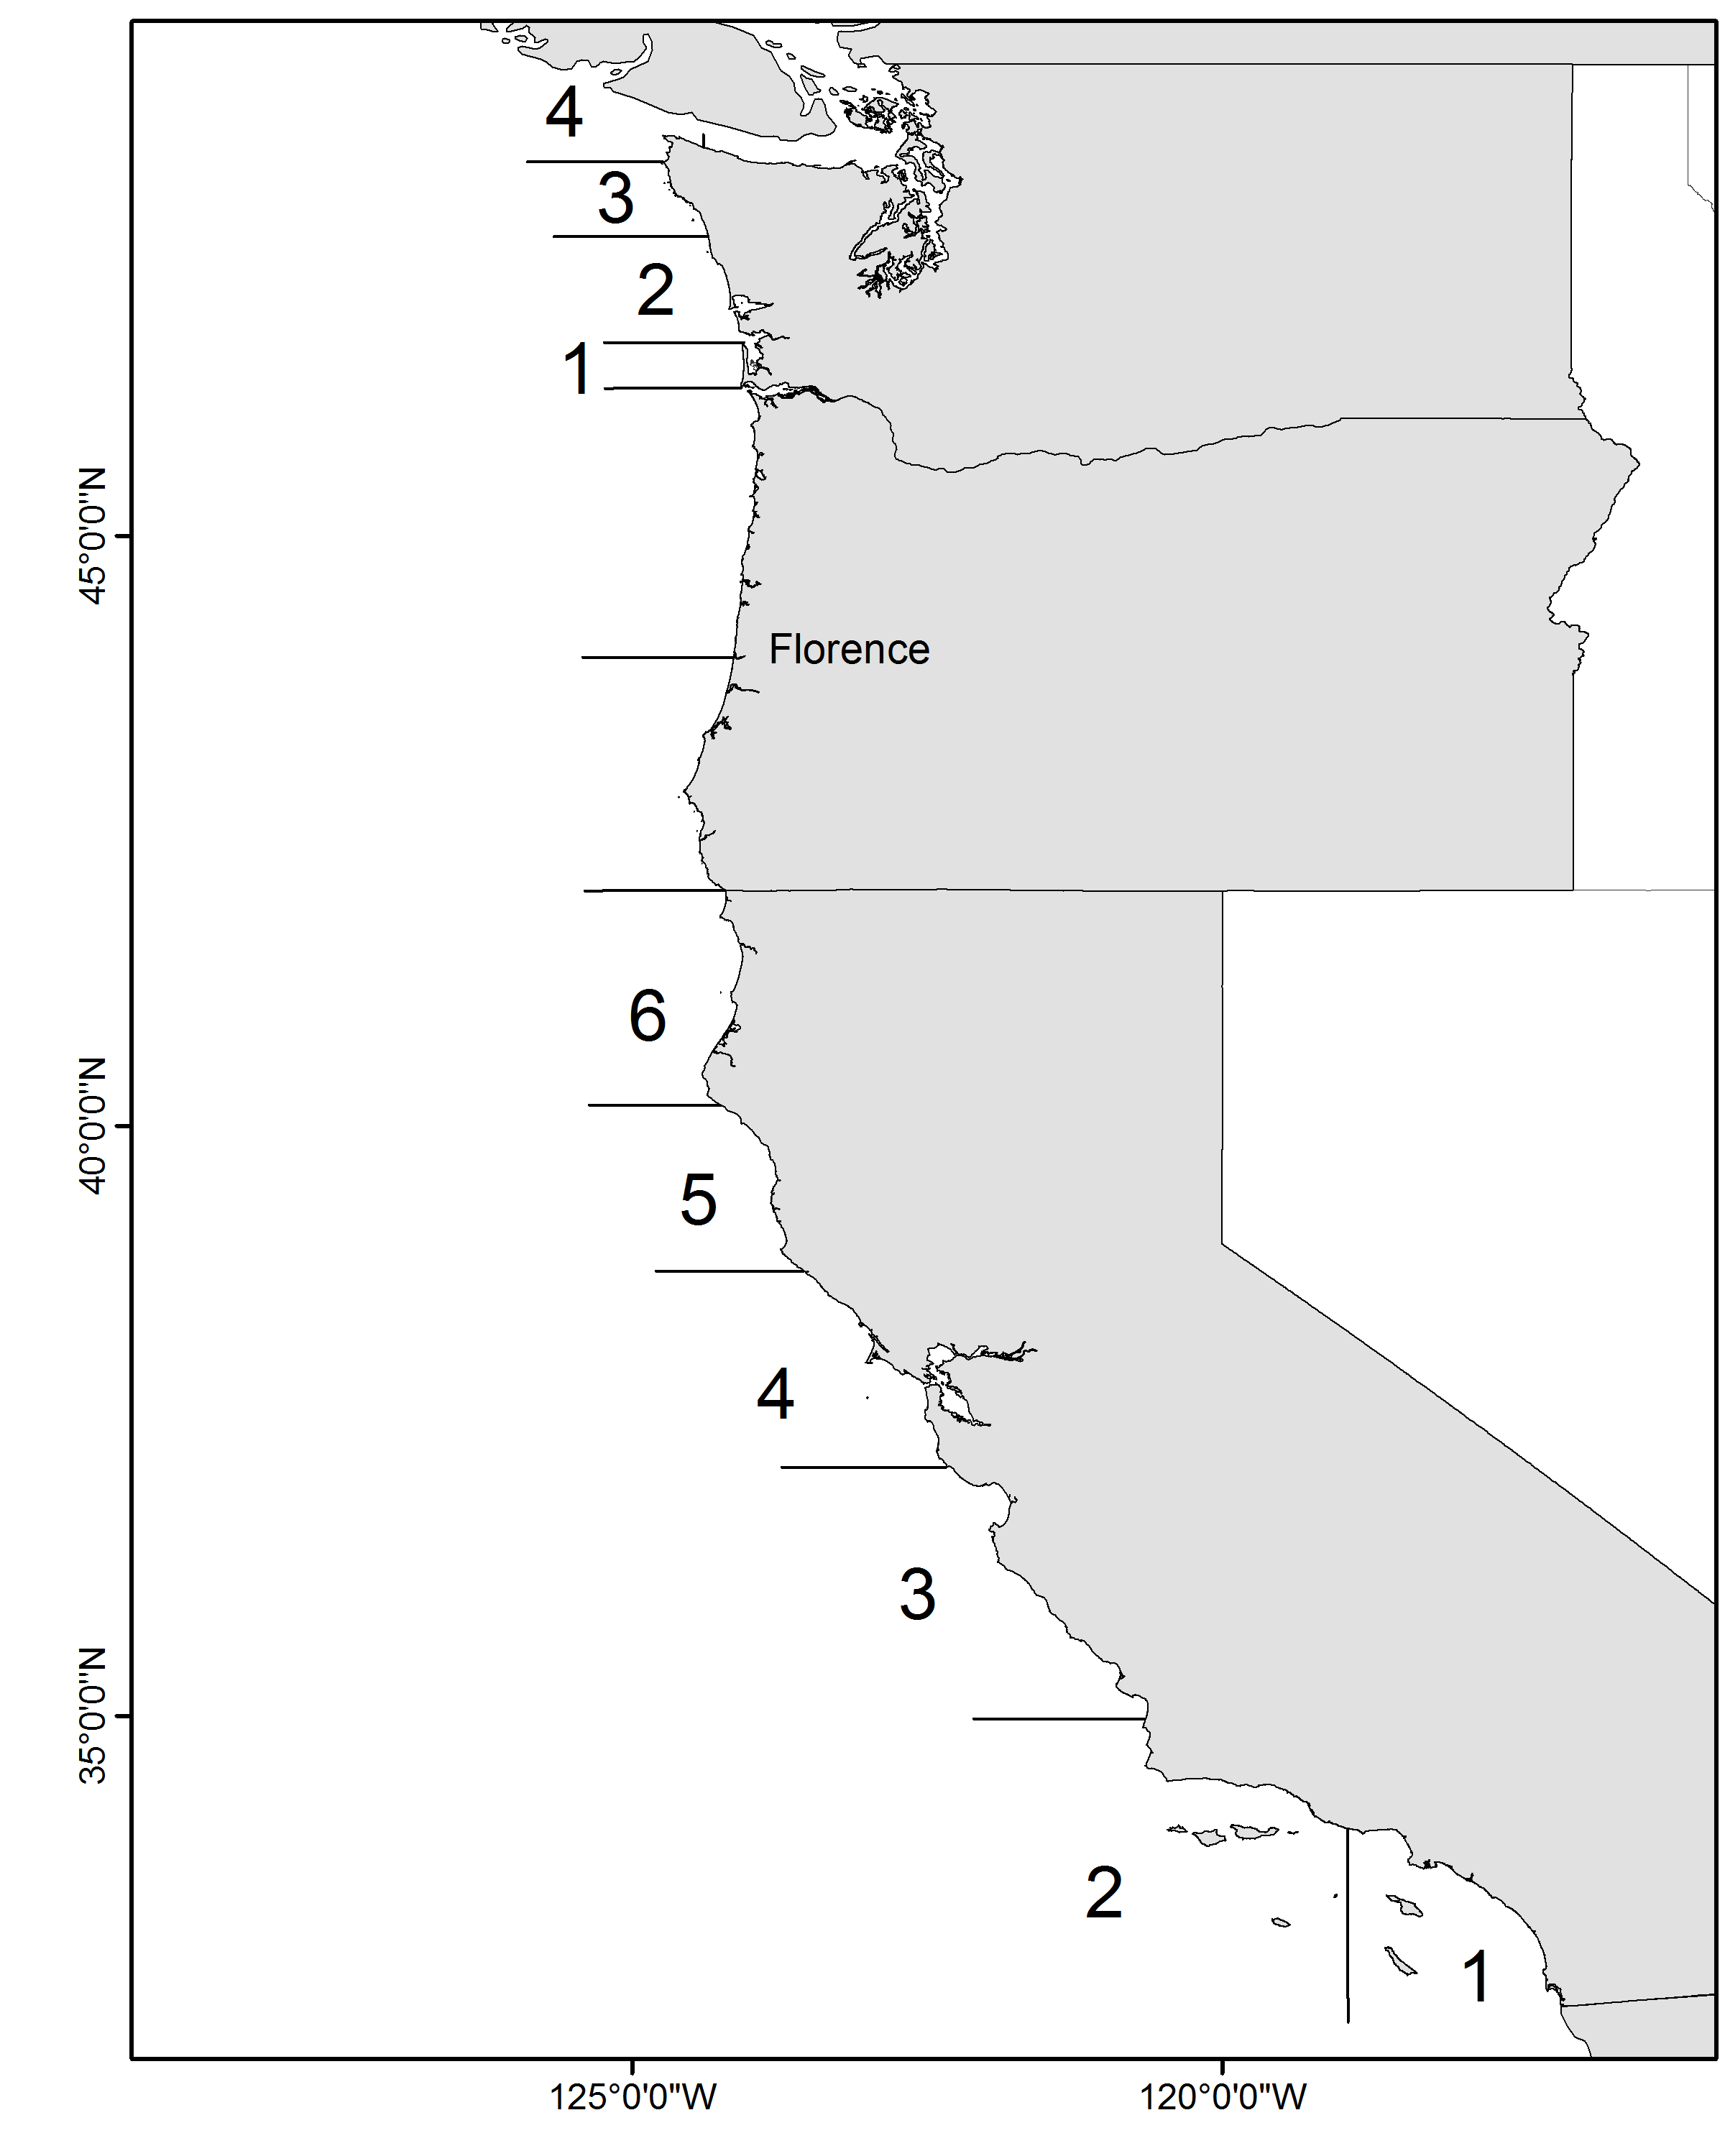
\includegraphics{Figures/boundary_map.png}
\caption{Map showing the state boundary lines for management of the
recreational fishing fleets \label{fig:boundary_map}}
\end{figure}

\begin{figure}
\centering
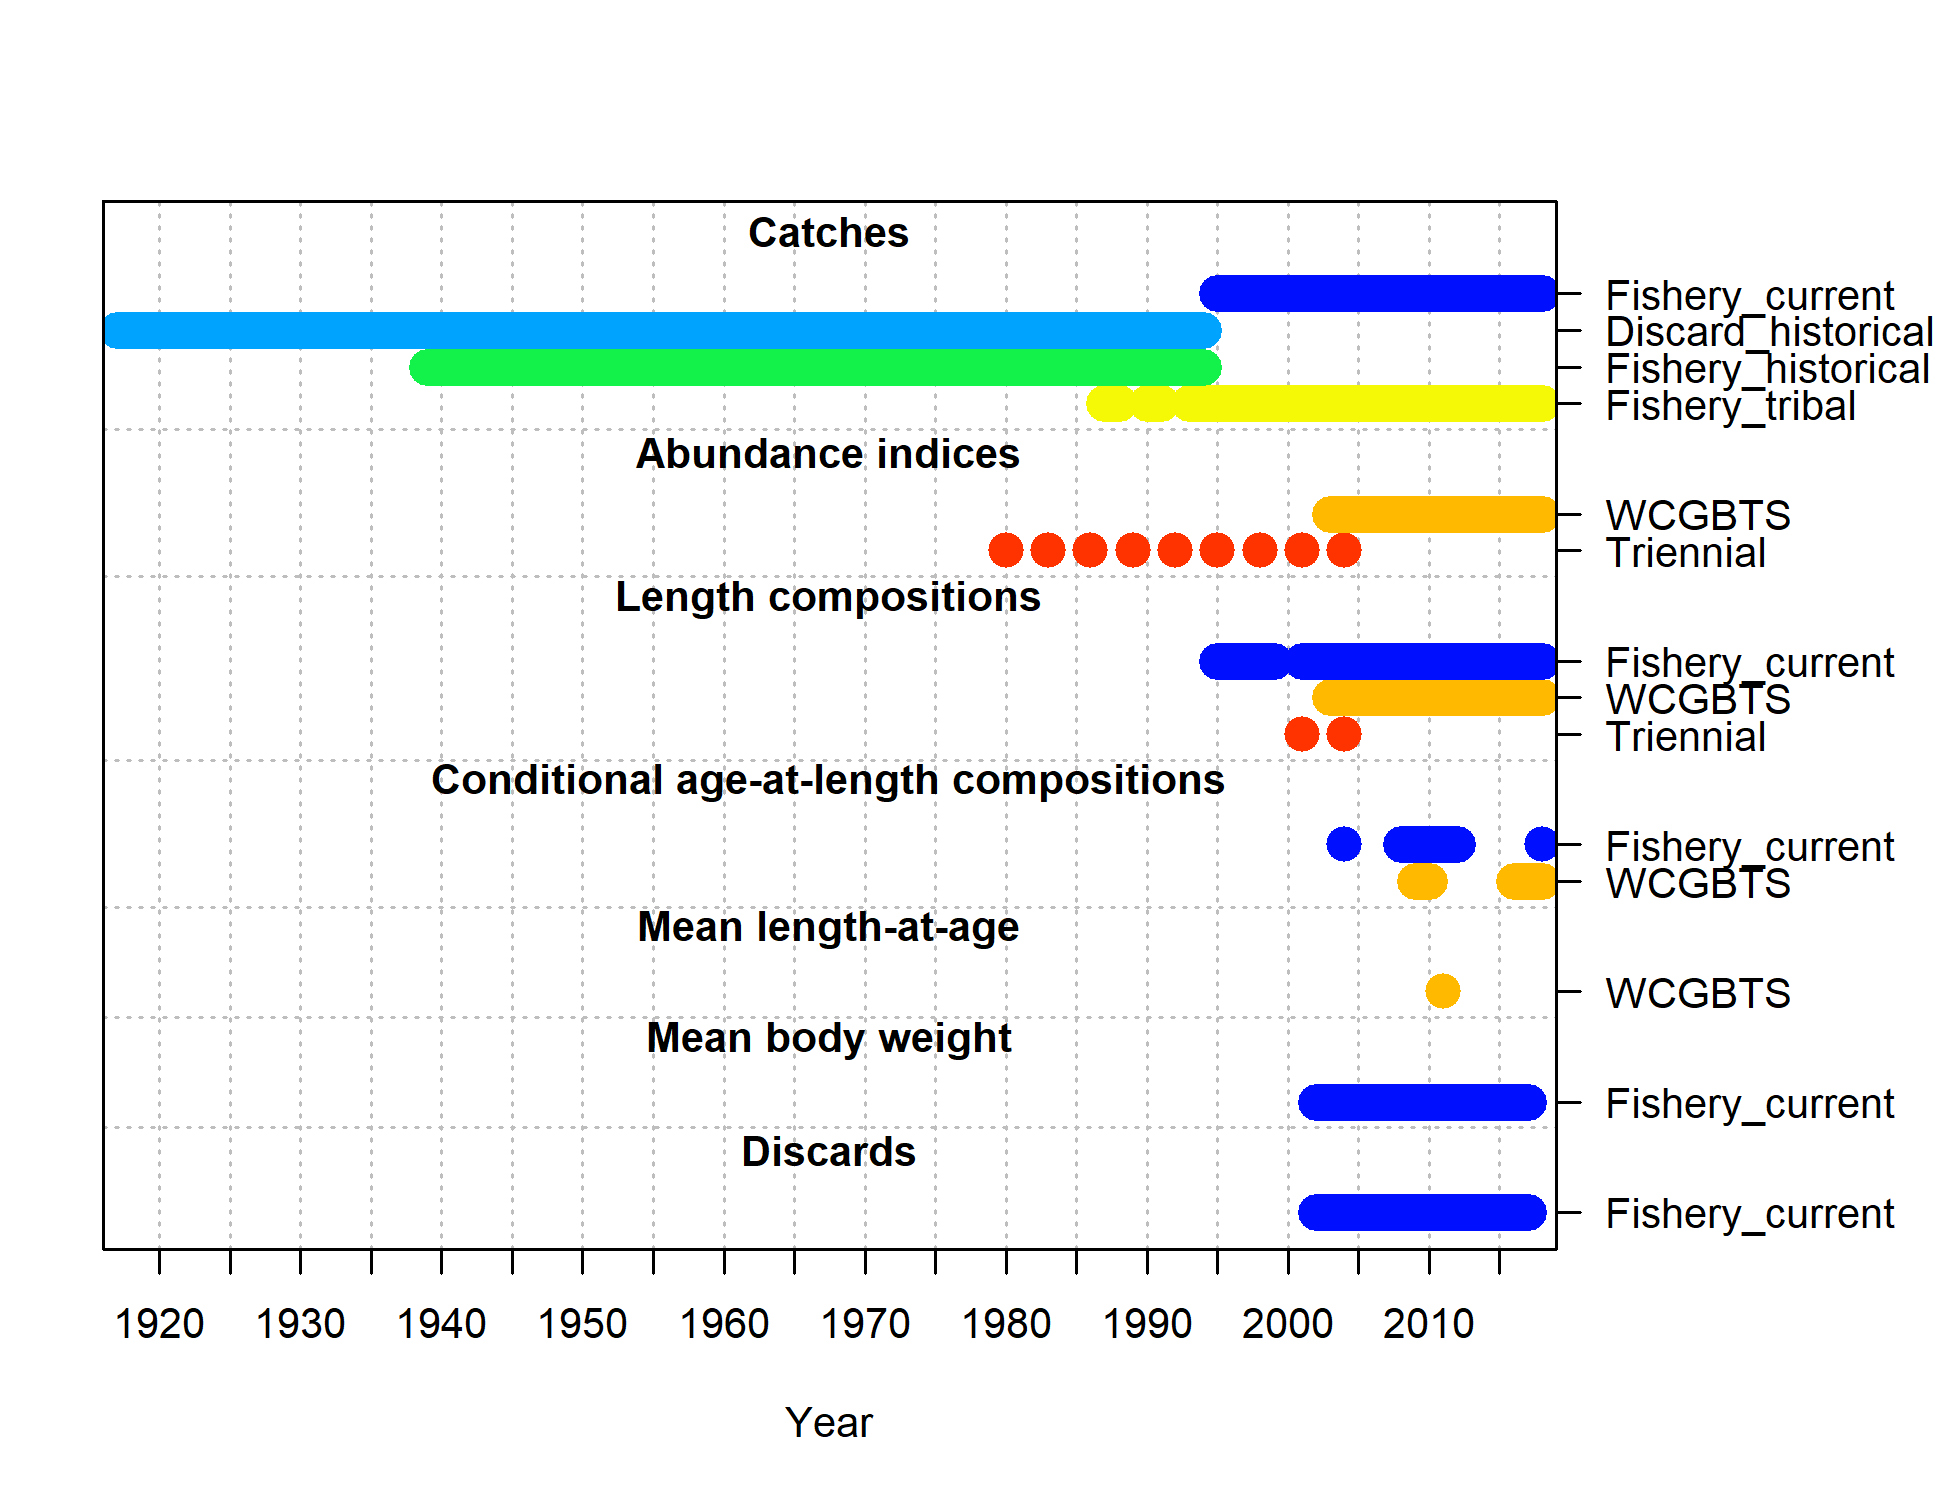
\includegraphics{r4ss/plots_mod1/data_plot.png}
\caption{Summary of data sources used in the model.
\label{fig:data_plot}}
\end{figure}

\FloatBarrier

\FloatBarrier

\FloatBarrier

\FloatBarrier

\FloatBarrier

\FloatBarrier

\FloatBarrier

\newpage

\begin{figure}
\centering
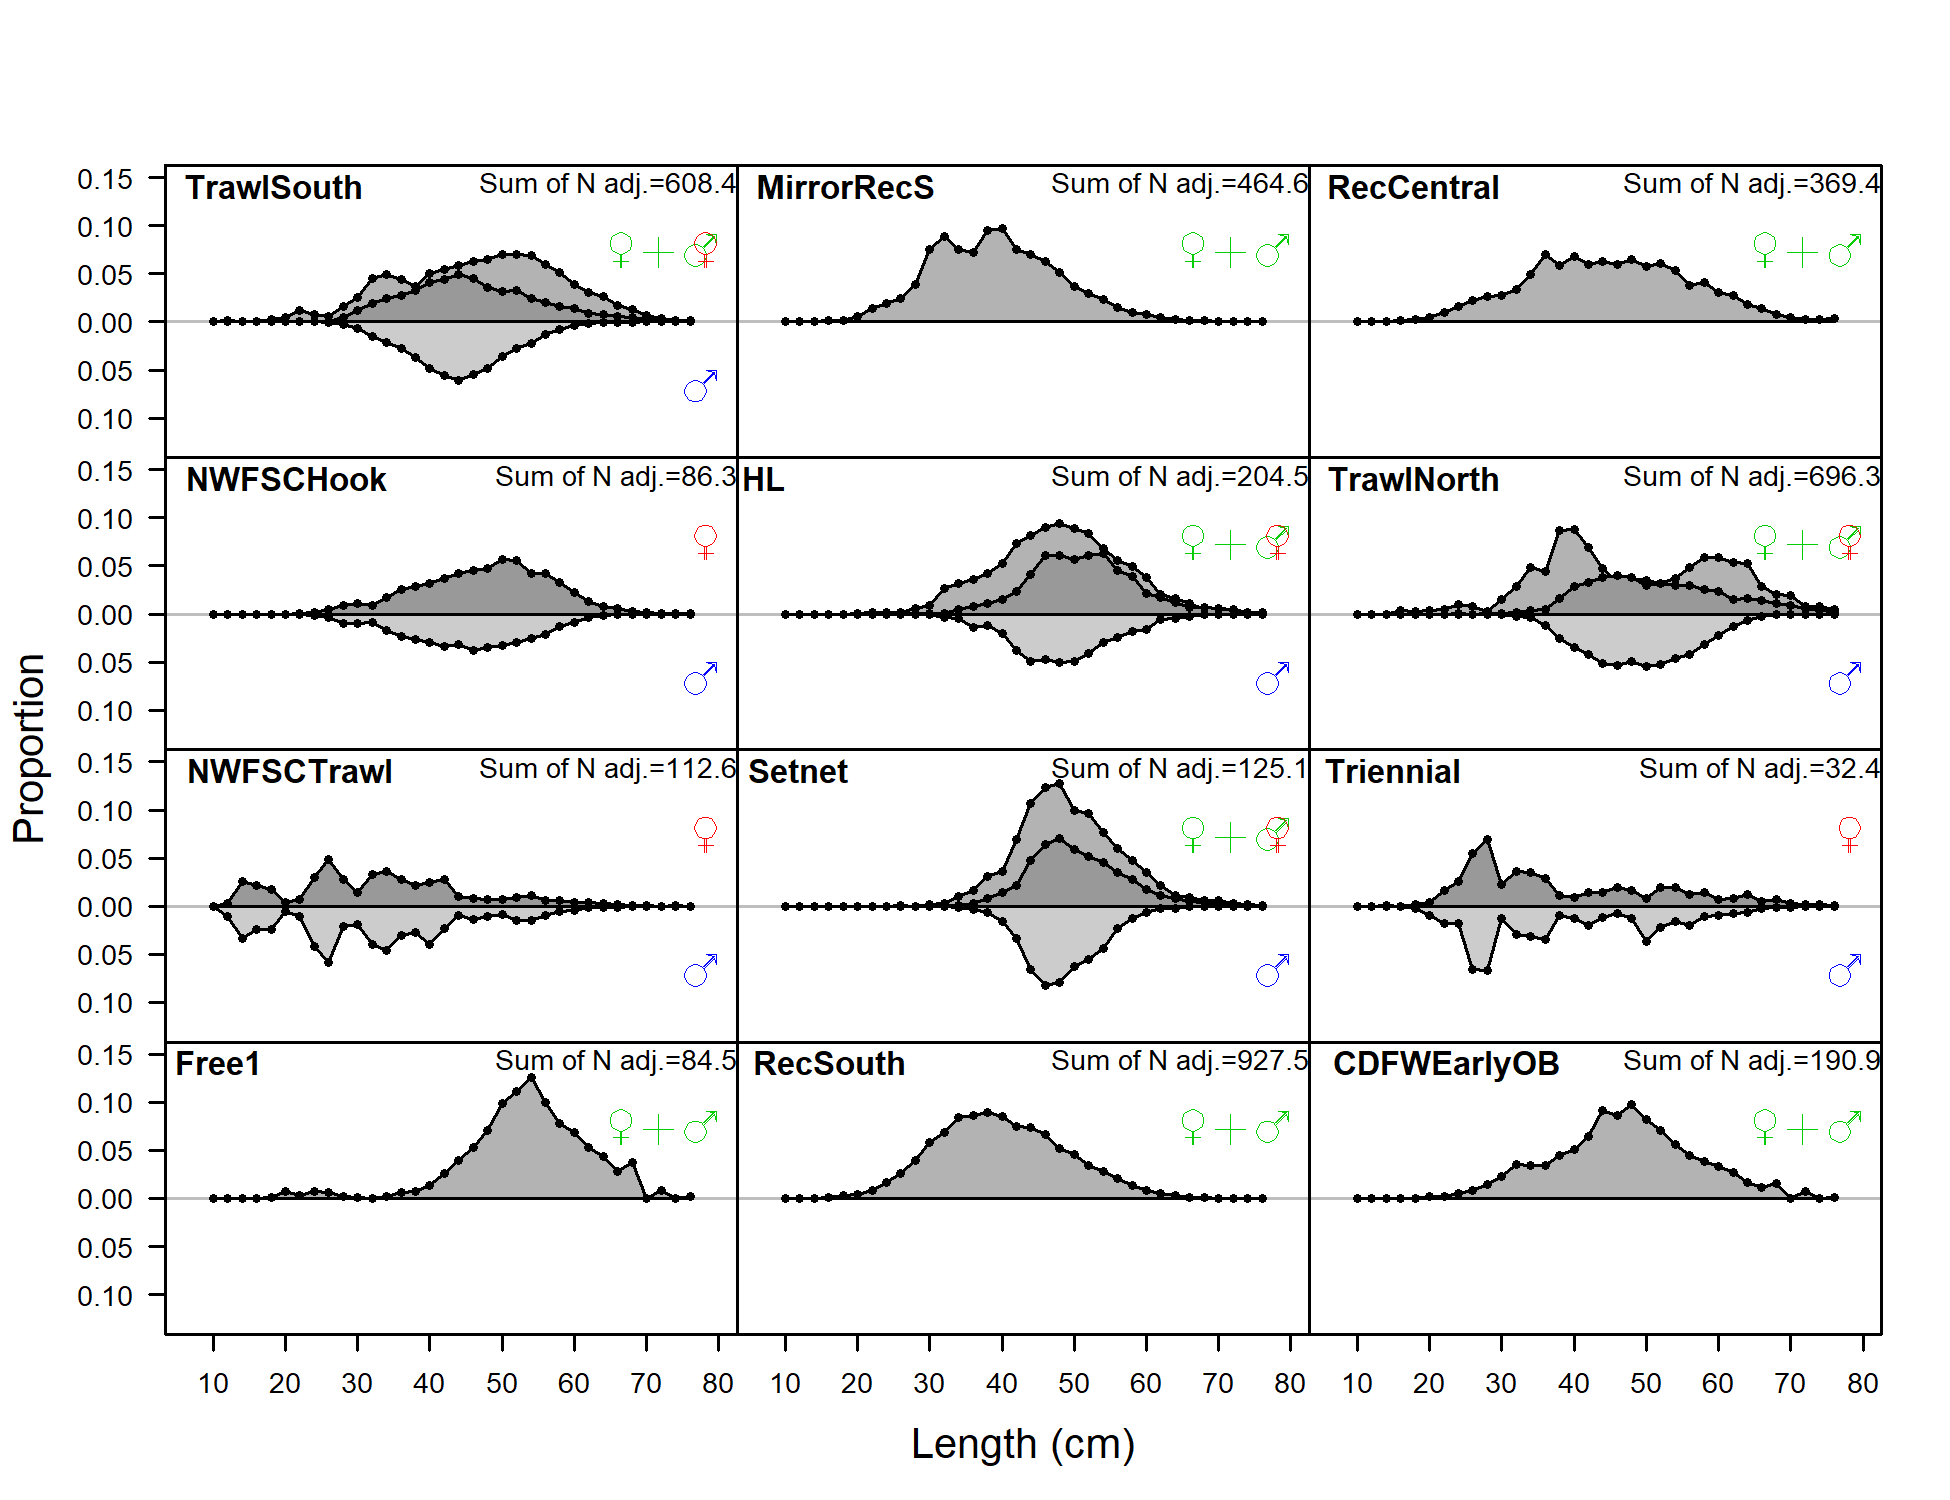
\includegraphics{r4ss/plots_mod1/comp_lendat__aggregated_across_time.png}
\caption{Length comp data, aggregated across time by fleet. Labels
`retained' and `discard' indicate discarded or retained sampled for each
fleet. Panels without this designation represent the whole catch.
\label{fig:comp_lendat_aggregated_across_time}}
\end{figure}

\begin{figure}
\centering
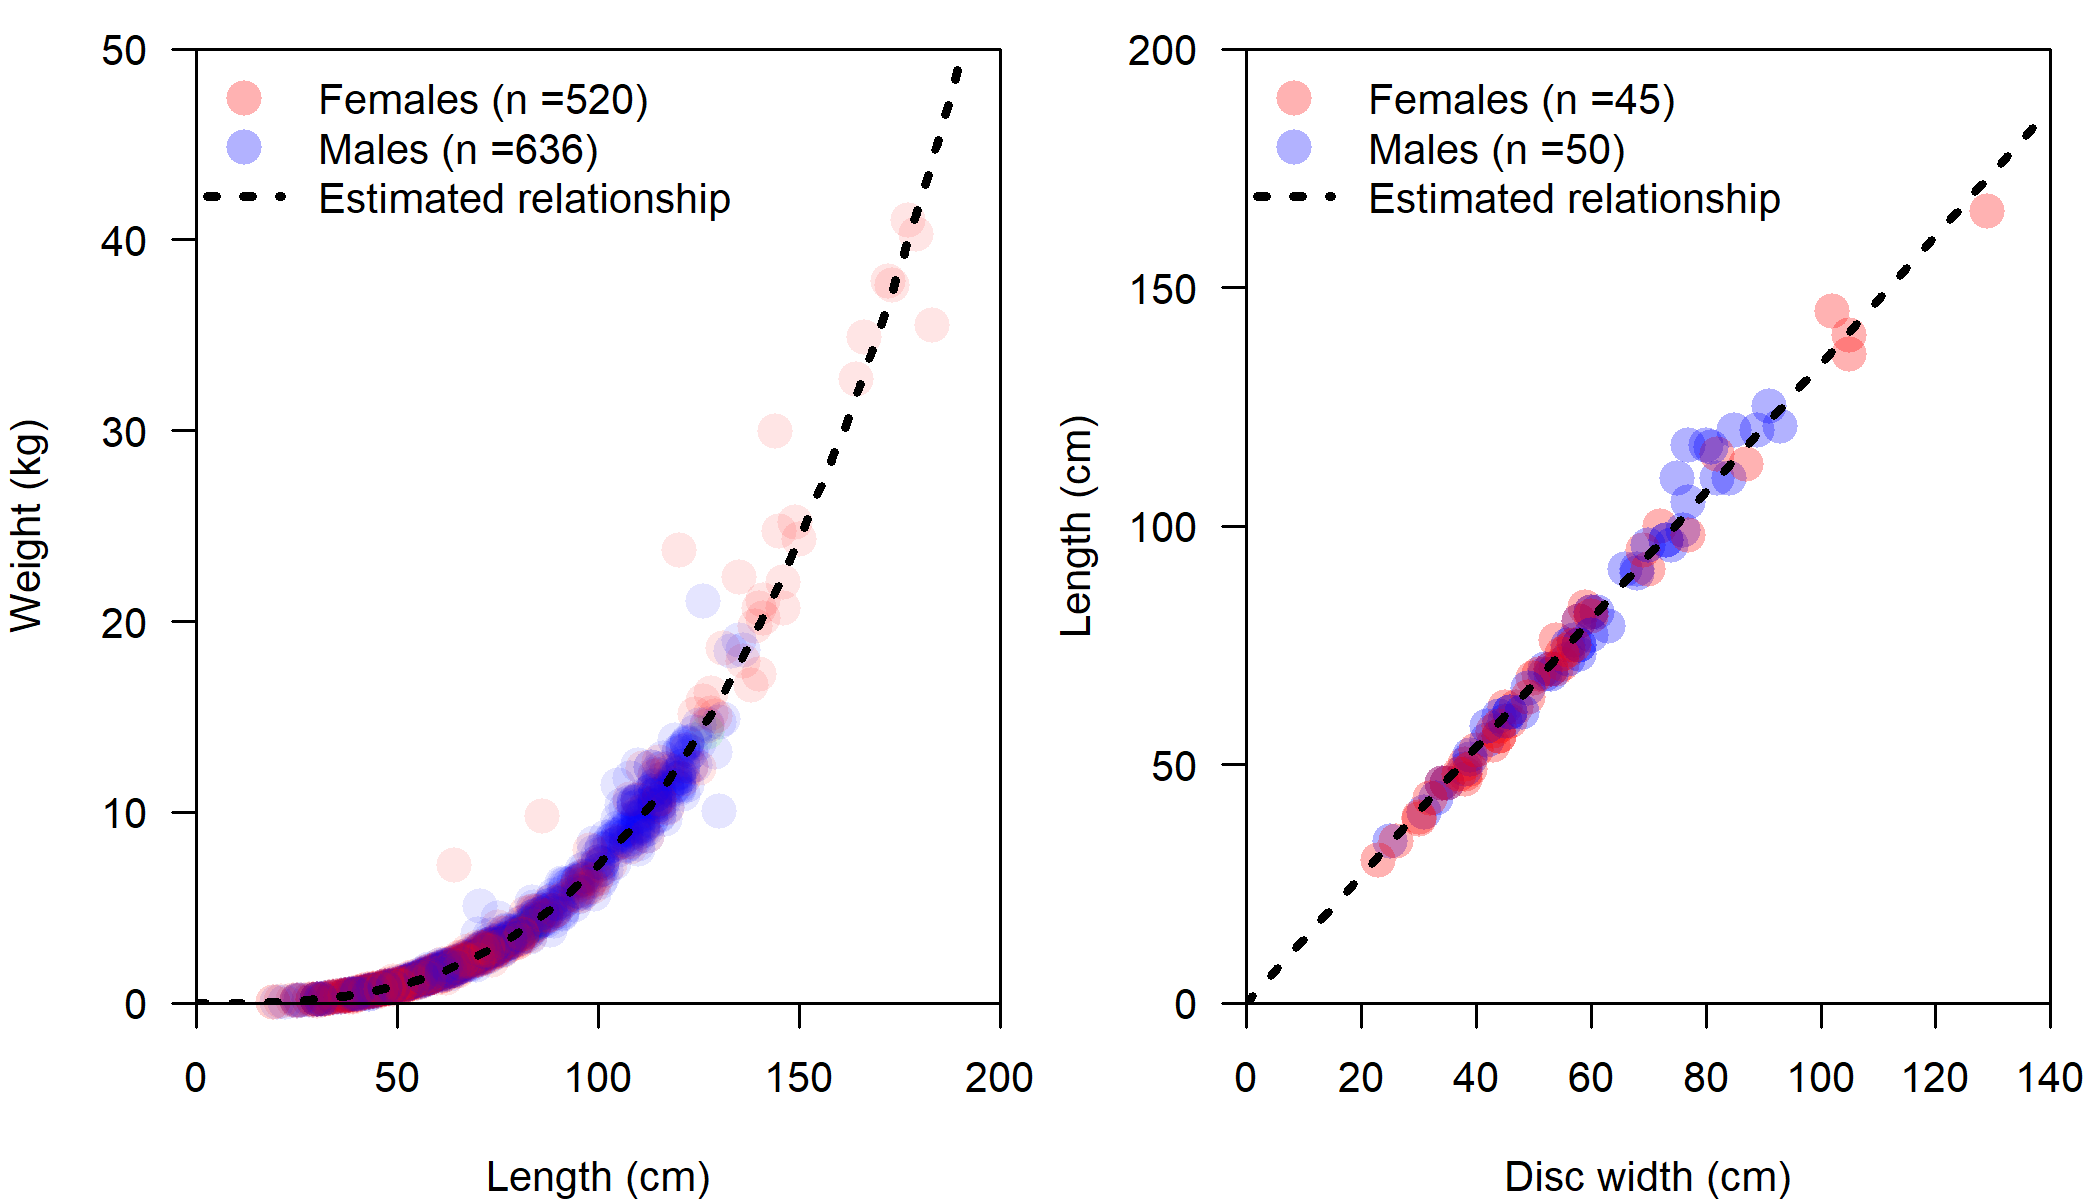
\includegraphics{Figures/Big Skate bio relationships.png}
\caption{Estimated relationship between length and weight (left) and
disc-width and length (right) for Big Skate. Colored points show
observed values and the black line indicates the estimated relationship
\(W = 0.0000074924L^{2.9925}\).\label{fig:weight-length}}
\end{figure}

\begin{figure}
\centering
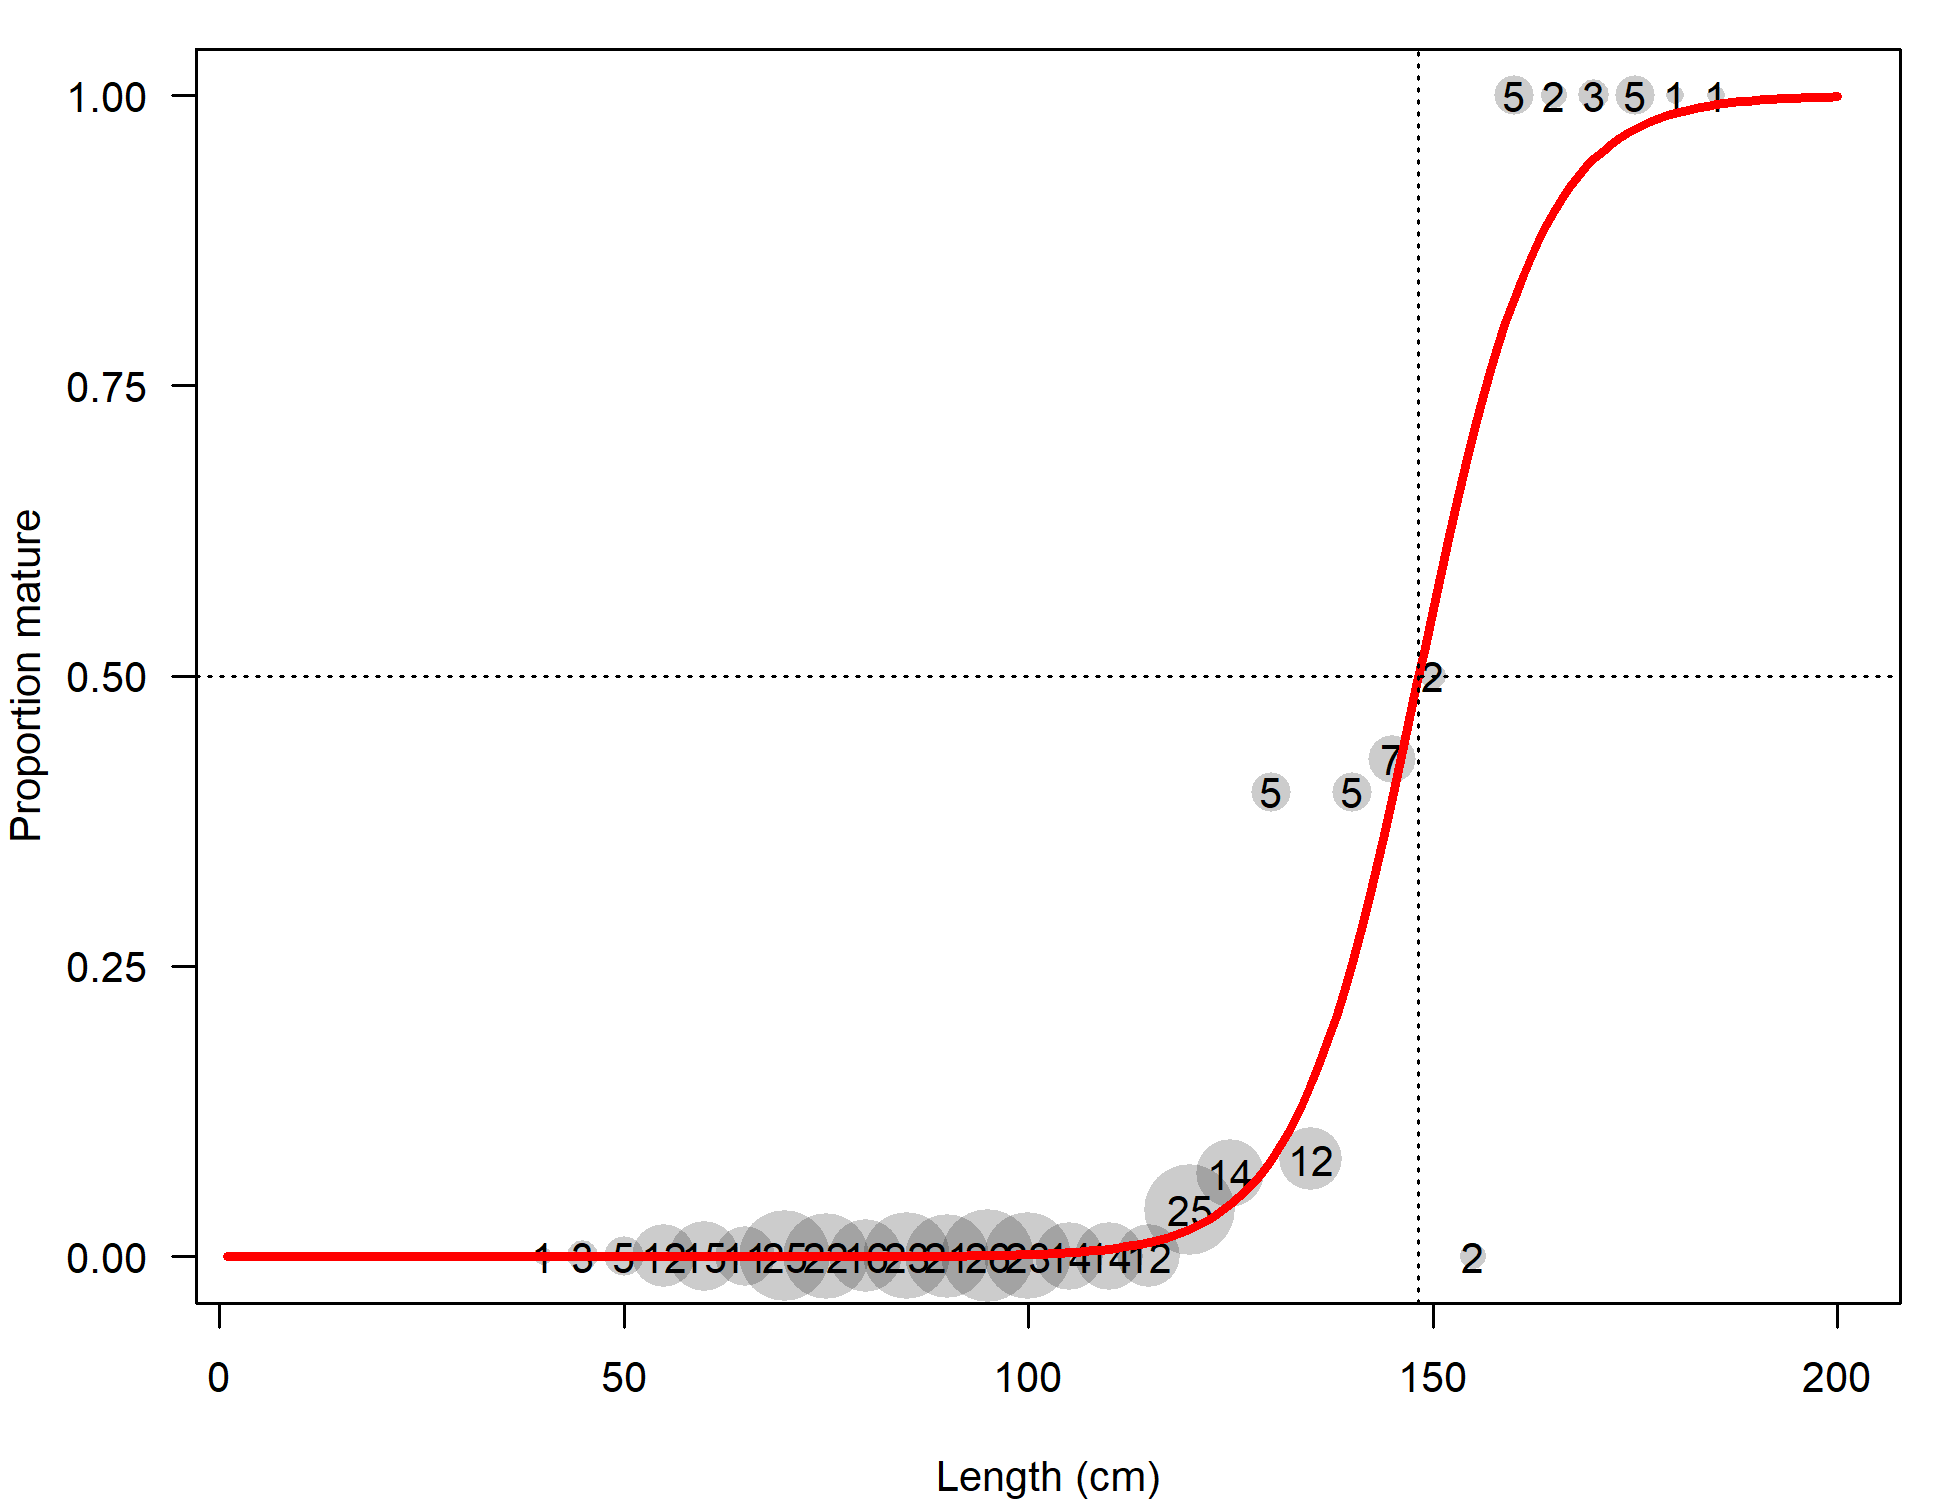
\includegraphics{Figures/BigSkate_maturity.png}
\caption{Estimated maturity relationship for female Big Skate. Gray
points indicate average observed functional maturity within each length
bin with point size proportional to the number of samples (indicated by
text within each point).\label{fig:maturity}}
\end{figure}

\newpage

\FloatBarrier

\FloatBarrier

\FloatBarrier

\FloatBarrier

\begin{figure}
\centering
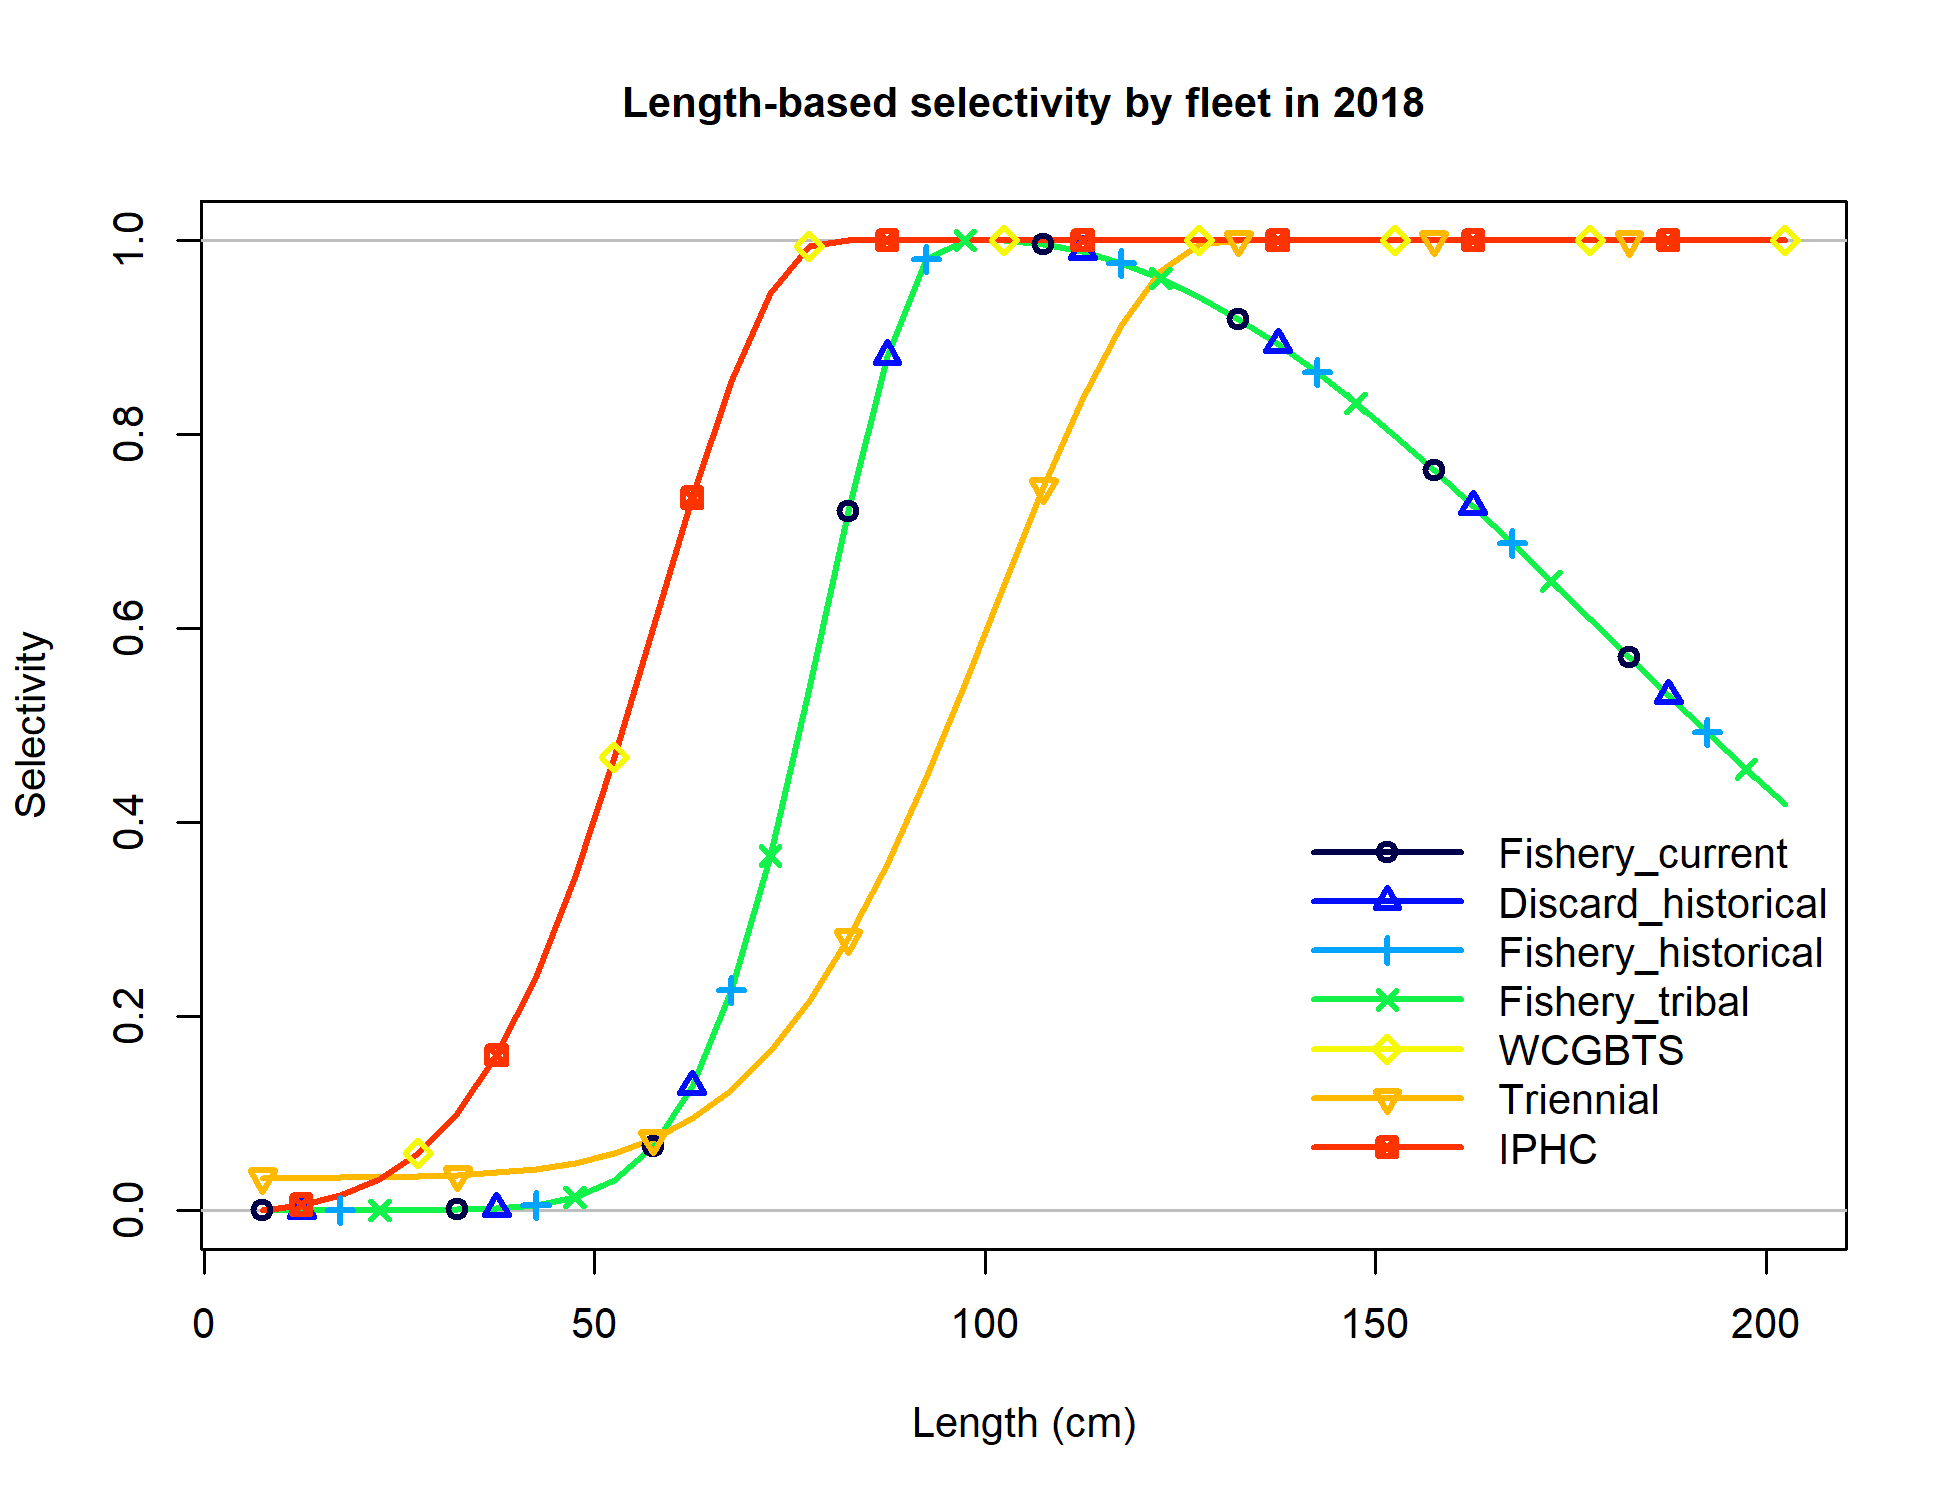
\includegraphics{r4ss/plots_mod1/sel01_multiple_fleets_length1.png}
\caption{Selectivity at length for all of the fleets in the base model.
\label{fig:sel01_multiple_fleets_length1}}
\end{figure}

\FloatBarrier

\begin{figure}
\centering
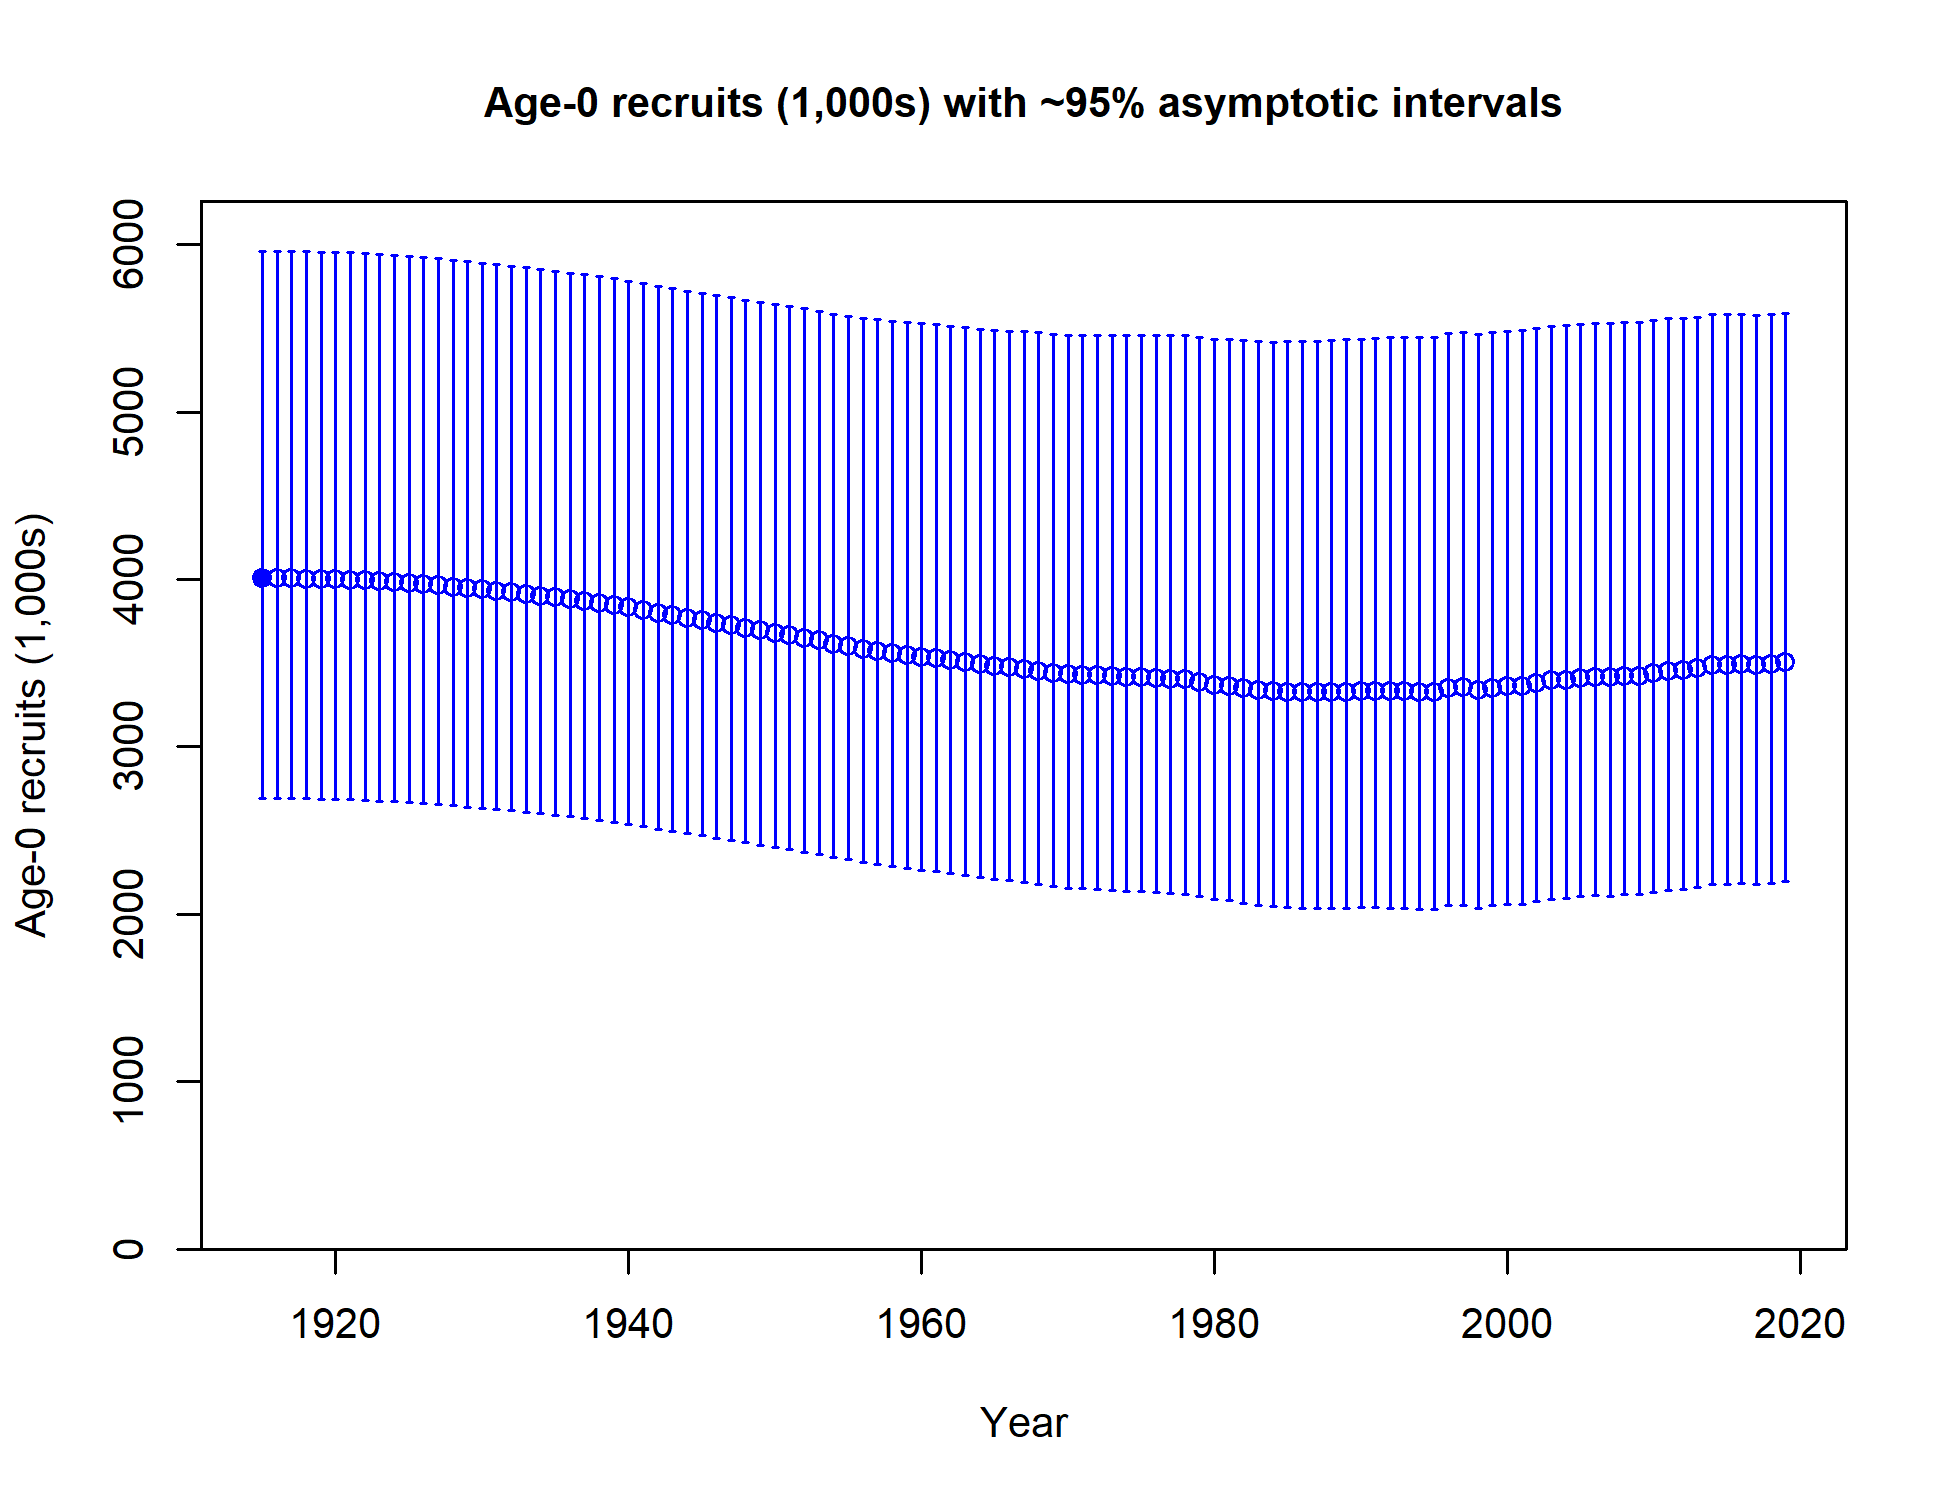
\includegraphics{r4ss/plots_mod1/ts11_Age-0_recruits_(1000s)_with_95_asymptotic_intervals.png}
\caption{Estimated time-series of recruitment for Big Skate.
\label{fig:ts11_Age-0_recruits_(1000s)_with_95_asymptotic_intervals}}
\end{figure}

\begin{figure}
\centering
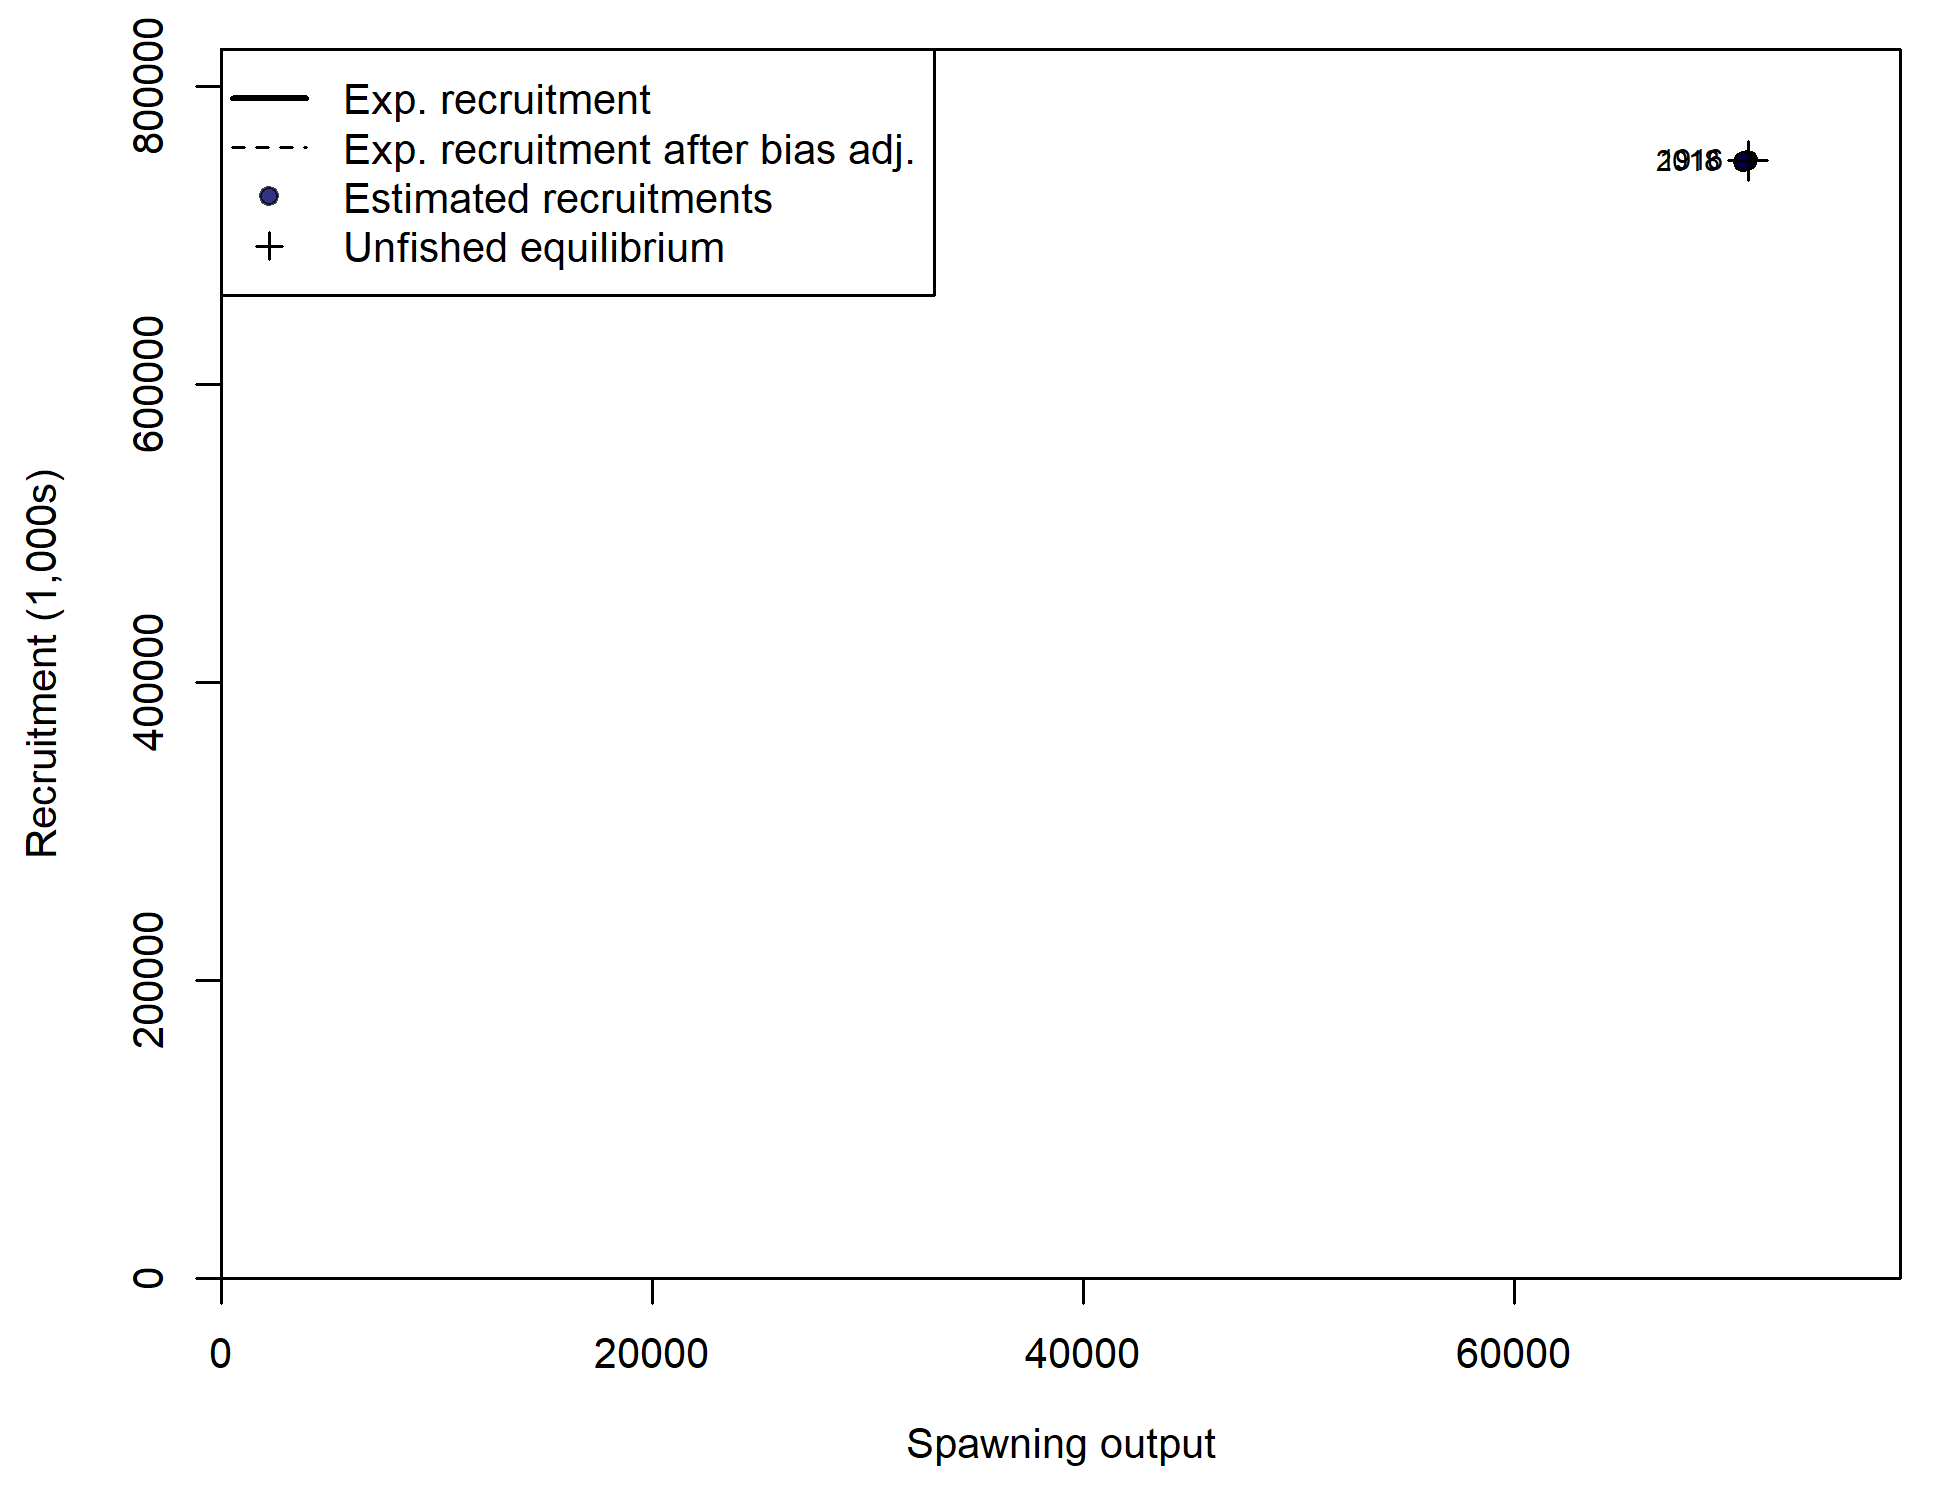
\includegraphics{r4ss/plots_mod1/SR_curve2.png}
\caption{Estimated recruitment (red circles) and the assumed
stock-recruit relationship (black line) for Big Skate. The green line
shows the effect of the bias correction for the lognormal distribution.
\label{fig:SR_curve2}}
\end{figure}

\FloatBarrier

\begin{figure}
\centering
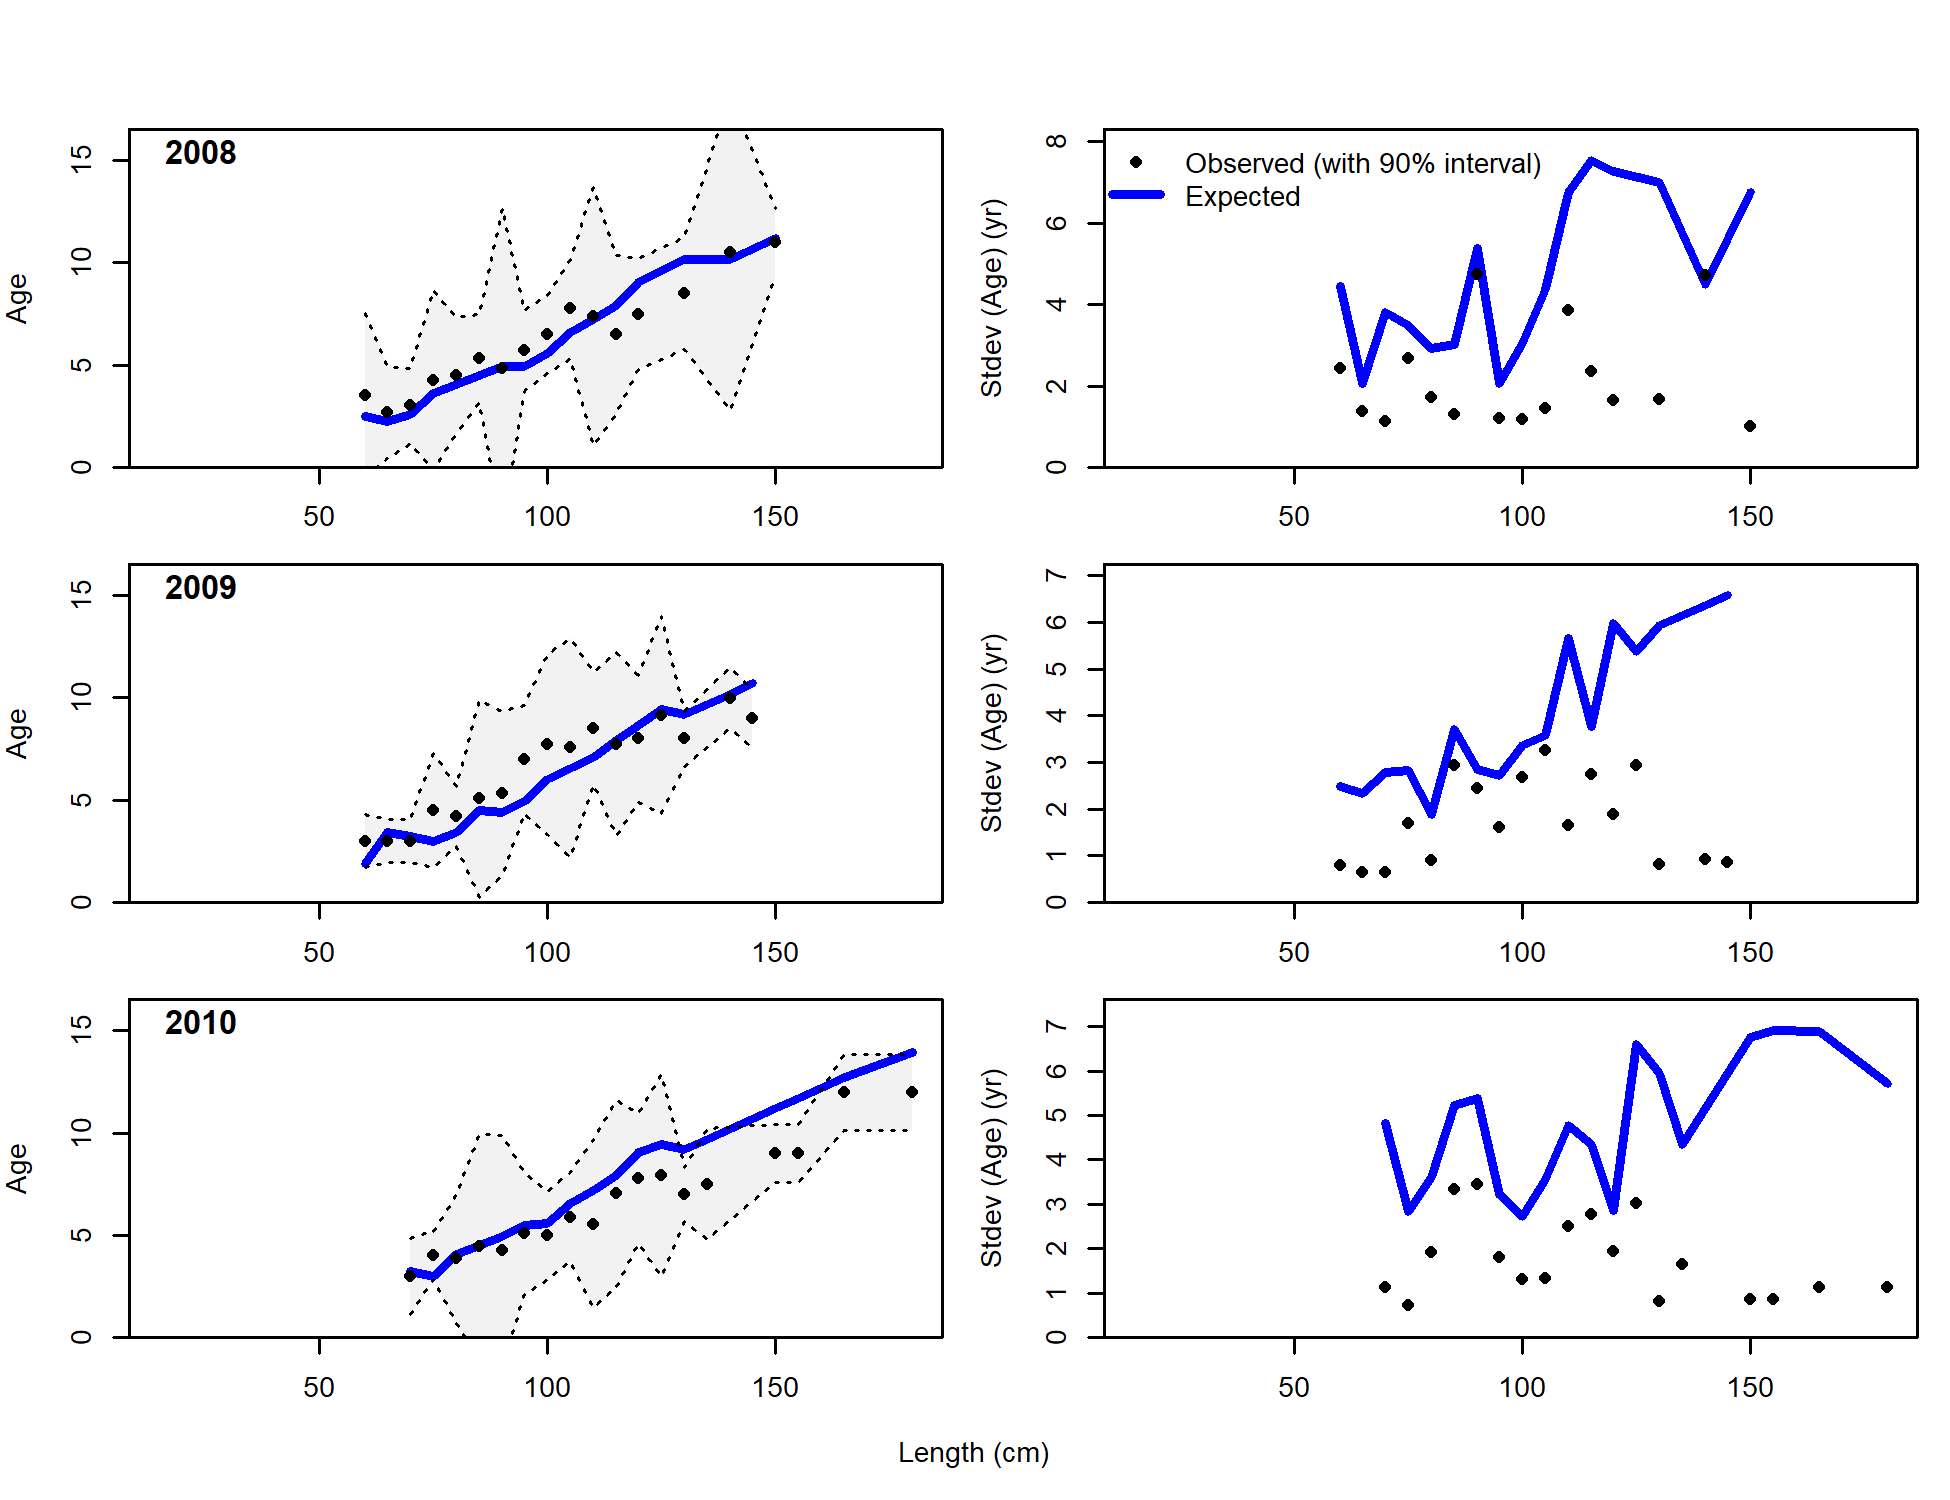
\includegraphics{./r4ss/plots_mod1/comp_condAALfit_Andre_plotsflt1mkt2_page1.png}
\caption{Conditional AAL plot, retained, Fishery (plot 1 of 3) These
plots show mean age and std. dev. in conditional AAL. Left plots are
mean AAL by size\_class (obs. and pred.) with 90\% CIs based on adding
1.64 SE of mean to the data. Right plots in each pair are SE of mean AAL
(obs. and pred.) with 90\% CIs based on the chi\_square distribution.
\label{fig:mod1_4_comp_condAALfit_Andre_plotsflt1mkt2_page1}}
\end{figure}

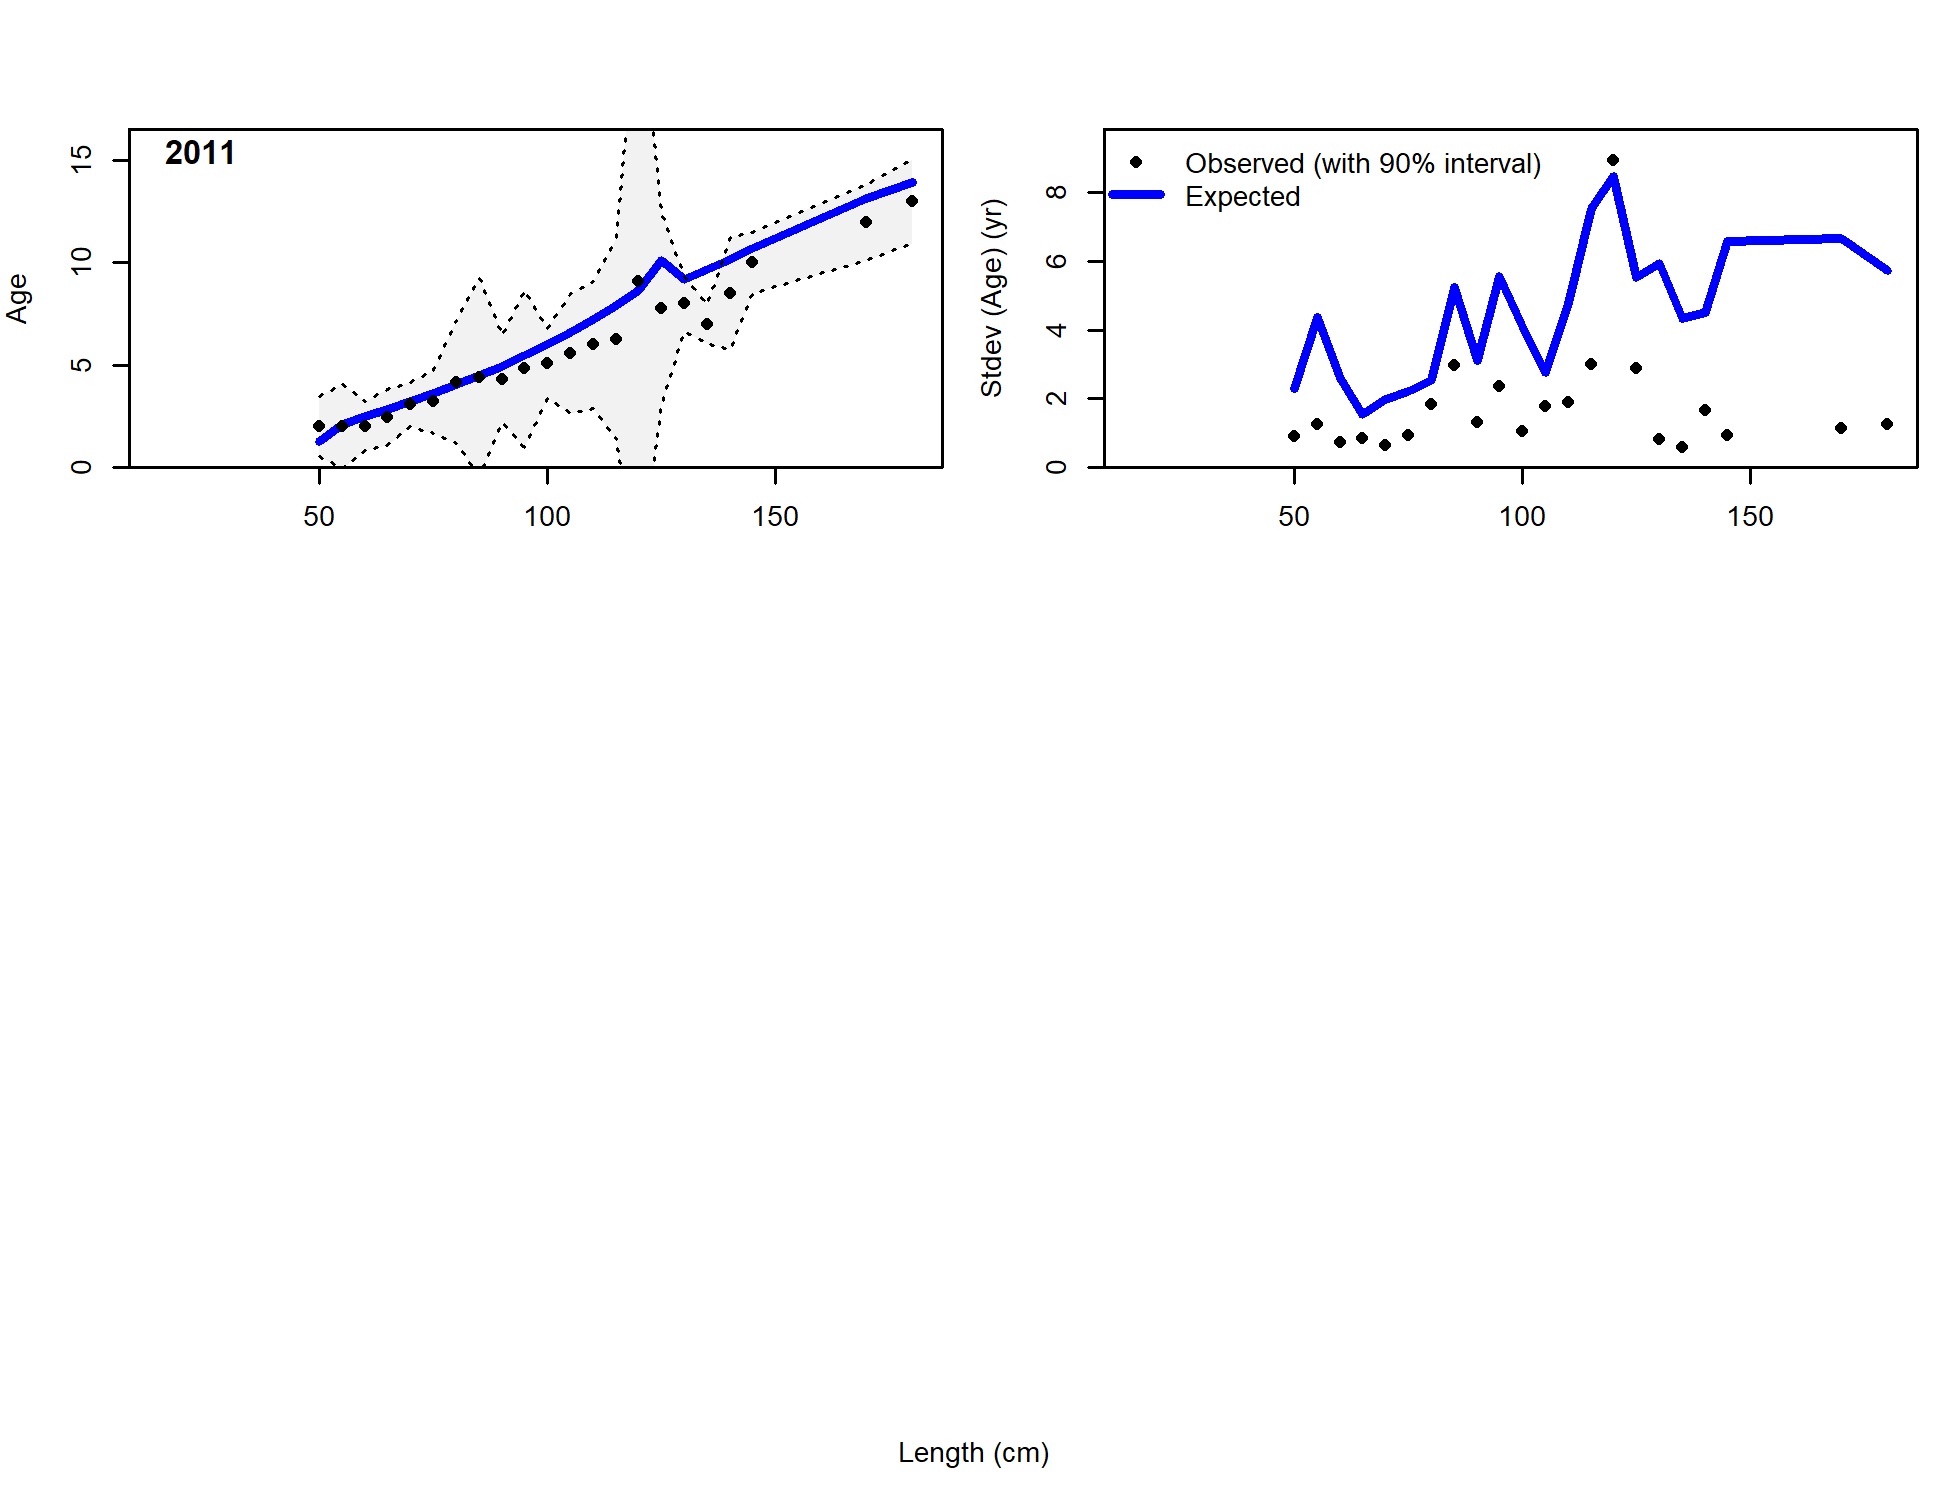
\includegraphics{./r4ss/plots_mod1/comp_condAALfit_Andre_plotsflt1mkt2_page2.png}

\begin{center} 

              Figure continued from previous page 

             \end{center}

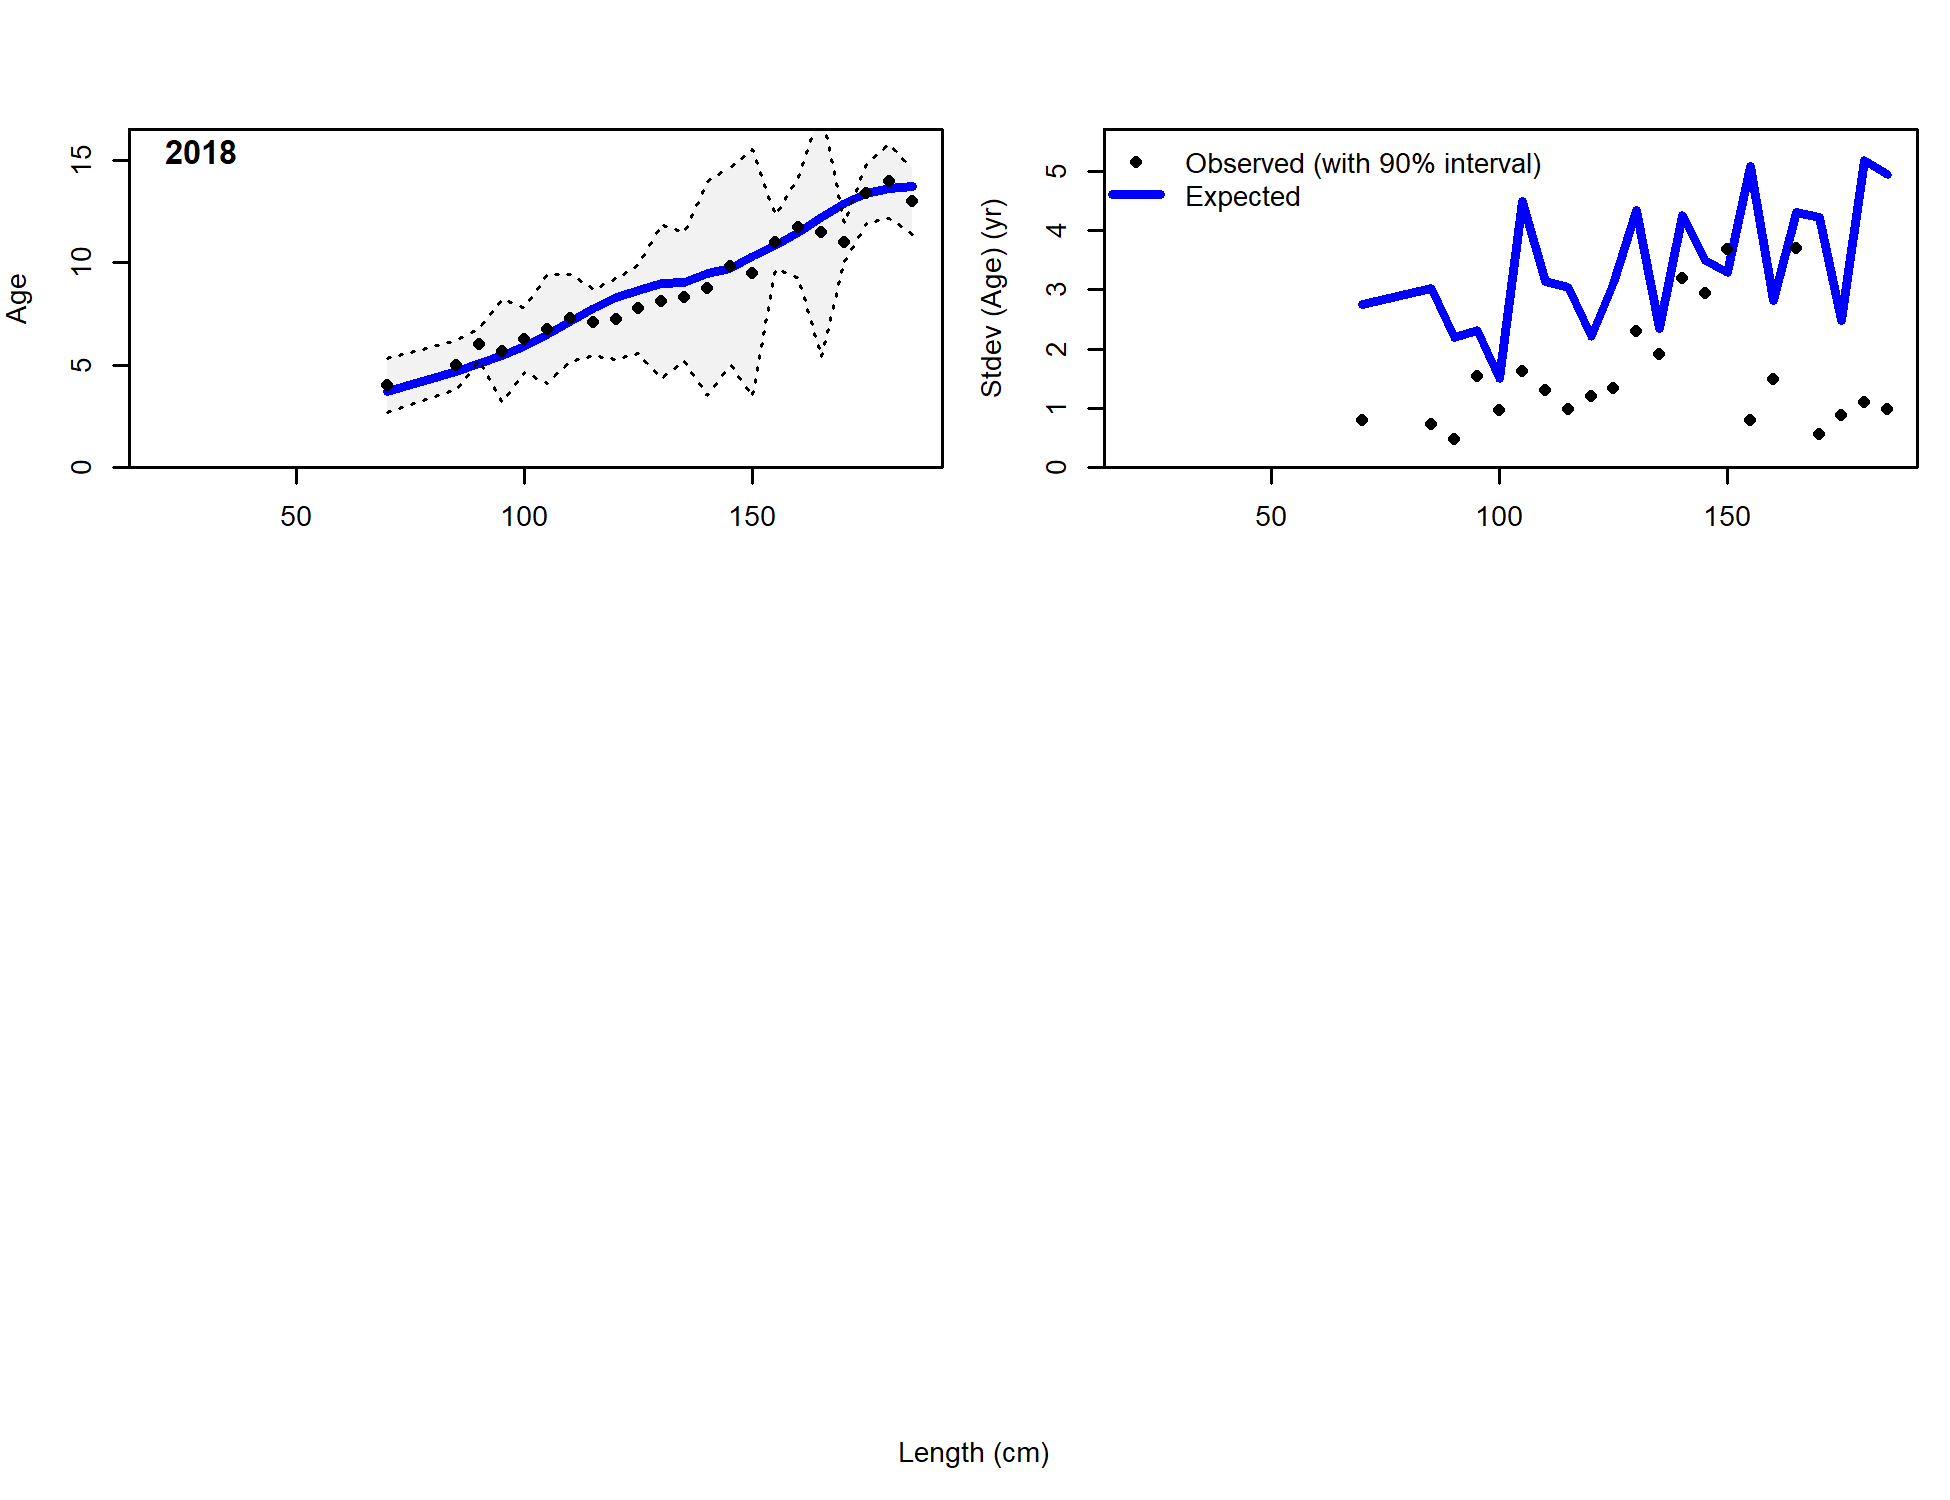
\includegraphics{./r4ss/plots_mod1/comp_condAALfit_Andre_plotsflt1mkt2_page3.png}

\begin{center} 

              Figure continued from previous page 

             \end{center}

\begin{figure}
\centering
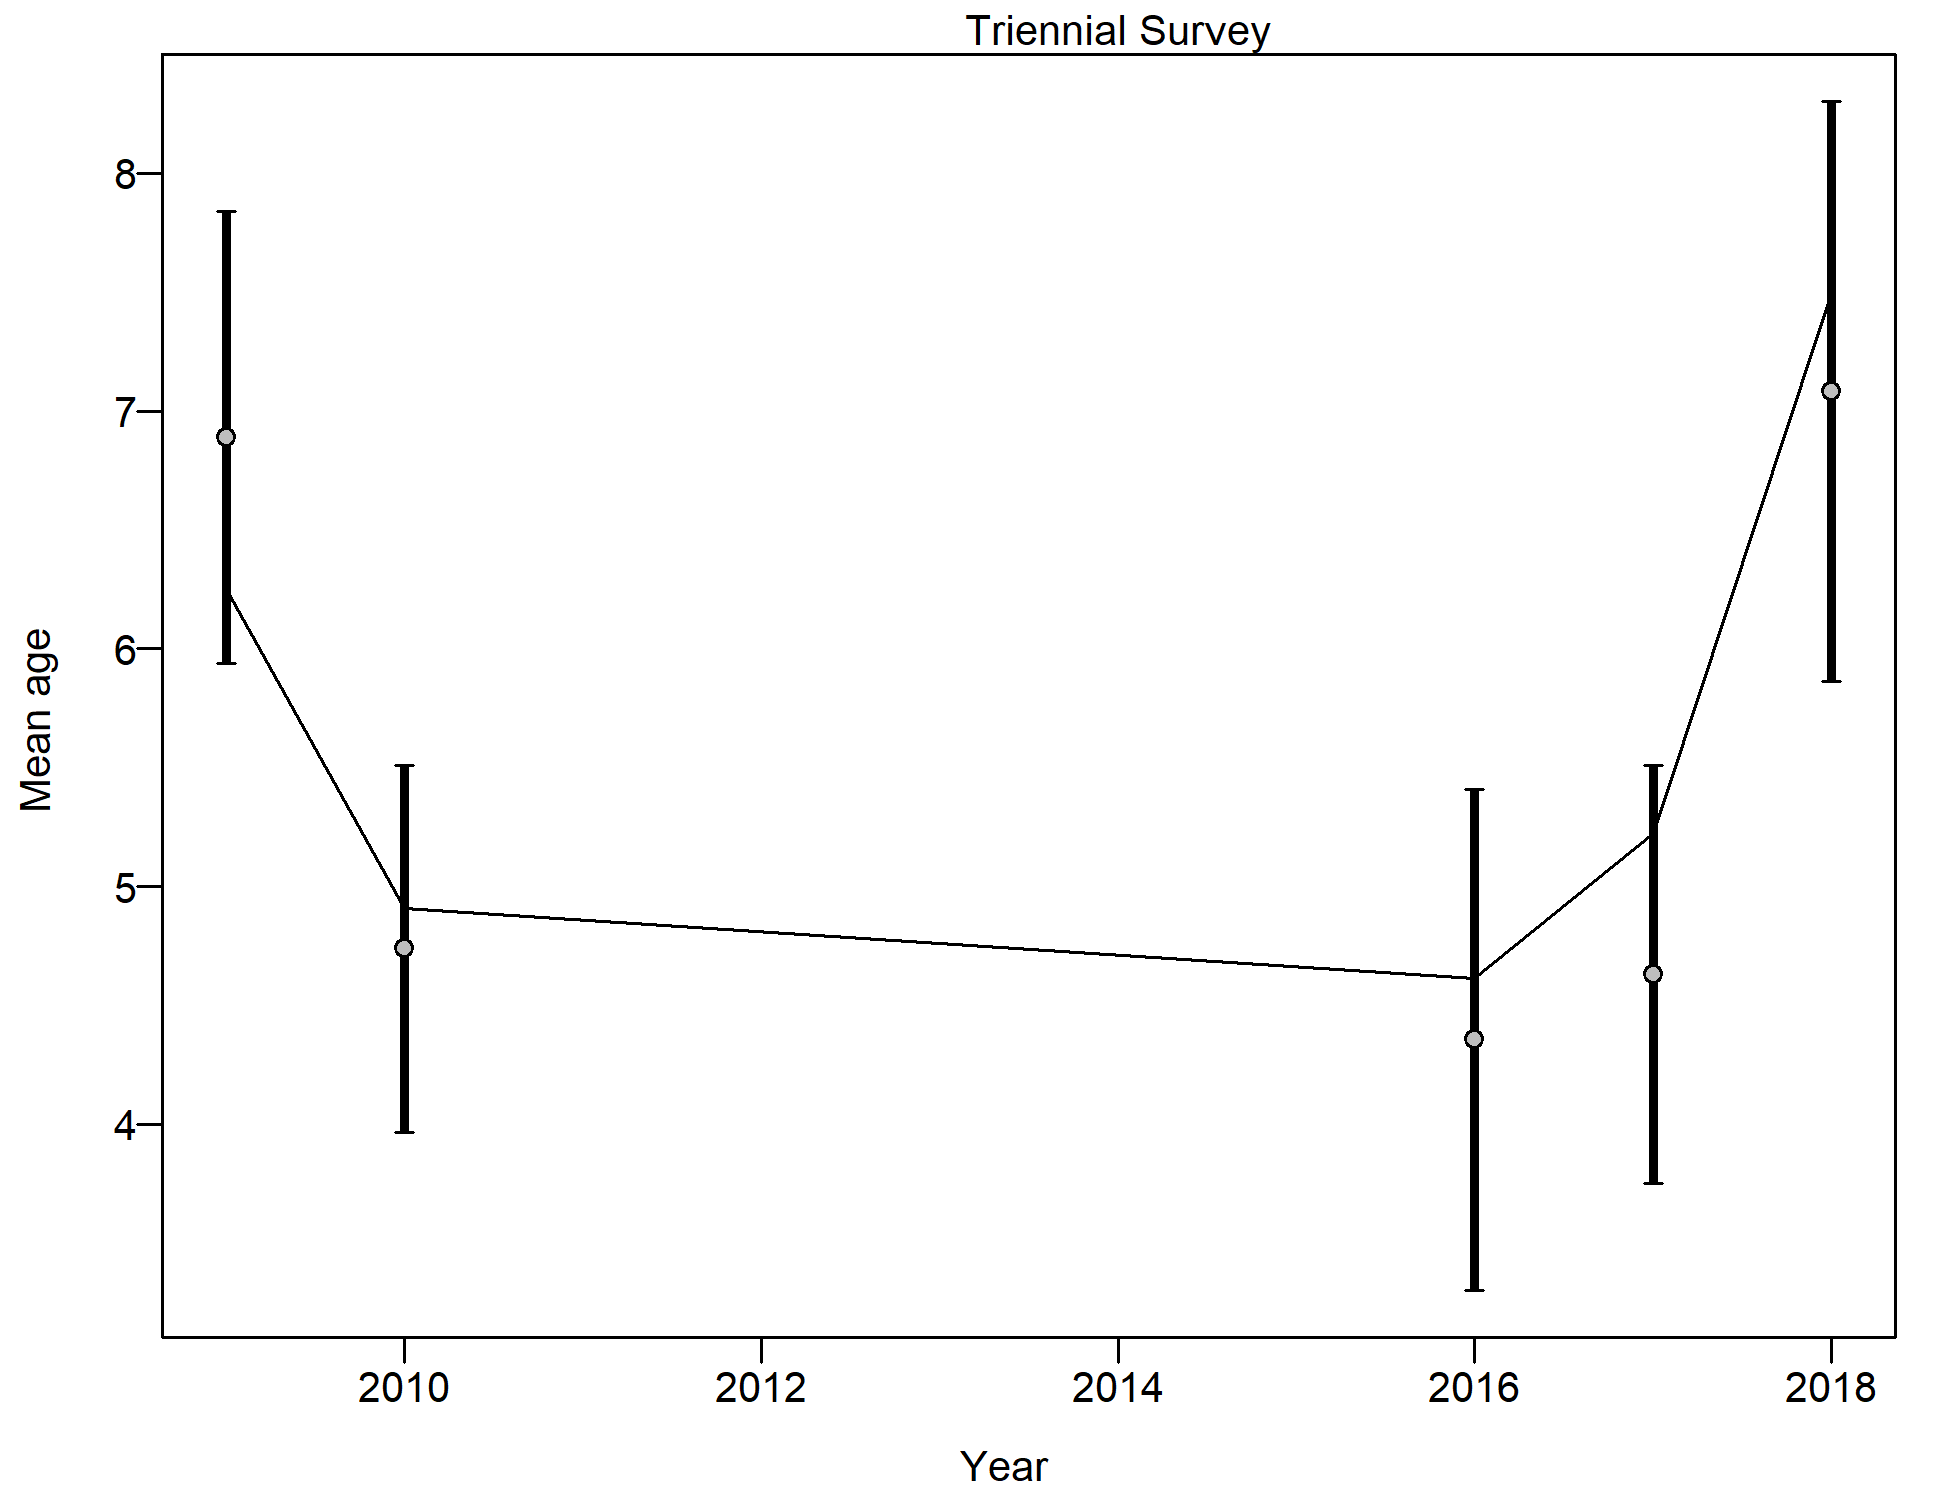
\includegraphics{./r4ss/plots_mod1/comp_condAALfit_data_weighting_TA1.8_condAgeTriennial Survey.png}
\caption{Mean age from conditional data (aggregated across length bins)
for Triennial Survey with 95\% confidence intervals based on current
samples sizes. Francis data weighting method TA1.8: thinner intervals
(with capped ends) show result of further adjusting sample sizes based
on suggested multiplier (with 95\% interval) for conditional
age\_at\_length data from Triennial Survey: 1.0013 (0.5403\_106.6286)
For more info, see Francis, R.I.C.C. (2011). Data weighting in
statistical fisheries stock assessment models. Can. J. Fish. Aquat. Sci.
68: 1124\_1138.
\label{fig:mod1_7_comp_condAALfit_data_weighting_TA1.8_condAgeTriennial Survey}}
\end{figure}

\begin{figure}
\centering
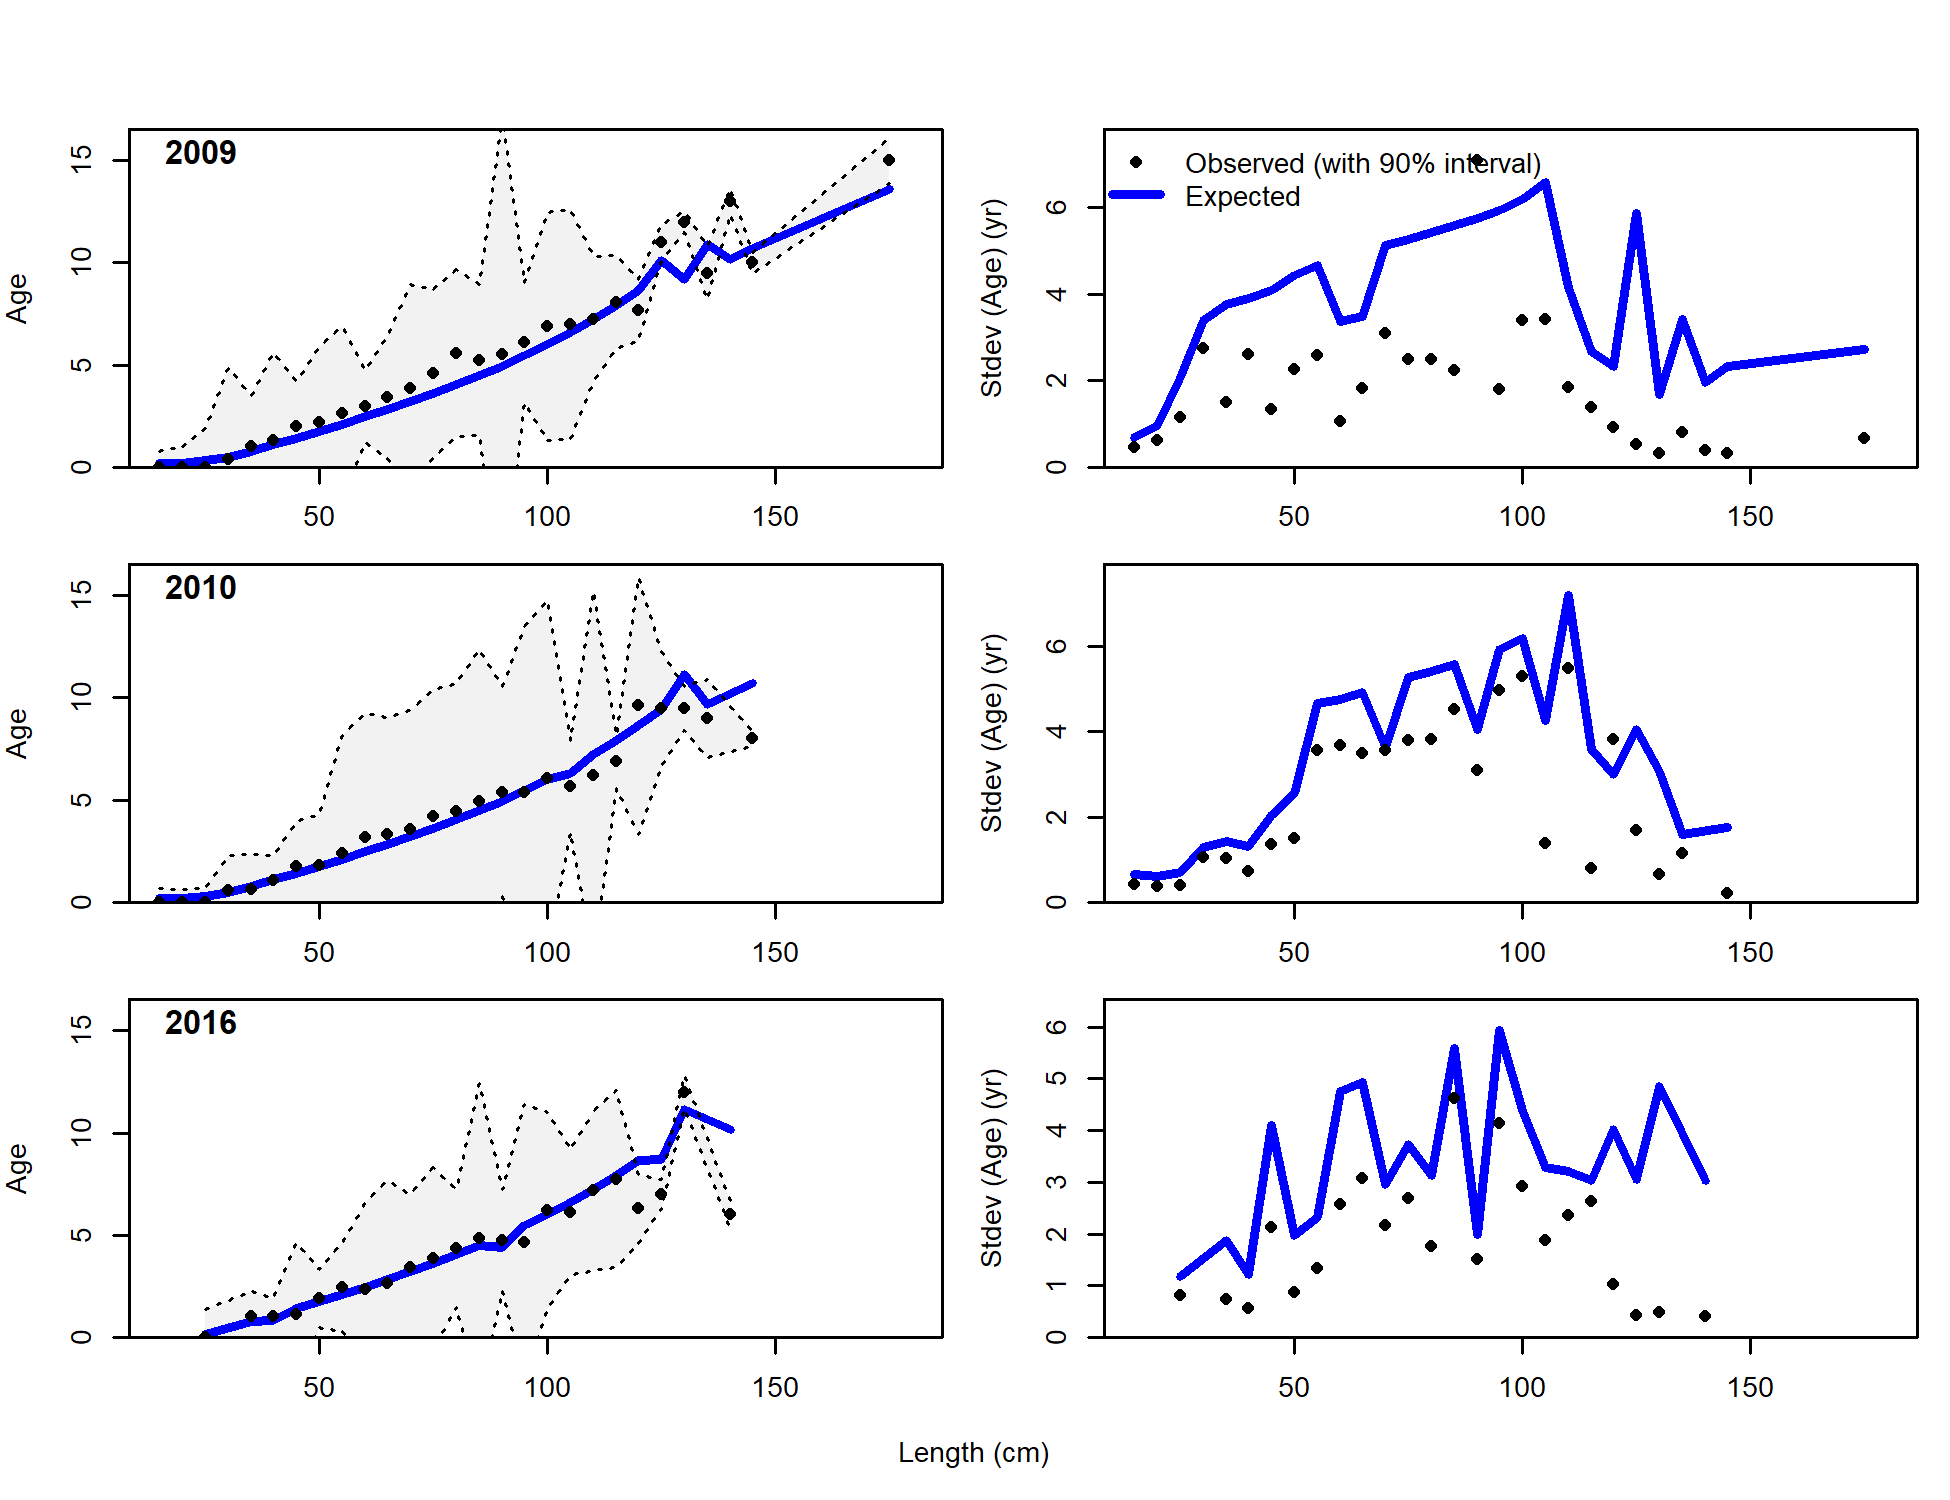
\includegraphics{./r4ss/plots_mod1/comp_condAALfit_Andre_plotsflt5mkt0_page1.png}
\caption{Conditional AAL plot, whole catch, Triennial Survey (plot 1 of
2) These plots show mean age and std. dev. in conditional AAL. Left
plots are mean AAL by size\_class (obs. and pred.) with 90\% CIs based
on adding 1.64 SE of mean to the data. Right plots in each pair are SE
of mean AAL (obs. and pred.) with 90\% CIs based on the chi\_square
distribution.
\label{fig:mod1_8_comp_condAALfit_Andre_plotsflt5mkt0_page1}}
\end{figure}

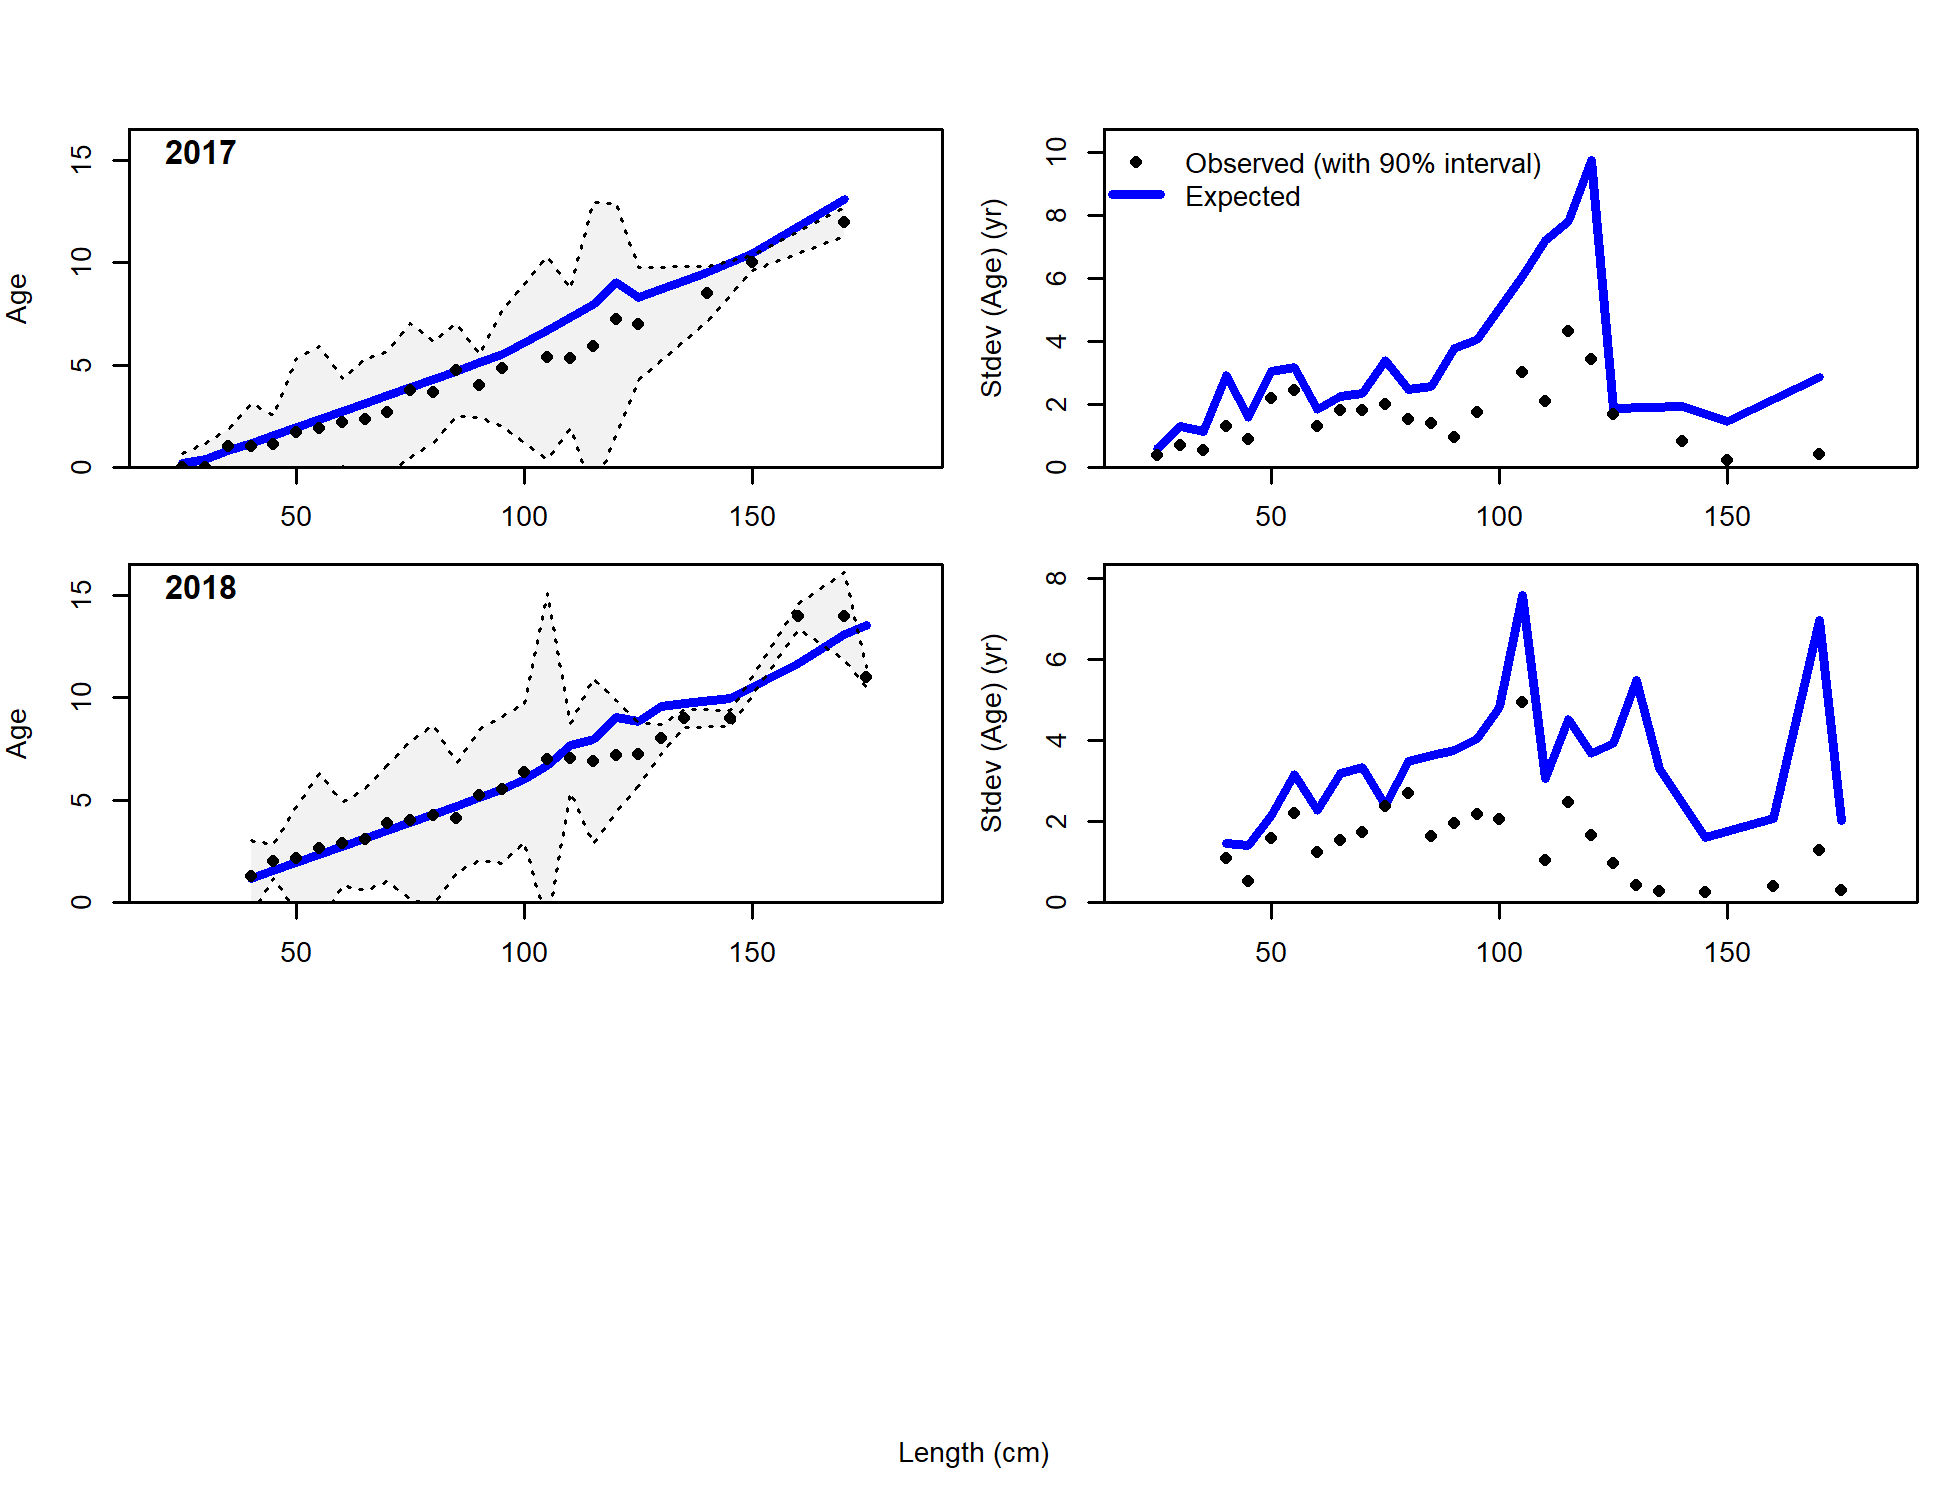
\includegraphics{./r4ss/plots_mod1/comp_condAALfit_Andre_plotsflt5mkt0_page2.png}

\begin{center} 

              Figure continued from previous page 

             \end{center}

\FloatBarrier

\FloatBarrier

\FloatBarrier

\FloatBarrier

\begin{figure}
\centering
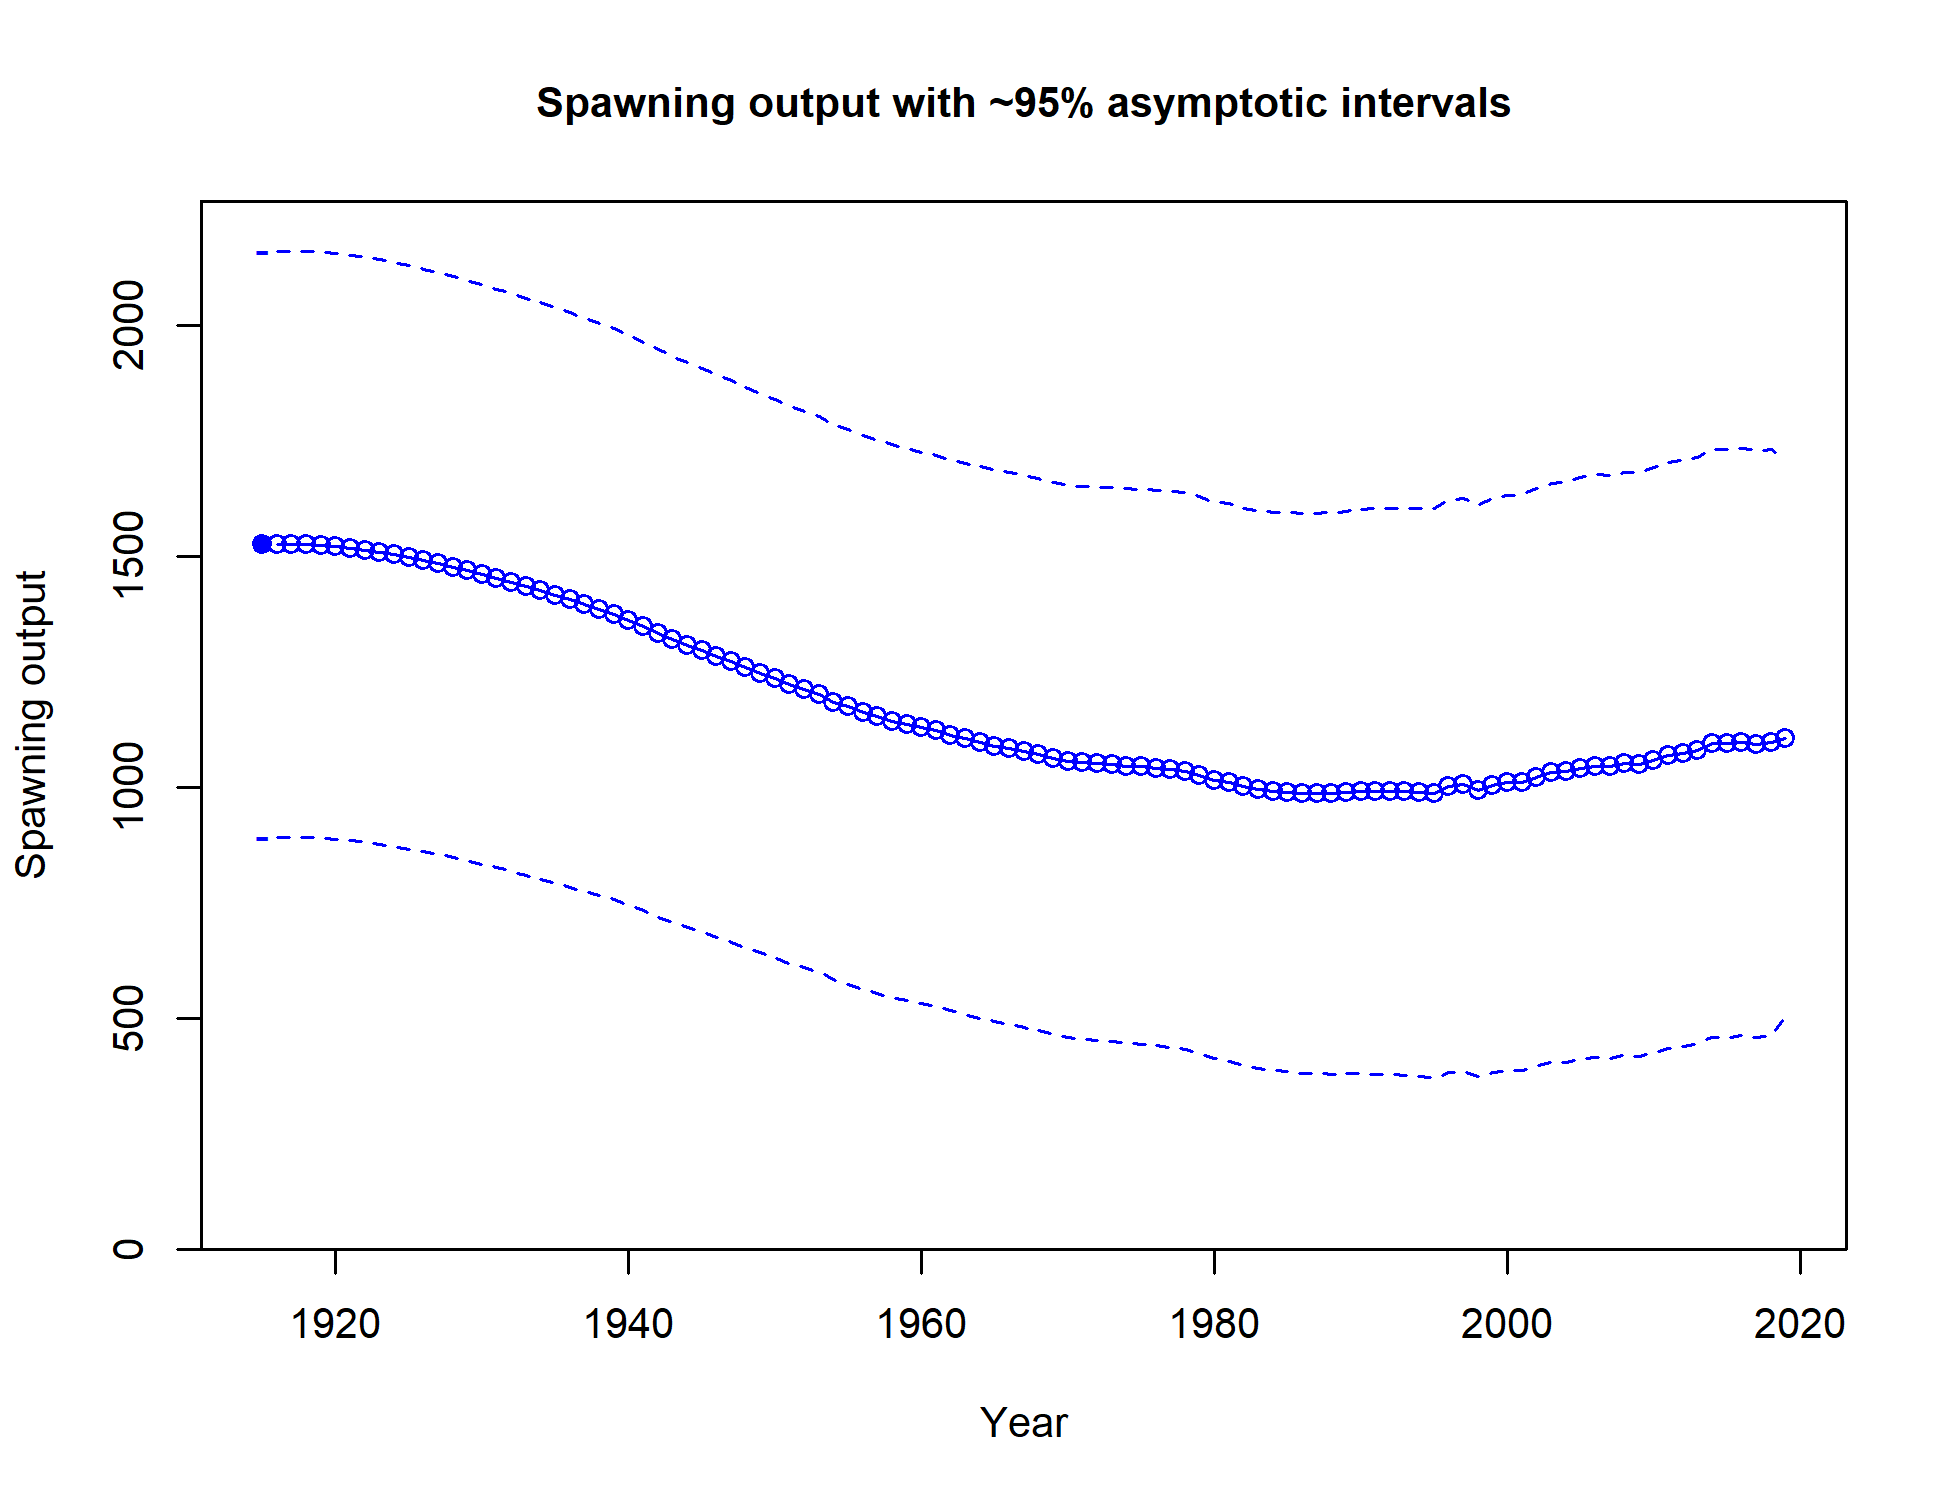
\includegraphics{r4ss/plots_mod1/ts7_Spawning_output_with_95_asymptotic_intervals_intervals.png}
\caption{Estimated spawning biomass (mt) with approximate 95\%
asymptotic intervals.
\label{fig:ts7_Spawning_biomass_(mt)_with_95_asymptotic_intervals_intervals}}
\end{figure}

\begin{figure}
\centering
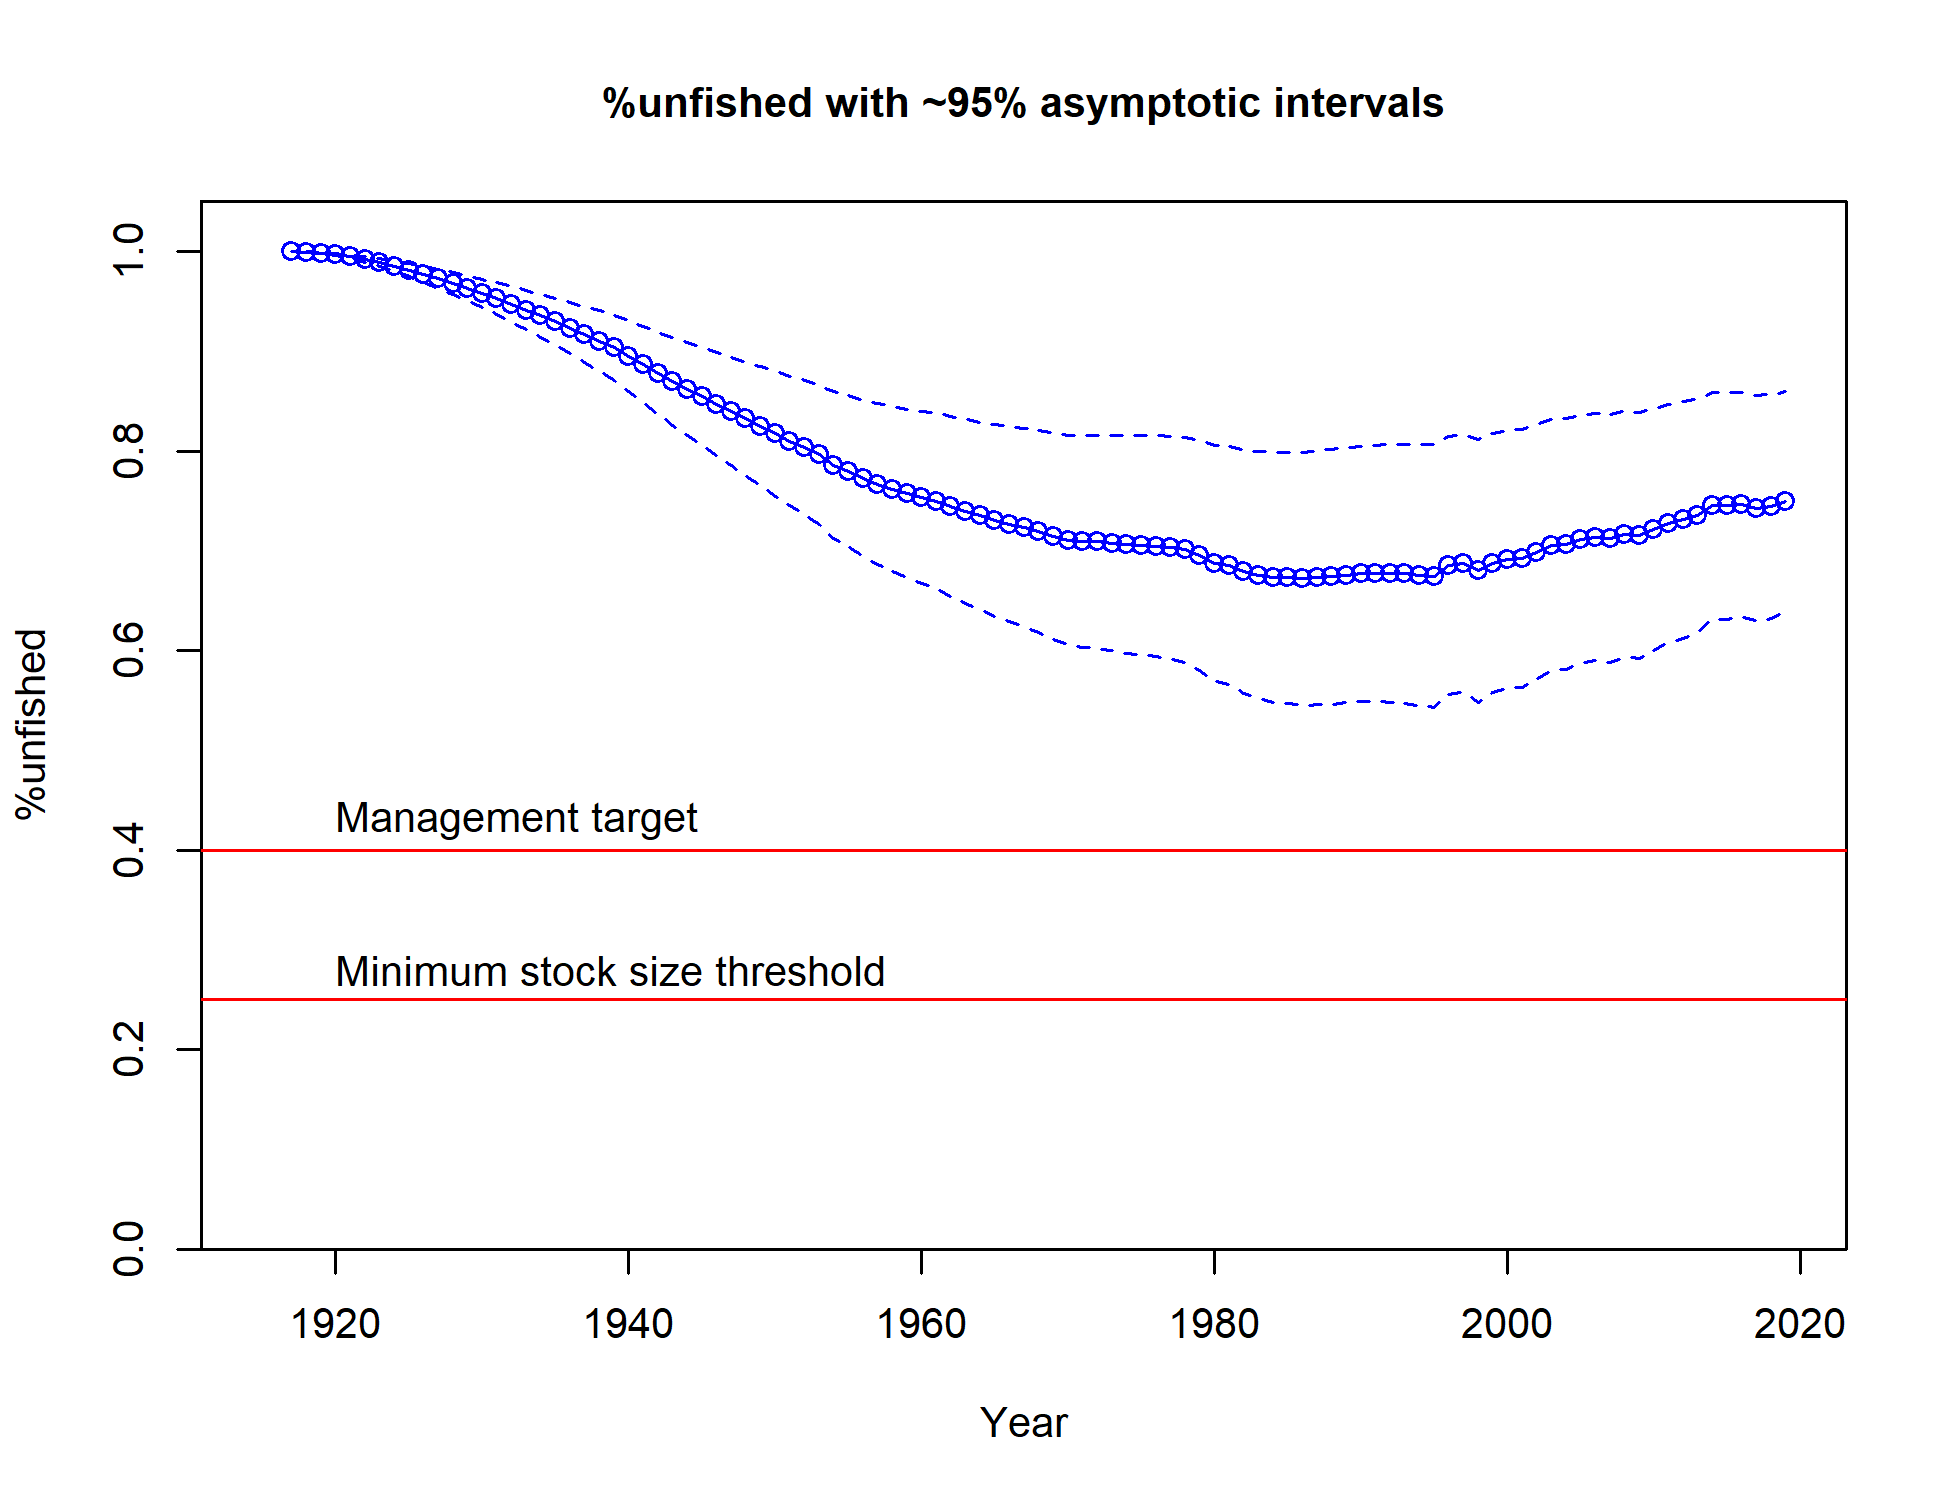
\includegraphics{r4ss/plots_mod1/ts9_Spawning_depletion_with_95_asymptotic_intervals_intervals.png}
\caption{Estimated spawning depletion with approximate 95\% asymptotic
intervals.
\label{fig:ts9_Spawning_depletion_with_95_asymptotic_intervals_intervals}}
\end{figure}

\begin{figure}
\centering
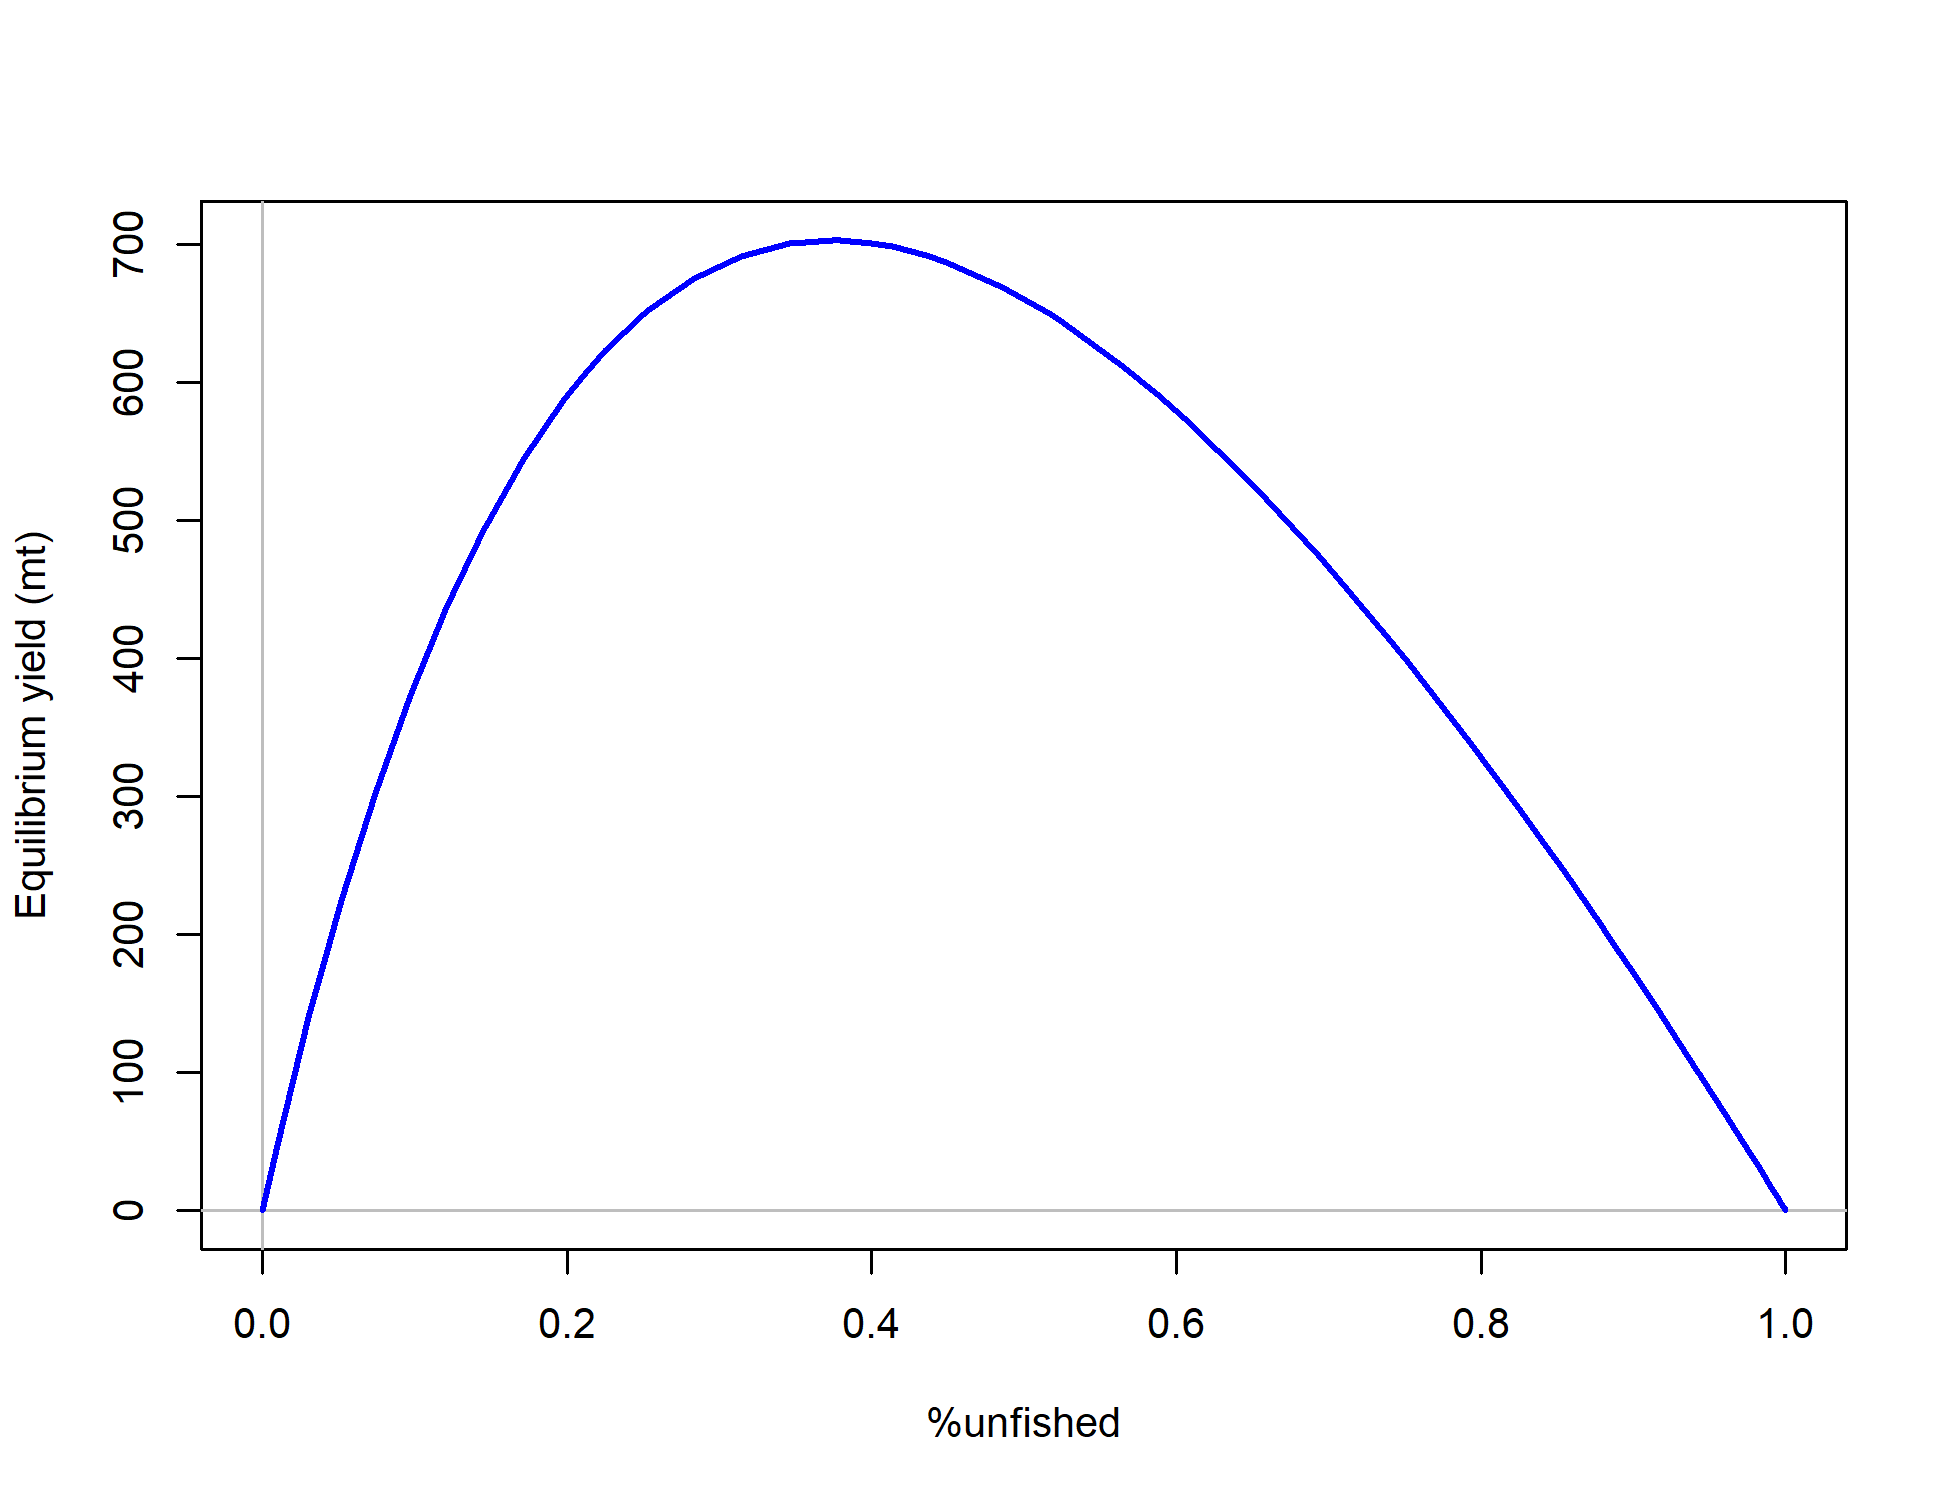
\includegraphics{r4ss/plots_mod1/yield1_yield_curve.png}
\caption{Equilibrium yield curve for the base case model. Values are
based on the 2018 fishery selectivity and with steepness fixed at 0.718.
\label{fig:yield1_yield_curve}}
\end{figure}

\FloatBarrier

\newpage

\FloatBarrier
\newpage

\#Appendix A. Detailed fits to length composition data \{-\}
\renewcommand{\thepage}{A-\arabic{page}}

\renewcommand{\thefigure}{A\arabic{figure}}
\setcounter{page}{1}

\begin{figure}
\centering
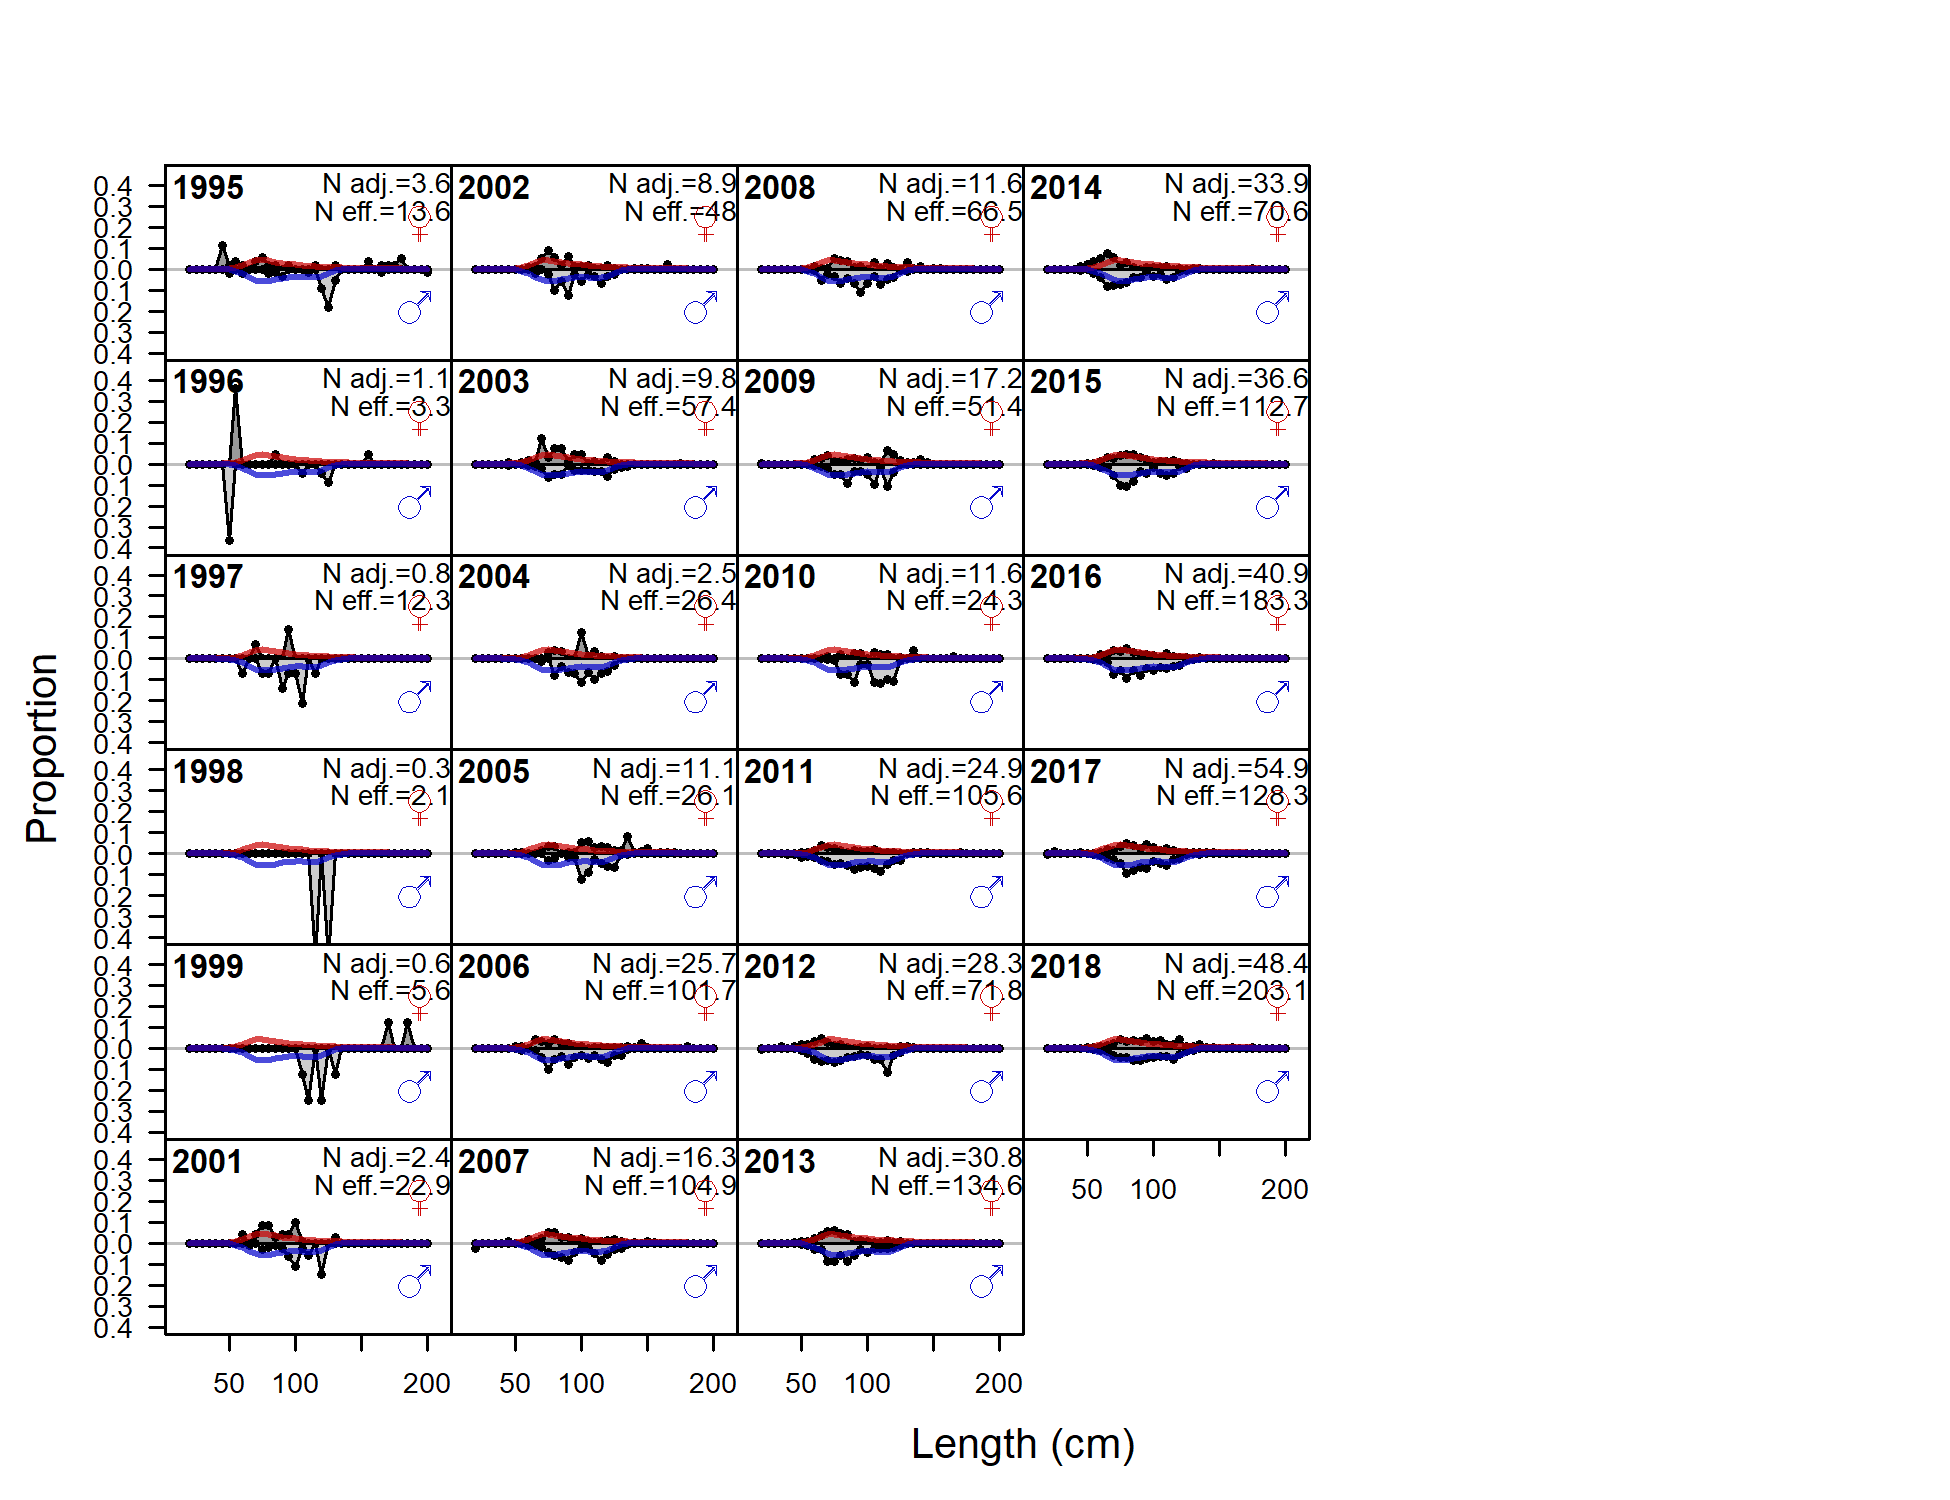
\includegraphics{./r4ss/plots_mod1/comp_lenfit_flt1mkt2.png}
\caption{Length comps, retained, Fishery. `N adj.' is the input sample
size after data\_weighting adjustment. N eff. is the calculated
effective sample size used in the McAllister\_Iannelli tuning method.
\label{fig:mod1_1_comp_lenfit_flt1mkt2}}
\end{figure}

\begin{figure}
\centering
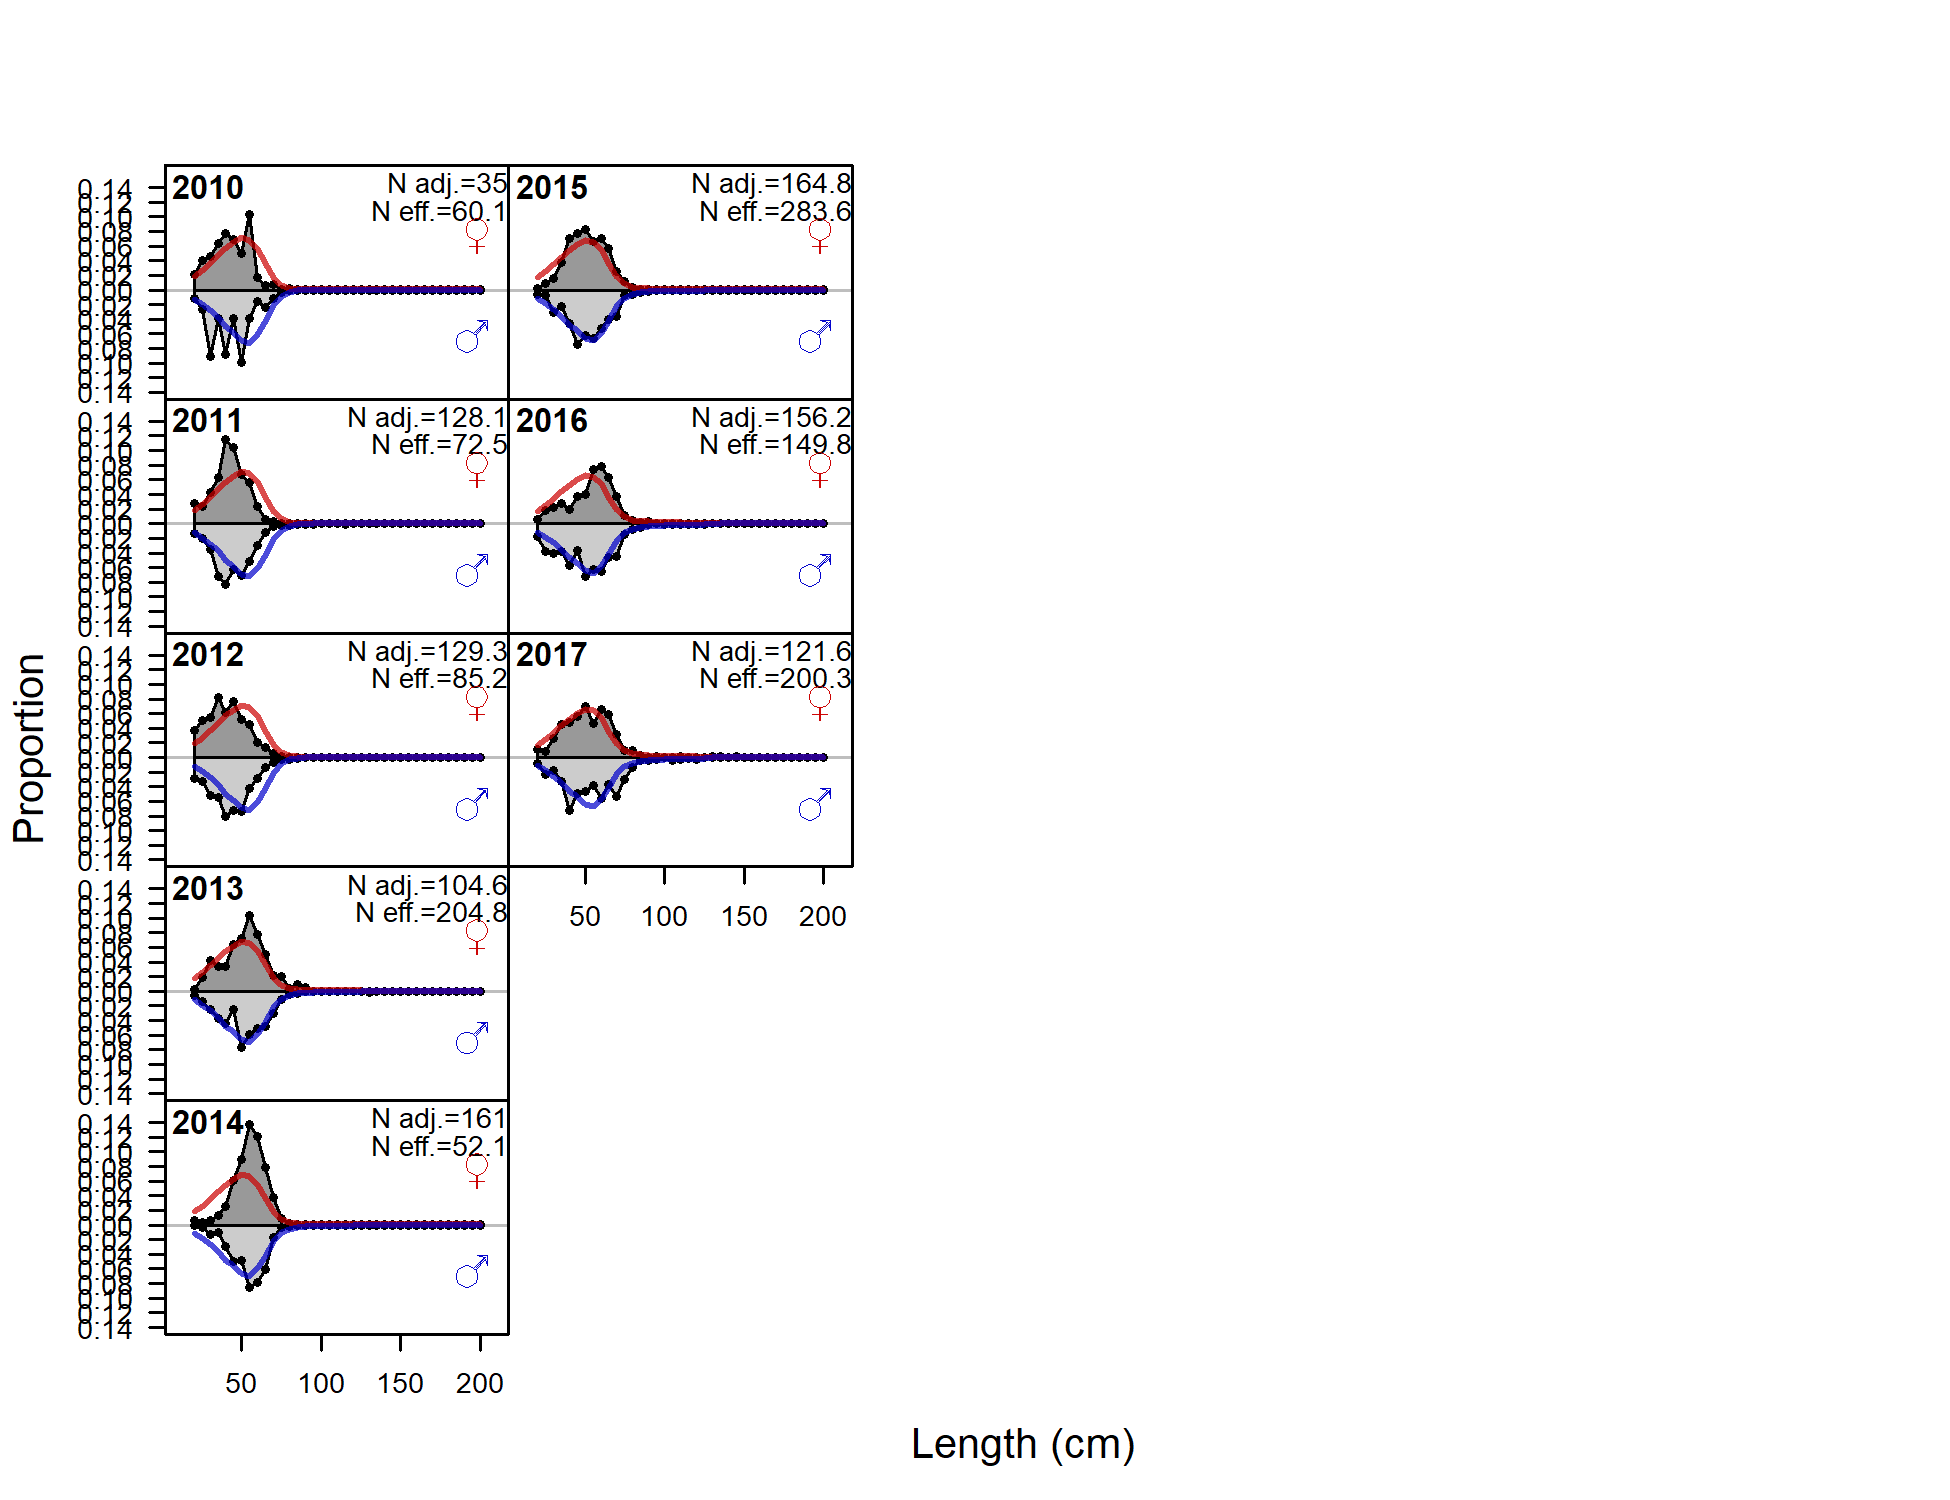
\includegraphics{./r4ss/plots_mod1/comp_lenfit_flt1mkt1.png}
\caption{Length comps, discard, Fishery. `N adj.' is the input sample
size after data\_weighting adjustment. N eff. is the calculated
effective sample size used in the McAllister\_Iannelli tuning method.
\label{fig:mod1_2_comp_lenfit_flt1mkt1}}
\end{figure}

\begin{figure}
\centering
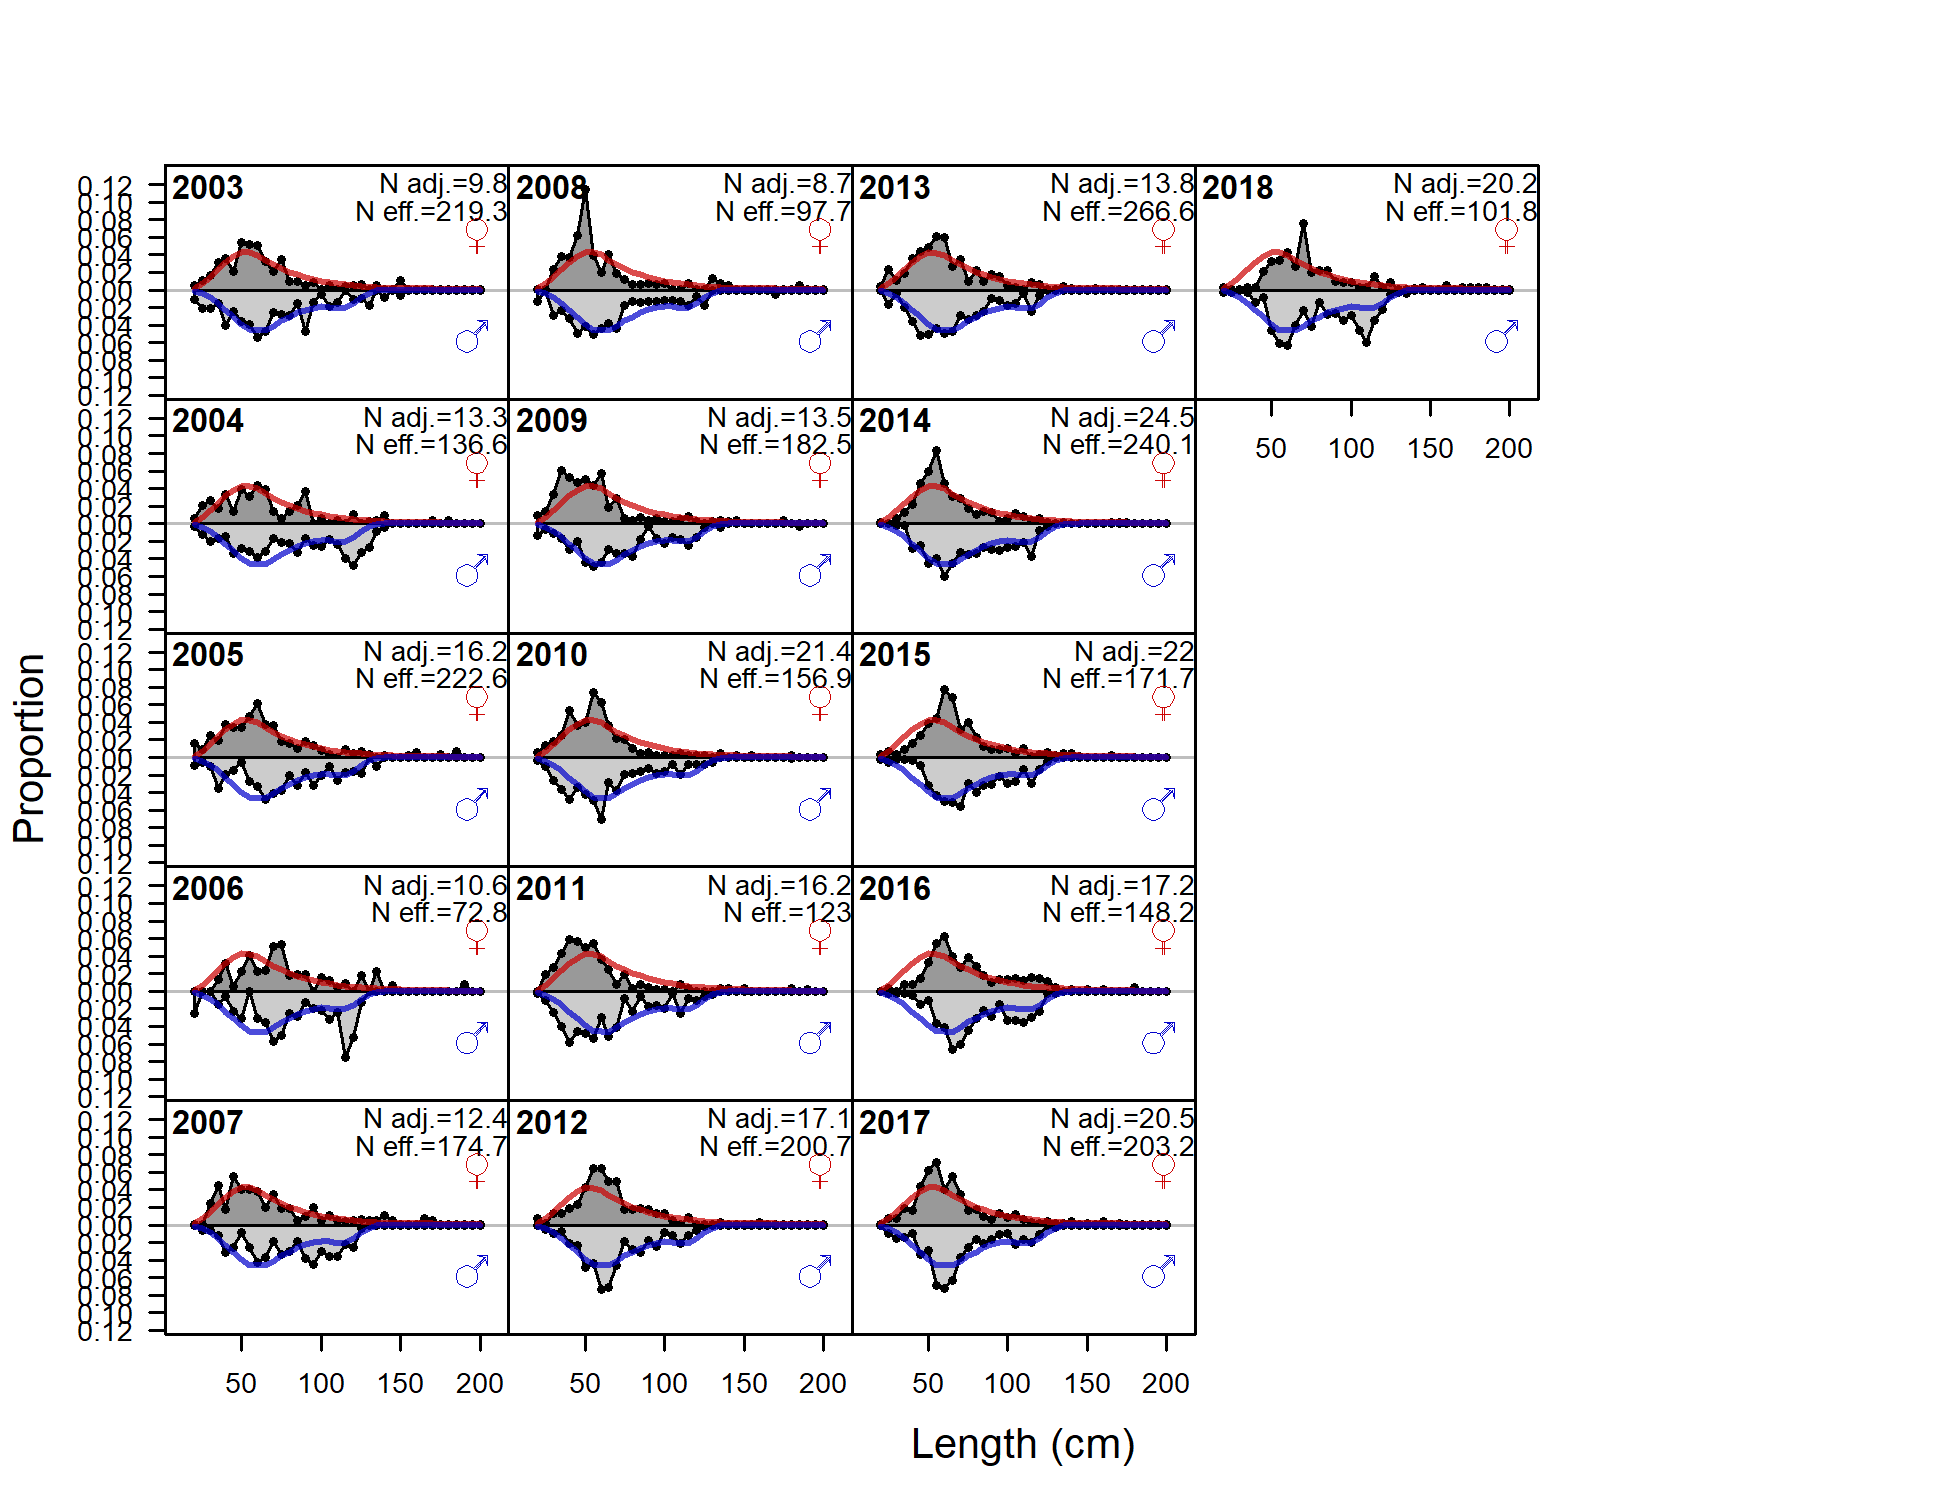
\includegraphics{./r4ss/plots_mod1/comp_lenfit_flt5mkt0.png}
\caption{Length comps, whole catch, Triennial Survey. `N adj.' is the
input sample size after data\_weighting adjustment. N eff. is the
calculated effective sample size used in the McAllister\_Iannelli tuning
method. \label{fig:mod1_3_comp_lenfit_flt5mkt0}}
\end{figure}

\begin{figure}
\centering
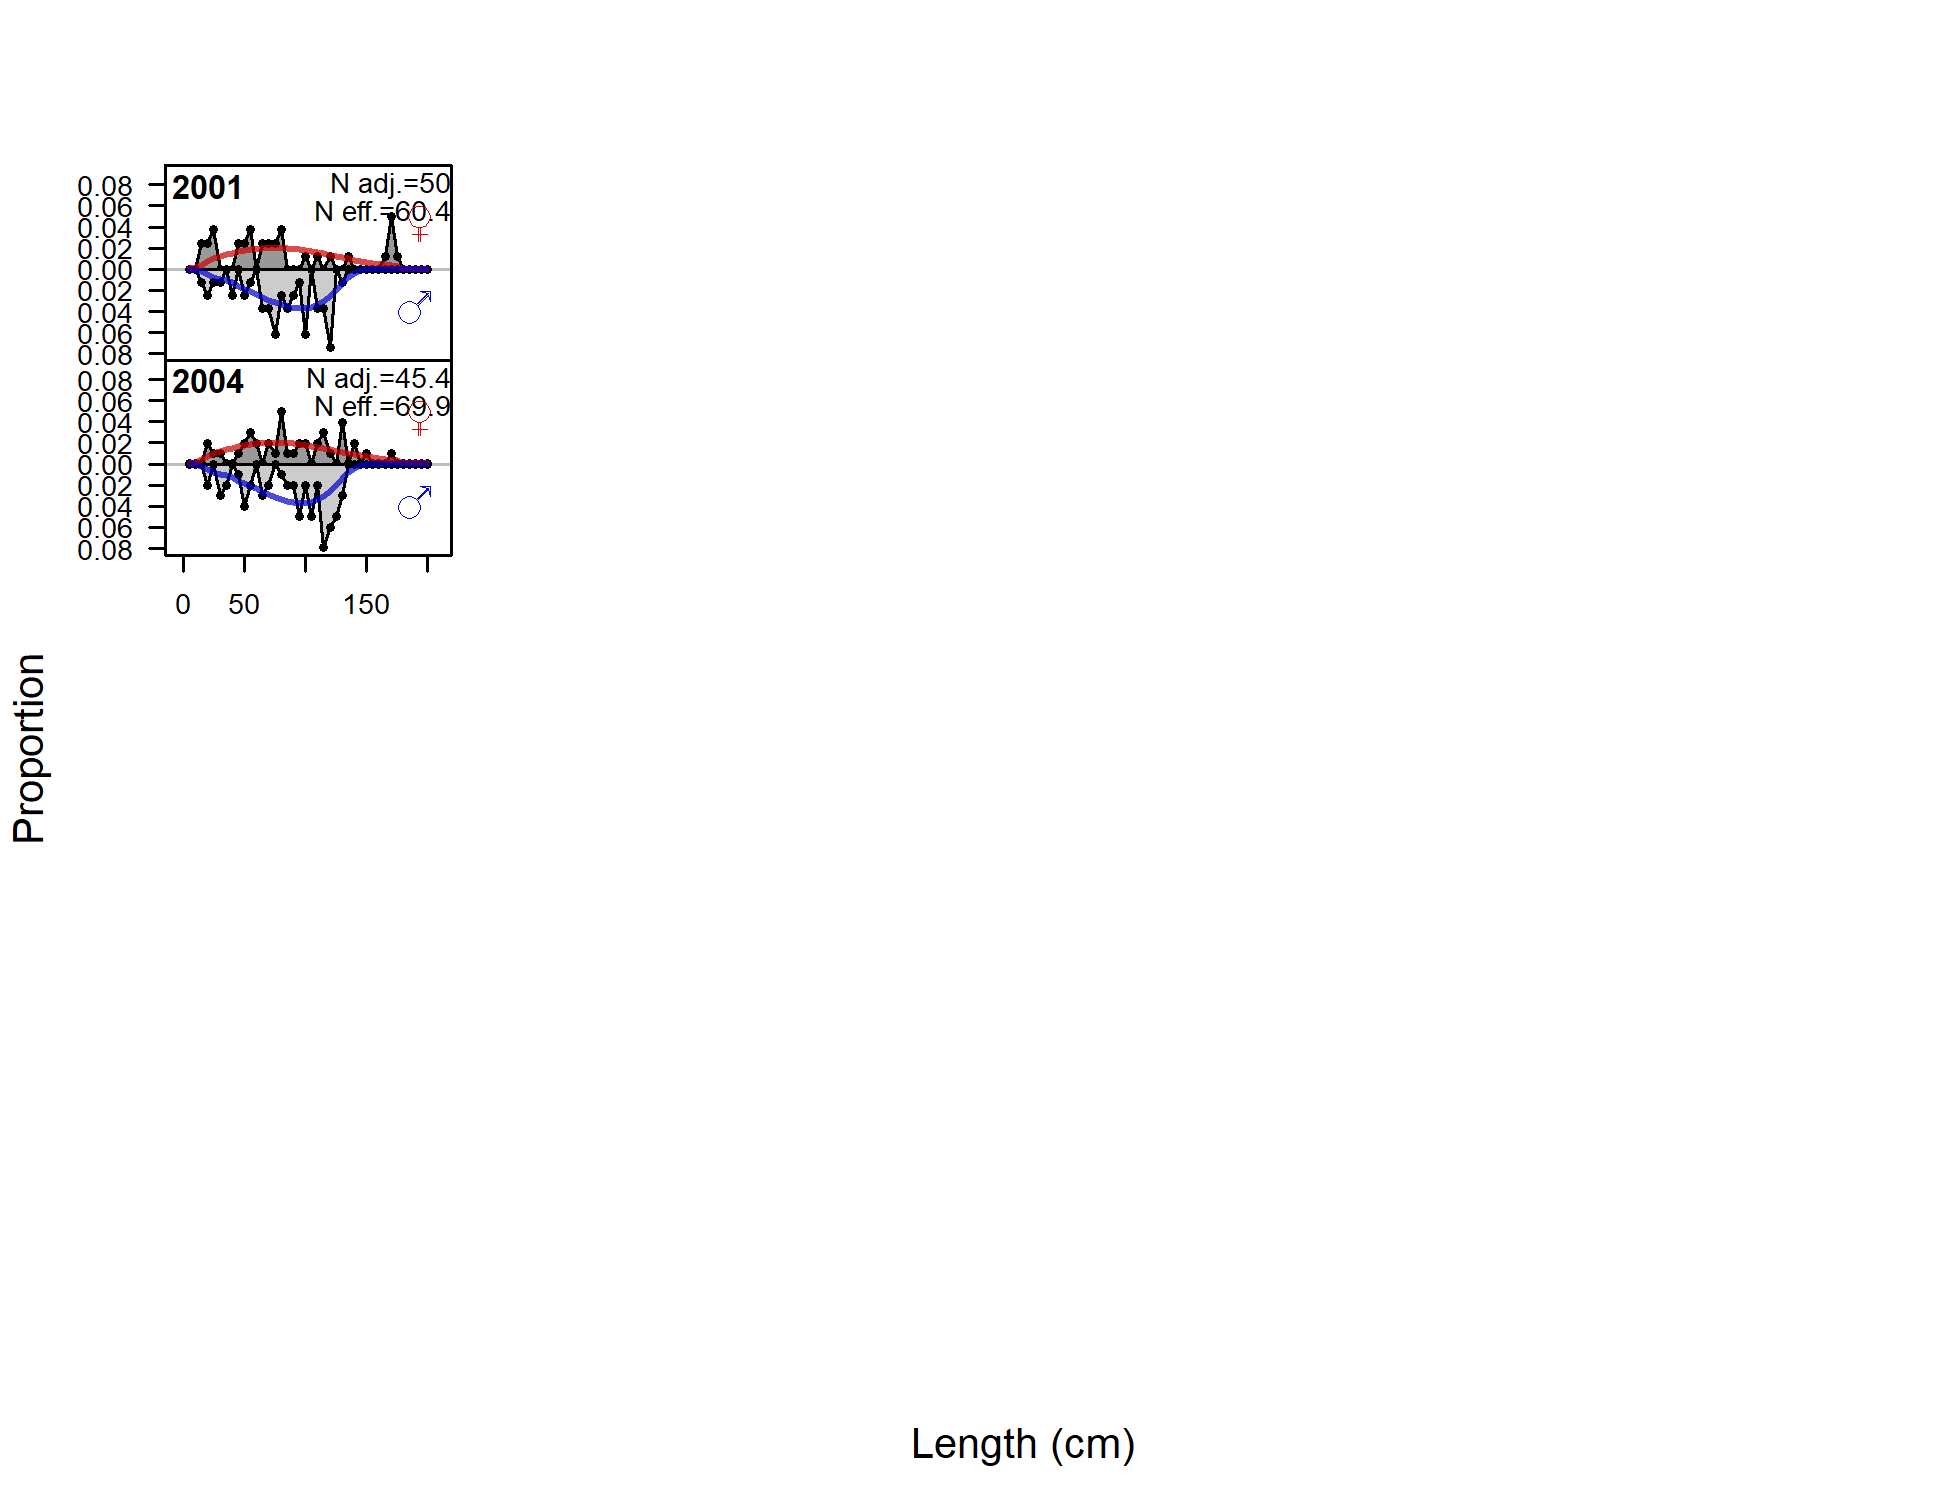
\includegraphics{./r4ss/plots_mod1/comp_lenfit_flt6mkt0.png}
\caption{Length comps, whole catch, WCGBT Survey. `N adj.' is the input
sample size after data\_weighting adjustment. N eff. is the calculated
effective sample size used in the McAllister\_Iannelli tuning method.
\label{fig:mod1_4_comp_lenfit_flt6mkt0}}
\end{figure}

\newpage

\color{black}

\hypertarget{references}{%
\section*{References}\label{references}}
\addcontentsline{toc}{section}{References}

\renewcommand{\thepage}{}

\hypertarget{refs}{}
\leavevmode\hypertarget{ref-AFSC2018}{}%
Alaska Fisheries Science Center. 2018. Assessment of the skate stock
complex in the Gulf of Alaska. Available from
\href{\%7B\%7Bhttps://www.afsc.noaa.gov/REFM/Docs/2018/GOA/GOAskate.pdf\%7D\%7D}{\{\{https://www.afsc.noaa.gov/REFM/Docs/2018/GOA/GOAskate.pdf\}\}}.

\leavevmode\hypertarget{ref-Batdorf1990}{}%
Batdorf, C. 1990. Northwest Native Harvest. Hancock House Publishers
Ltd.; Surrey, B.C., Canada.

\leavevmode\hypertarget{ref-Bizzarro2015}{}%
Bizzarro, J. 2015. Comparative resource utilization of eastern north
pacific skates (rajiformes: Rajidae) with applications for
ecosystem-based fisheries management. WA: University of Washington.

\leavevmode\hypertarget{ref-Bizzarro2019}{}%
Bizzarro, J. 2019. Manuscript in preparation.

\leavevmode\hypertarget{ref-Bizzarro2014}{}%
Bizzarro, JJ and Broms, KM and Logsdon, MG and Ebert, DA and Yoklavich,
MM and Kuhnz, LA and Summers, AP. 2014. Spatial segregation in eastern
north Pacific skate assemblages. PloS one \textbf{9}(10).

\leavevmode\hypertarget{ref-Bowers1909}{}%
Bowers, G. M. 1909. Report of The Commissioner For the Year Ending June
30, 1909. Part XXVIII. Washington Printing Office.

\leavevmode\hypertarget{ref-Bradburn2011}{}%
Bradburn, M.J. and Keller, A.A and Horness, B.H. 2011. The 2003 to 2008
US West Coast bottom trawl surveys of groundfish resources off
Washington, Oregon, and California: estimates of distribution,
abundance, length, and age composition. NOAA Technical Memorandum NMFS
NOAA-TM-NMFS-NWFSC-114: 323 pp.

\leavevmode\hypertarget{ref-TedCalavan}{}%
Calavan, T. 2019. Oregon Department of Fisheries; Wildlife; Personal
Communication, Newport, OR, USA.

\leavevmode\hypertarget{ref-Castro1996}{}%
Castro-Aguirre, J.L., and Pérez, H.E. 1996. Catálogo sistemático de las
rayas y especies afines de méxico: Chondrichthyes: Elasmobranchii:
Rajiformes: Batoideiomorpha. Unam.

\leavevmode\hypertarget{ref-Castro1993}{}%
Castro-Aguirre, J., Schmitter, J., Balart, E., and Torres-Orozco, R.
1993. On the geographical distribution of some bent ~'o nicos from the
west coast of baja california sur, m é xico, with ecological
considerations ~'o gicas y evoluutivas. \emph{In} Anales de la escuela
nacional de ciencias biol ~'o gicas, m é xico. pp. 75--102.

\leavevmode\hypertarget{ref-Chapman1944}{}%
Chapman, W.M. 1944. The Latent Fisheries of Washington and Alaska.
Washington State Department of Fisheries.

\leavevmode\hypertarget{ref-Chiquillo2014}{}%
Chiquillo, Kelcie L and Ebert, David A and Slager, Christina J and Crow,
Karen D. 2014. The secret of the mermaid's purse: Phylogenetic
affinities within the Rajidae and the evolution of a novel reproductive
strategy in skates. Molecular Phylogenetics and Evolution \textbf{75}:
245--251. Elsevier.

\leavevmode\hypertarget{ref-DeLacy1935}{}%
DeLacy, A.C., and Chapman, W.M. 1935. Notes on some elasmobranchs of
puget sound, with descriptions of their egg cases. Copeia
\textbf{1935}(2): 63--67. JSTOR.

\leavevmode\hypertarget{ref-Ebert2003}{}%
Ebert, D. 2003. Sharks, rays, and chimaeras of california. Univ of
California Press.

\leavevmode\hypertarget{ref-Ebert2007}{}%
Ebert, D.A., and Compagno, L.J. 2007. Biodiversity and systematics of
skates (chondrichthyes: Rajiformes: Rajoidei). \emph{In} Biology of
skates. Springer. pp. 5--18.

\leavevmode\hypertarget{ref-Ebert2008}{}%
Ebert, D.A., Smith, W.D., and Cailliet, G.M. 2008. Reproductive biology
of two commercially exploited skates, raja binoculata and r. Rhina, in
the western gulf of alaska. Fisheries Research \textbf{94}(1): 48--57.
Elsevier.

\leavevmode\hypertarget{ref-Eschmeyer1983}{}%
Eschmeyer, W.N., and Herald, E.S. 1983. A field guide to pacific coast
fishes: North america. Houghton Mifflin Harcourt.

\leavevmode\hypertarget{ref-Farrugia2016}{}%
Farrugia, T.J., Goldman, K.J., Tribuzio, C., and Seitz, A.C. 2016. First
use of satellite tags to examine movement and habitat use of big skates
beringraja binoculata in the gulf of alaska. Marine Ecology Progress
Series \textbf{556}: 209--221.

\leavevmode\hypertarget{ref-Ford1971}{}%
Ford, P. 1971. Differential growth rate in the tail of the pacific big
skate, (\emph{Raja binoculata}). Journal of the Fisheries Board of
Canada \textbf{28}(1): 95--98. NRC Research Press.

\leavevmode\hypertarget{ref-Gburski2007}{}%
Gburski, C.M. and Gaichas, S.K. and Kimura, D.K. 2007. Age and growth of
big skate (\emph{Raja binoculata}) and longnose skate (\emph{Raja
rhina}) in the Gulf of Alaska. \emph{In} Biology of Skates. Springer,
Dordrecht.

\leavevmode\hypertarget{ref-Gertseva2019}{}%
Gertseva, V. 2019. Manuscript in preparation.

\leavevmode\hypertarget{ref-Gunderson1980}{}%
Gunderson, Donald Raymond and Sample, Terrance M. 1980. Distribution and
abundance of rockfish off Washington, Oregon and California during 1977.
Northwest and Alaska Fisheries Center, National Marine Fisheries
Service. Available from
\href{\%7Bhttp://spo.nmfs.noaa.gov/mfr423-4/mfr423-42.pdf\%7D}{\{http://spo.nmfs.noaa.gov/mfr423-4/mfr423-42.pdf\}}.

\leavevmode\hypertarget{ref-Hamel2015}{}%
Hamel, Owen S. 2015. A method for calculating a meta-analytical prior
for the natural mortality rate using multiple life history correlates.
ICES Journal of Marine Science: Journal du Conseil \textbf{72}(1):
62--69. doi:
\href{https://doi.org/\%7B10.1093/icesjms/fsu131\%7D}{\{10.1093/icesjms/fsu131\}}.

\leavevmode\hypertarget{ref-Hitz1964}{}%
Hitz, C.R. 1964. Observations on egg cases of the big skate (raja
binoculata girard) found in oregon coastal waters. Journal of the
Fisheries Board of Canada \textbf{21}(4): 851--854. NRC Research Press.

\leavevmode\hypertarget{ref-Hoff2009}{}%
Hoff, GR. 2009. Skate Bathyraja spp. egg predation in the eastern Bering
Sea. J. Fish. Biol. \textbf{74}: 250--269.

\leavevmode\hypertarget{ref-Ishihara2012}{}%
Ishihara, H., Treloar, M., Bor, P., Senou, H., and Jeong, C. 2012. The
comparative morphology of skate egg capsules (Chondrichthyes:
Elasmobranchii: Rajiformes). Bulletin of the Kanagawa Prefectural Museum
(Natural Science) \textbf{41}: 9--25.

\leavevmode\hypertarget{ref-Keller2017}{}%
Keller, A.A. and Wallace, J.R. and Methot, R.D. 2017. The Northwest
Fisheries Science Center's West Coast Groundfish Bottom Trawl Survey:
History, Design, and Description. NOAA Technical Memorandum NMFS
NOAA-TM-NMFS-NWFSC-136: 38 pp.

\leavevmode\hypertarget{ref-KingandMcF2009}{}%
King, J., and McFarlane, G. 2009. Biological results of the strait of
georgia spiny dogfish (squalus acanthias) longline survey, october
10-22, 2008. Fisheries; Oceans Canada, Science Branch, Pacific Region.

\leavevmode\hypertarget{ref-King2015}{}%
King, J.R., Surry, A.M., Garcia, S., and P.J. Starr. 2015. Big skate
(Raja binoculata) and longnose skate (R. rhina) stock assessments for
British Columbia. Ottawa : Canadian Science Advisory Secretariat.

\leavevmode\hypertarget{ref-KingandMcF2010}{}%
King, JR and McFarlane, GA. 2010. Movement patterns and growth estimates
of big skate (\emph{Raja binoculata}) based on tag-recapture data. Fish.
Res. \textbf{101}: 50--59.

\leavevmode\hypertarget{ref-GregLippert}{}%
Lippert, G. 2019. Washington Department of Fisheries; Wildlife; Personal
Communication, Olympia, Washington, USA.

\leavevmode\hypertarget{ref-Love2011}{}%
Love, Milton S. 2011. Certainly more than you want to know about the
fishes of the Pacific Coast: a postmodern experience. Really Big Press.

\leavevmode\hypertarget{ref-Love1987}{}%
Love, Milton S and Axell, Brita and Morris, Pamela and Collins, Robson
and Brooks, Andrew. 1987. Life history and fishery of the California
scorpionfish,\\
emphScorpaena guttata, within the Southern California Bight. Fishery
Bulletin \textbf{85}: 99--116.

\leavevmode\hypertarget{ref-McEachran1990}{}%
McEachran, J., and Miyake, T. 1990. 1990. Zoogeography and bathymetry of
skates (chondrichthyes, rajidae). Elasmobranchs as living resources.
Advances in biology, Ecology, Systematics and the status of the
fisheries: 305--326.

\leavevmode\hypertarget{ref-McFandKing2006}{}%
McFarlane GA and King JR. 2006. Age and growth of big skate (\emph{Raja
binoculata}) and longnose skate (\emph{Raja rhina}) in British Columbia
waters. Fisheries Research \textbf{May 1 (2-3)}: 169--78.

\leavevmode\hypertarget{ref-Mecklenburg2002}{}%
Mecklenburg, CW and Mecklenburg, TA and Thorsteinson, LK. 2002. Fishes
of Alaska. American Fisheries Society, Bethesda, Maryland.

\leavevmode\hypertarget{ref-Miller1980}{}%
Miller, B.S., Cross, J.N., Steinfort, S.N., Fresh, K.L., and Simenstad,
C.A. 1980. Nearshore fish and macroinvertebrate assemblages along the
strait of juan de fuca including food habits of the common nearshore
fish.

\leavevmode\hypertarget{ref-Stevenson2008}{}%
Stevenson, DE and Orr, JW and Hoff, GR and McEachran, JD. 2008. Emerging
patterns of species richness, diversity, population density, and
distribution in the skates (Rajidae) of Alaska. Fish Bull \textbf{106}:
24--39.

\leavevmode\hypertarget{ref-Thorson2017a}{}%
Thorson, James T. and Barnett, Lewis A. K. 2017. Comparing estimates of
abundance trends and distribution shifts using single- and multispecies
models of fishes and biogenic habitat. ICES Journal of Marine Science:
Journal du Conseil: fsw193. doi:
\href{https://doi.org/\%7B10.1093/icesjms/fsw193\%7D}{\{10.1093/icesjms/fsw193\}}.

\leavevmode\hypertarget{ref-Thorson2015}{}%
Thorson, J. T. and Shelton, A. O. and Ward, E. J. and Skaug, H. J. 2015.
Geostatistical delta-generalized linear mixed models improve precision
for estimated abundance indices for West Coast groundfishes. ICES
Journal of Marine Science \textbf{72}(5): 1297--1310. doi:
\href{https://doi.org/\%7B10.1093/icesjms/fsu243\%7D}{\{10.1093/icesjms/fsu243\}}.

\leavevmode\hypertarget{ref-VonB}{}%
von Bertalanffy, L. 1938. A quantitative theory of organic growth. Human
Biology \textbf{10}: 181--213.

\leavevmode\hypertarget{ref-ZeinerWolf1993}{}%
Zeiner, S.J. and P. Wolf. 1993. Growth characteristics and estimates of
age at maturity of two species of skates (\emph{Raja binoculata}) and
(\emph{Raja rhina}) from Monterey Bay, California.

\end{document}
